% Generated by Sphinx.
\def\sphinxdocclass{report}
\documentclass[letterpaper,10pt,english]{sphinxmanual}
\usepackage[utf8]{inputenc}
\DeclareUnicodeCharacter{00A0}{\nobreakspace}
\usepackage{cmap}
\usepackage[T1]{fontenc}
\usepackage{babel}
\usepackage{times}
\usepackage[Bjarne]{fncychap}
\usepackage{longtable}
\usepackage{sphinx}
\usepackage{multirow}

\addto\captionsenglish{\renewcommand{\figurename}{Fig. }}
\addto\captionsenglish{\renewcommand{\tablename}{Table }}
\floatname{literal-block}{Listing }



\title{pydfnworks Documentation}
\date{March 09, 2017}
\release{2.0}
\author{Computational Earth Science (EES-16), LANL, LA-CC-17-027}
\newcommand{\sphinxlogo}{
\includegraphics{dfnworks_logo.png}\par}
\renewcommand{\releasename}{Release}
\makeindex

\makeatletter
\def\PYG@reset{\let\PYG@it=\relax \let\PYG@bf=\relax%
    \let\PYG@ul=\relax \let\PYG@tc=\relax%
    \let\PYG@bc=\relax \let\PYG@ff=\relax}
\def\PYG@tok#1{\csname PYG@tok@#1\endcsname}
\def\PYG@toks#1+{\ifx\relax#1\empty\else%
    \PYG@tok{#1}\expandafter\PYG@toks\fi}
\def\PYG@do#1{\PYG@bc{\PYG@tc{\PYG@ul{%
    \PYG@it{\PYG@bf{\PYG@ff{#1}}}}}}}
\def\PYG#1#2{\PYG@reset\PYG@toks#1+\relax+\PYG@do{#2}}

\expandafter\def\csname PYG@tok@gd\endcsname{\def\PYG@tc##1{\textcolor[rgb]{0.63,0.00,0.00}{##1}}}
\expandafter\def\csname PYG@tok@gu\endcsname{\let\PYG@bf=\textbf\def\PYG@tc##1{\textcolor[rgb]{0.50,0.00,0.50}{##1}}}
\expandafter\def\csname PYG@tok@gt\endcsname{\def\PYG@tc##1{\textcolor[rgb]{0.00,0.27,0.87}{##1}}}
\expandafter\def\csname PYG@tok@gs\endcsname{\let\PYG@bf=\textbf}
\expandafter\def\csname PYG@tok@gr\endcsname{\def\PYG@tc##1{\textcolor[rgb]{1.00,0.00,0.00}{##1}}}
\expandafter\def\csname PYG@tok@cm\endcsname{\let\PYG@it=\textit\def\PYG@tc##1{\textcolor[rgb]{0.25,0.50,0.56}{##1}}}
\expandafter\def\csname PYG@tok@vg\endcsname{\def\PYG@tc##1{\textcolor[rgb]{0.73,0.38,0.84}{##1}}}
\expandafter\def\csname PYG@tok@m\endcsname{\def\PYG@tc##1{\textcolor[rgb]{0.13,0.50,0.31}{##1}}}
\expandafter\def\csname PYG@tok@mh\endcsname{\def\PYG@tc##1{\textcolor[rgb]{0.13,0.50,0.31}{##1}}}
\expandafter\def\csname PYG@tok@cs\endcsname{\def\PYG@tc##1{\textcolor[rgb]{0.25,0.50,0.56}{##1}}\def\PYG@bc##1{\setlength{\fboxsep}{0pt}\colorbox[rgb]{1.00,0.94,0.94}{\strut ##1}}}
\expandafter\def\csname PYG@tok@ge\endcsname{\let\PYG@it=\textit}
\expandafter\def\csname PYG@tok@vc\endcsname{\def\PYG@tc##1{\textcolor[rgb]{0.73,0.38,0.84}{##1}}}
\expandafter\def\csname PYG@tok@il\endcsname{\def\PYG@tc##1{\textcolor[rgb]{0.13,0.50,0.31}{##1}}}
\expandafter\def\csname PYG@tok@go\endcsname{\def\PYG@tc##1{\textcolor[rgb]{0.20,0.20,0.20}{##1}}}
\expandafter\def\csname PYG@tok@cp\endcsname{\def\PYG@tc##1{\textcolor[rgb]{0.00,0.44,0.13}{##1}}}
\expandafter\def\csname PYG@tok@gi\endcsname{\def\PYG@tc##1{\textcolor[rgb]{0.00,0.63,0.00}{##1}}}
\expandafter\def\csname PYG@tok@gh\endcsname{\let\PYG@bf=\textbf\def\PYG@tc##1{\textcolor[rgb]{0.00,0.00,0.50}{##1}}}
\expandafter\def\csname PYG@tok@ni\endcsname{\let\PYG@bf=\textbf\def\PYG@tc##1{\textcolor[rgb]{0.84,0.33,0.22}{##1}}}
\expandafter\def\csname PYG@tok@nl\endcsname{\let\PYG@bf=\textbf\def\PYG@tc##1{\textcolor[rgb]{0.00,0.13,0.44}{##1}}}
\expandafter\def\csname PYG@tok@nn\endcsname{\let\PYG@bf=\textbf\def\PYG@tc##1{\textcolor[rgb]{0.05,0.52,0.71}{##1}}}
\expandafter\def\csname PYG@tok@no\endcsname{\def\PYG@tc##1{\textcolor[rgb]{0.38,0.68,0.84}{##1}}}
\expandafter\def\csname PYG@tok@na\endcsname{\def\PYG@tc##1{\textcolor[rgb]{0.25,0.44,0.63}{##1}}}
\expandafter\def\csname PYG@tok@nb\endcsname{\def\PYG@tc##1{\textcolor[rgb]{0.00,0.44,0.13}{##1}}}
\expandafter\def\csname PYG@tok@nc\endcsname{\let\PYG@bf=\textbf\def\PYG@tc##1{\textcolor[rgb]{0.05,0.52,0.71}{##1}}}
\expandafter\def\csname PYG@tok@nd\endcsname{\let\PYG@bf=\textbf\def\PYG@tc##1{\textcolor[rgb]{0.33,0.33,0.33}{##1}}}
\expandafter\def\csname PYG@tok@ne\endcsname{\def\PYG@tc##1{\textcolor[rgb]{0.00,0.44,0.13}{##1}}}
\expandafter\def\csname PYG@tok@nf\endcsname{\def\PYG@tc##1{\textcolor[rgb]{0.02,0.16,0.49}{##1}}}
\expandafter\def\csname PYG@tok@si\endcsname{\let\PYG@it=\textit\def\PYG@tc##1{\textcolor[rgb]{0.44,0.63,0.82}{##1}}}
\expandafter\def\csname PYG@tok@s2\endcsname{\def\PYG@tc##1{\textcolor[rgb]{0.25,0.44,0.63}{##1}}}
\expandafter\def\csname PYG@tok@vi\endcsname{\def\PYG@tc##1{\textcolor[rgb]{0.73,0.38,0.84}{##1}}}
\expandafter\def\csname PYG@tok@nt\endcsname{\let\PYG@bf=\textbf\def\PYG@tc##1{\textcolor[rgb]{0.02,0.16,0.45}{##1}}}
\expandafter\def\csname PYG@tok@nv\endcsname{\def\PYG@tc##1{\textcolor[rgb]{0.73,0.38,0.84}{##1}}}
\expandafter\def\csname PYG@tok@s1\endcsname{\def\PYG@tc##1{\textcolor[rgb]{0.25,0.44,0.63}{##1}}}
\expandafter\def\csname PYG@tok@gp\endcsname{\let\PYG@bf=\textbf\def\PYG@tc##1{\textcolor[rgb]{0.78,0.36,0.04}{##1}}}
\expandafter\def\csname PYG@tok@sh\endcsname{\def\PYG@tc##1{\textcolor[rgb]{0.25,0.44,0.63}{##1}}}
\expandafter\def\csname PYG@tok@ow\endcsname{\let\PYG@bf=\textbf\def\PYG@tc##1{\textcolor[rgb]{0.00,0.44,0.13}{##1}}}
\expandafter\def\csname PYG@tok@sx\endcsname{\def\PYG@tc##1{\textcolor[rgb]{0.78,0.36,0.04}{##1}}}
\expandafter\def\csname PYG@tok@bp\endcsname{\def\PYG@tc##1{\textcolor[rgb]{0.00,0.44,0.13}{##1}}}
\expandafter\def\csname PYG@tok@c1\endcsname{\let\PYG@it=\textit\def\PYG@tc##1{\textcolor[rgb]{0.25,0.50,0.56}{##1}}}
\expandafter\def\csname PYG@tok@kc\endcsname{\let\PYG@bf=\textbf\def\PYG@tc##1{\textcolor[rgb]{0.00,0.44,0.13}{##1}}}
\expandafter\def\csname PYG@tok@c\endcsname{\let\PYG@it=\textit\def\PYG@tc##1{\textcolor[rgb]{0.25,0.50,0.56}{##1}}}
\expandafter\def\csname PYG@tok@mf\endcsname{\def\PYG@tc##1{\textcolor[rgb]{0.13,0.50,0.31}{##1}}}
\expandafter\def\csname PYG@tok@err\endcsname{\def\PYG@bc##1{\setlength{\fboxsep}{0pt}\fcolorbox[rgb]{1.00,0.00,0.00}{1,1,1}{\strut ##1}}}
\expandafter\def\csname PYG@tok@mb\endcsname{\def\PYG@tc##1{\textcolor[rgb]{0.13,0.50,0.31}{##1}}}
\expandafter\def\csname PYG@tok@ss\endcsname{\def\PYG@tc##1{\textcolor[rgb]{0.32,0.47,0.09}{##1}}}
\expandafter\def\csname PYG@tok@sr\endcsname{\def\PYG@tc##1{\textcolor[rgb]{0.14,0.33,0.53}{##1}}}
\expandafter\def\csname PYG@tok@mo\endcsname{\def\PYG@tc##1{\textcolor[rgb]{0.13,0.50,0.31}{##1}}}
\expandafter\def\csname PYG@tok@kd\endcsname{\let\PYG@bf=\textbf\def\PYG@tc##1{\textcolor[rgb]{0.00,0.44,0.13}{##1}}}
\expandafter\def\csname PYG@tok@mi\endcsname{\def\PYG@tc##1{\textcolor[rgb]{0.13,0.50,0.31}{##1}}}
\expandafter\def\csname PYG@tok@kn\endcsname{\let\PYG@bf=\textbf\def\PYG@tc##1{\textcolor[rgb]{0.00,0.44,0.13}{##1}}}
\expandafter\def\csname PYG@tok@o\endcsname{\def\PYG@tc##1{\textcolor[rgb]{0.40,0.40,0.40}{##1}}}
\expandafter\def\csname PYG@tok@kr\endcsname{\let\PYG@bf=\textbf\def\PYG@tc##1{\textcolor[rgb]{0.00,0.44,0.13}{##1}}}
\expandafter\def\csname PYG@tok@s\endcsname{\def\PYG@tc##1{\textcolor[rgb]{0.25,0.44,0.63}{##1}}}
\expandafter\def\csname PYG@tok@kp\endcsname{\def\PYG@tc##1{\textcolor[rgb]{0.00,0.44,0.13}{##1}}}
\expandafter\def\csname PYG@tok@w\endcsname{\def\PYG@tc##1{\textcolor[rgb]{0.73,0.73,0.73}{##1}}}
\expandafter\def\csname PYG@tok@kt\endcsname{\def\PYG@tc##1{\textcolor[rgb]{0.56,0.13,0.00}{##1}}}
\expandafter\def\csname PYG@tok@sc\endcsname{\def\PYG@tc##1{\textcolor[rgb]{0.25,0.44,0.63}{##1}}}
\expandafter\def\csname PYG@tok@sb\endcsname{\def\PYG@tc##1{\textcolor[rgb]{0.25,0.44,0.63}{##1}}}
\expandafter\def\csname PYG@tok@k\endcsname{\let\PYG@bf=\textbf\def\PYG@tc##1{\textcolor[rgb]{0.00,0.44,0.13}{##1}}}
\expandafter\def\csname PYG@tok@se\endcsname{\let\PYG@bf=\textbf\def\PYG@tc##1{\textcolor[rgb]{0.25,0.44,0.63}{##1}}}
\expandafter\def\csname PYG@tok@sd\endcsname{\let\PYG@it=\textit\def\PYG@tc##1{\textcolor[rgb]{0.25,0.44,0.63}{##1}}}

\def\PYGZbs{\char`\\}
\def\PYGZus{\char`\_}
\def\PYGZob{\char`\{}
\def\PYGZcb{\char`\}}
\def\PYGZca{\char`\^}
\def\PYGZam{\char`\&}
\def\PYGZlt{\char`\<}
\def\PYGZgt{\char`\>}
\def\PYGZsh{\char`\#}
\def\PYGZpc{\char`\%}
\def\PYGZdl{\char`\$}
\def\PYGZhy{\char`\-}
\def\PYGZsq{\char`\'}
\def\PYGZdq{\char`\"}
\def\PYGZti{\char`\~}
% for compatibility with earlier versions
\def\PYGZat{@}
\def\PYGZlb{[}
\def\PYGZrb{]}
\makeatother

\renewcommand\PYGZsq{\textquotesingle}

\begin{document}

\maketitle
\tableofcontents
\phantomsection\label{index::doc}


Contents:


\chapter{Introduction}
\label{intro:introduction}\label{intro:welcome-to-dfnworks-2-0-documentation}\label{intro::doc}
dfnWorks is a parallelized computational suite to generate three-dimensional discrete fracture networks (DFN) and simulate flow and transport. Developed at Los Alamos National Laboratory, it has been used to study flow and transport in fractured media at scales ranging from millimeters to kilometers. The networks are created and meshed using dfnGen, which combines FRAM (the feature rejection algorithm for meshing) methodology to stochastically generate three-dimensional DFNs with the LaGriT meshing toolbox to create a high-quality computational mesh representation. The representation produces a conforming Delaunay triangulation suitable for high performance computing finite volume solvers in an intrinsically parallel fashion. Flow through the network is simulated with dfnFlow, which utilizes the massively parallel subsurface flow and reactive transport finite volume code PFLOTRAN. A Lagrangian approach to simulating transport through the DFN is adopted within dfnTrans to determine pathlines and solute transport through the DFN. Applications of the dfnWorks suite include nuclear waste repository science, hydraulic fracturing and CO$_{\text{2}}$ sequestration.

To run a workflow using the dfnWorks suite, the pydfnworks package is highly recommended. pydfnworks calls various tools in the dfnWorks suite; its aim is to provide a seamless workflow for scientific applications of dfnWorks.


\section{Citing dfnWorks}
\label{intro:citing-dfnworks}
\href{http://www.sciencedirect.com/science/article/pii/S0098300415300261/}{Hyman, J. D., Karra, S., Makedonska, N., Gable, C. W., Painter, S. L., \& Viswanathan, H. S. (2015). dfnWorks: A discrete fracture network framework for modeling subsurface flow and transport. Computers \& Geosciences, 84, 10-19.}

\emph{BibTex:}

\begin{Verbatim}[commandchars=\\\{\}]
  @article\PYGZob{}hyman2015dfnworks,
    title=\PYGZob{}dfnWorks: A discrete fracture network framework
for modeling subsurface flow and transport\PYGZcb{},
    author=\PYGZob{}Hyman, Jeffrey D and Karra, Satish and Makedonska,
Nataliia and Gable, Carl W and Painter, Scott L
and Viswanathan, Hari S\PYGZcb{},
    journal=\PYGZob{}Computers \PYGZbs{}\PYGZam{} Geosciences\PYGZcb{},
    volume=\PYGZob{}84\PYGZcb{},
    pages=\PYGZob{}10\PYGZhy{}\PYGZhy{}19\PYGZcb{},
    year=\PYGZob{}2015\PYGZcb{},
    publisher=\PYGZob{}Elsevier\PYGZcb{}
  \PYGZcb{}
\end{Verbatim}


\section{What's new in v2.0?}
\label{intro:what-s-new-in-v2-0}\begin{itemize}
\item {} 
New dfnGen C++ code which is much faster than the Mathematica dfnGen. This code has successfully generated networks with 350,000+ fractures.

\item {} 
Increased functionality in the pydfnworks package for more streamlined workflow from dfnGen through visualization.

\end{itemize}


\section{Where can one get dfnWorks?}
\label{intro:where-can-one-get-dfnworks}
dfnWorks 2.0 can be downloaded from \href{https://github.com/dfnWorks/dfnWorks-Version2.0}{https://github.com/dfnWorks/dfnWorks-Version2.0}

v1.0 can be downloaded from \href{https://github.com/dfnWorks/dfnWorks-Version1.0}{https://github.com/dfnWorks/dfnWorks-Version1.0}


\section{Installation}
\label{intro:installation}
Tools that you will need to run the dfnWorks work flow are described in this section. VisIt and ParaView, which enable visualization of desired quantities on the DFNs, are optional, but at least one of them is highly recommended for visualization. CMake is also optional but allows faster IO processing using C++.


\subsection{Python}
\label{intro:python}
pydfnworks is supported on Python 2.7. The software authors recommend using the Anaconda 2.7 distribution of Python, available at \href{https://www.continuum.io/}{https://www.continuum.io/}.
pydfnworks requires the \code{numpy} and \code{h5py} modules to be installed.


\subsection{pydfnworks}
\label{intro:pydfnworks}
The source for pydfnworks can be found in the dfnWorks suite, in the folder pydfnworks.


\subsection{dfnGen}
\label{intro:dfngen}
dfnGen primarily involves two steps:
\begin{enumerate}
\item {} 
FRAM - Create DFN: Using the fractured site characterization networks are constructed using the feature rejection algorithm for meshing

\item {} 
LaGriT - Mesh DFN: The LaGriT meshing tool box is used to create a conforming Delaunay triangulation of the network.

\end{enumerate}


\subsubsection{FRAM}
\label{intro:fram}
FRAM (the feature rejection algorithm for meshing) is executed using the dfnGen C++ source code, contained in the dfnGen folder of the dfnWorks repository.


\subsubsection{LaGriT}
\label{intro:lagrit}
The {\hyperref[intro:lagrit]{\emph{LaGriT}}} (\href{http://lagrit.lanl.gov}{http://lagrit.lanl.gov}) meshing toolbox is used to create a high resolution computational mesh representation of the DFN in parallel. An algorithm for conforming Delaunay triangulation is implemented so that fracture intersections are coincident with triangle edges in the mesh and Voronoi control volumes are suitable for finite volume flow solvers such as FEHM and PFLOTRAN.


\subsection{dfnFlow}
\label{intro:dfnflow}
You will need one of either PFLOTRAN or FEHM to solve for flow using the mesh files from LaGriT.


\subsubsection{PFLOTRAN}
\label{intro:pflotran}
\href{https://www.pflotran.org/}{PFLOTRAN} (\href{http://www.pflotran.org}{http://www.pflotran.org}) is a massively parallel subsurface flow and reactive transport code. PFLOTRAN solves a system of partial differential equations for multiphase, multicomponent and multiscale reactive flow and transport in porous media. The code is designed to run on leadership-class supercomputers as well as workstations and laptops.


\subsubsection{FEHM}
\label{intro:fehm}\label{intro:id1}
{\hyperref[intro:fehm]{\emph{FEHM}}} (\href{http://fehm.lanl.gov}{http://fehm.lanl.gov}) is a subsurface multiphase flow code developed at Los Alamos National Laboratory.


\subsection{dfnTrans}
\label{intro:dfntrans}
dfnTrans is a method for resolving solute transport using control volume flow solutions obtained from dfnFlow on the unstructured mesh generated using dfnGen. We adopt a Lagrangian approach and represent a non-reactive conservative solute as a collection of indivisible passive tracer particles.


\subsection{CMake}
\label{intro:cmake}
CMake (\href{https://cmake.org/}{https://cmake.org/}) is an open-source, cross-platform family of tools designed to build, test and package software. It is needed to use C++ for processing files at a bottleneck IO step of dfnWorks. Using C+C++ for this file processing optional but can greatly increase the speed of dfnWorks for large fracture networks. Details on how to use C++ for file processing are in the scripts section of this documentation.


\subsection{VisIt}
\label{intro:visit}
\href{https://wci.llnl.gov/codes/visit}{VisIt} is a parallel, open-source visualisation software. PFLOTRAN can output in \code{.xmf} and \code{.vtk} format. These can be imported in VisIt for visualization.

Instructions for downloading and installing \href{https://wci.llnl.gov/codes/visit}{VisIt} can be found at \href{https://wci.llnl.gov/codes/visit/download.html}{https://wci.llnl.gov/codes/visit/download.html}


\subsection{Paraview}
\label{intro:id2}\label{intro:paraview}
\href{http://www.paraview.org}{Paraview} is a parallel, open-source visualisation software. PFLOTRAN can output in \code{.xmf} and \code{.vtk} format. These can be imported in Paraview for visualization.

Instructions for downloading and installing \href{http://www.paraview.org}{Paraview} can be found at \href{http://www.paraview.org}{http://www.paraview.org}


\section{Using pydfnworks in your Python scripts}
\label{intro:id3}\label{intro:using-pydfnworks-in-your-python-scripts}
To access the functionality of pydfnworks, the user must include the following line at the
top of any Python script

\begin{Verbatim}[commandchars=\\\{\}]
\PYG{k+kn}{import} \PYG{n+nn}{pydfnworks}
\end{Verbatim}

Before doing this, one needs to ensure that the pydfnworks directory is in the PYTHONPATH. This can be done by configuring \code{cshrc} or \code{bashrc} files. Alternatively, one can add the pydfnworks path using \code{sys.path.append()} in their driver script.


\section{About this  manual}
\label{intro:about-this-manual}
This manual comprises of information on setting up inputs to dfnGen, dfnTrans and PFLOTRAN, as well as details on the pydfnworks module: {\hyperref[pydfnworks:dfnworks-python-chapter]{\emph{\DUspan{}{pydfnworks}}}}. Finally, the manual contains a short tutorial with prepared examples that  can be found in the \code{tests} directory of the dfnWorks repository, and a description of some applications of the dfnWorks suite.


\section{Contributors}
\label{intro:contributors}\begin{itemize}
\item {} 
Satish Karra

\item {} 
Nataliia Makedonska

\item {} 
Jeffrey Hyman

\item {} 
Jeremy Harrod (now at Spectra Logic)

\item {} 
Quan Bui (now at University of Maryland)

\item {} 
Carl Gable

\item {} 
Scott Painter (now at ORNL)

\item {} 
Hari Viswanathan

\item {} 
Nathaniel Knapp

\end{itemize}


\section{Contact}
\label{intro:contact}
For any questions about dfnWorks, please email \href{mailto:dfnworks@lanl.gov}{dfnworks@lanl.gov}.


\section{Copyright information}
\label{intro:copyright-information}
LA-CC-17-027

Copyright (2017).  Los Alamos National Security, LLC. This material was produced under U.S. Government contract DE-AC52-06NA25396 for Los Alamos National Laboratory (LANL), which is operated by Los Alamos National Security, LLC for the U.S. Department of Energy. The U.S. Government has rights to use, reproduce, and distribute this software.  NEITHER THE GOVERNMENT NOR LOS ALAMOS NATIONAL SECURITY, LLC MAKES ANY WARRANTY, EXPRESS OR IMPLIED, OR ASSUMES ANY LIABILITY FOR THE USE OF THIS SOFTWARE.  If software is modified to produce derivative works, such modified software should be clearly marked, so as not to confuse it with the version available from LANL.

Additionally, this program is free software; you can redistribute it and/or modify it under the terms of the GNU General Public License as published by the Free Software Foundation; either version 2 of the License, or (at your option) any later version. Accordingly, this program is distributed in the hope that it will be useful, but WITHOUT ANY WARRANTY; without even the implied warranty of MERCHANTABILITY or FITNESS FOR A PARTICULAR PURPOSE. See the GNU General Public License for more details.


\chapter{dfnGen}
\label{dfngen:dfngen-chapter}\label{dfngen:dfngen}\label{dfngen::doc}

\section{Keywords}
\label{dfngen:keywords}
The following is an example input file with all keywords and
explanation of each keyword.

\begin{Verbatim}[commandchars=\\\{\}]
//==========================================================================
//Gereral Options \PYGZam{} Fracture Network Parameters:
/*
stopCondition: 0 /* 0: stop once nPoly fractures are accepted (Defined
below) 1: stop once all family\PYGZsq{}s p32 values are equal or greater than the
families target p32 values (defined in stochastic family sections) */

nPoly: 3 /* Used when stopCondition = 0 Total number of fractures you would
like to have in the domain you defined. The program will complete once you
have nPoly number of fractures, maxPoly number of polygon/fracture
rejections, rejPoly number of rejections in a row, or reach a specified
fracture cluster size if using stoppingParameter = \PYGZhy{}largestSize  */


outputAllRadii: 0  /* 0: Do not output all radii file.  1: Include file of
all raddii (acepted+rejected fractures) in output files.  */


domainSize: \PYGZob{}1,1,1\PYGZcb{} /* Mandatory Parameter.  Creates a domain with dimension
x*y*z centered at the origin.*/

numOfLayers: 0    //number of layers


layers: \PYGZob{}\PYGZhy{}500,0\PYGZcb{} \PYGZob{}0,500\PYGZcb{}

/*  Layers need to be listed line by line Format: \PYGZob{}minZ, maxZ\PYGZcb{}

    The first layer listed is layer 1, the second is layer 2, etc Stochastic
    families can be assigned to theses layers (see stochastic shape familiy
    section) */


h: 0.050 /* Minimum fracture length scale(meters) Any fracture with a
feature, such as and intersection, of less than h will be rejected. */


//==========================================================================//
/* Fracture Network Parameters:
*/

tripleIntersections: 1 /* Options:     0: Off 1: On    */

printRejectReasons: 0 /* Useful in debugging, This option will print all
fracture rejection reasons as they occur.  0: disable 1: print all rejection
reasons to screen */

visualizationMode: 0 /* Options: 0 or 1 Used during meshing: 0: creates a
fine mesh, according to h parameter; 1: produce only first round of
triangulations. In this case no modeling of flow and transport is possible.
*/

seed: 92731535 //Seed for random generator.


domainSizeIncrease: \PYGZob{}0,0,0\PYGZcb{} //temporary size increase for inserting fracture
centers outside domain //increases the entire width by this ammount. So,
\PYGZob{}1,1,1\PYGZcb{} will increase //the domain by adding .5 to the +x, and subbtracting
.5 to the \PYGZhy{}x, etc


keepOnlyLargestCluster: 0 /* 0 = Keep any clusters which connects the
specified boundary faces in boundaryFaces option below

       1 = Keep only the largest cluster which connects the specified
       boundary faces in boundaryFaces option below */

ignoreBoundaryFaces: 1  /* 0 = use boundaryFaces option below

     1 = ignore boundaryFaces option and keep all clusters and will still
     remove fractures with no intersections               */


boundaryFaces: \PYGZob{}1,1,0,0,0,0\PYGZcb{} /*  DFN will only keep clusters with
connections to domain boundaries which are set to 1:

    boundaryFaces[0] = +X domain boundary boundaryFaces[1] = \PYGZhy{}X domain
    boundary boundaryFaces[2] = +Y domain boundary boundaryFaces[3] = \PYGZhy{}Y
    domain boundary boundaryFaces[4] = +Z domain boundary boundaryFaces[5] =
    \PYGZhy{}Z domain boundary

    Be sure to set ignoreBoundaryFaces to 0 when using this feature.     */


rejectsPerFracture: 10  /*If fracture is rejected, it will be re\PYGZhy{}translated
to a new position this number of times.

                         This helps hit distribution targets for stochastic
                         families (Set to 1 to ignore this feature)    */





//===========================================================================
//                  Shape and Probability Parameters
//===========================================================================

//user rectangles and user Ellipses defined in their cooresponding files

famProb: \PYGZob{}.5,.5\PYGZcb{} /* Probability of occurrence of each family of randomly
distrubuted rectangles and ellipses.  User\PYGZhy{}ellipses and user\PYGZhy{}rectangles
insertion will be attempted with 100\PYGZpc{} likelihood, but with possability they
may be rejected.  The famProb elements should add up to 1.0 (for \PYGZpc{}100).  The
probabilities are listed in order of families starting with all stochastic
ellipses, and then all stochastic rectangles.

   For example: If  then there are two ellipse families, each with
   probabiliy .3, and two rectangle families, each with probabiliy .2,
   famProb will be: famProb: \PYGZob{}.3,.3,.2,.2\PYGZcb{} Notice: famProb elements add to 1
   */




/*===========================================================================*/
//===========================================================================
//                      Elliptical Fracture Options
//      NOTE: Number of elements must match number of ellipse families  //
(first number in nShape input parameter)
//===========================================================================
/*===========================================================================*/

//Number of ellipse families nFamEll: 0 //Having this option = 0 will ignore
all rectangle family variables

eLayer: \PYGZob{}0,0\PYGZcb{} /* Defines which domain the family belings to.  Layer 0 is the
entire domain.  Layers numbered \PYGZgt{} 0 coorespond to layers defined above 1
corresponts to the first layer listed, 2 is the next layer listed, etc */

//edist is a mandatory parameter if using statistically generated ellipses
edistr: \PYGZob{}2,3\PYGZcb{}   /* Ellipse statistical distribution options: 1 \PYGZhy{} lognormal
distribution 2 \PYGZhy{} truncated power law distribution   3 \PYGZhy{} exponential
distribution 4 \PYGZhy{} constant */


ebetaDistribution: \PYGZob{}1,1\PYGZcb{}   /* Beta is the rotation around the polygon\PYGZsq{}s
normal vector, with the polygon centered on x\PYGZhy{}y plane at the orgin

                    0 \PYGZhy{} uniform distribution [0, 2PI]    1 \PYGZhy{} constant angle
                    (specefied below by \PYGZdq{}ebeta\PYGZdq{})    */


e\PYGZus{}p32Targets: \PYGZob{}.1,.1\PYGZcb{} /* Elliptical families target fracture intensity per
family.  When using stopCondition = 1 (defined at the top of the input
file), families will be inserted untill the families desired fracture
intensity has been reached.  Once all families desired fracture intensity
has been met, fracture generation will be complete.  */

//===========================================================================
// Parameters used by all stochastic ellipse families // Mandatory
Parameters if using statistically generated ellipses

easpect: \PYGZob{}1,1\PYGZcb{}  /* Aspect ratio. Used for lognormal and truncated power law
distribution. */

enumPoints: \PYGZob{}12, 12\PYGZcb{} /*Number of vertices used in creating each elliptical
fracture family. Number of elements must match number of ellipse families
(first number in nShape) */

eAngleOption: 0     /* All angles for ellipses: 0 \PYGZhy{} degrees 1 \PYGZhy{} radians
(Must use numerical value for PI) */

etheta: \PYGZob{}\PYGZhy{}45, 45,\PYGZcb{} /*Ellipse fracture orientation.  The angle the normal
vector makes with the z\PYGZhy{}axis */

ephi: \PYGZob{}0,0\PYGZcb{}   /* Ellipse fracture orientation.  The angle the projection of
the normal onto the x\PYGZhy{}y plane makes with the x\PYGZhy{}axis */

ebeta: \PYGZob{}0, 0\PYGZcb{}   /* rotation around the normal vector */


ekappa: \PYGZob{}8,8\PYGZcb{}  /*Parameter for the fisher distribnShaprutions. The bigger,
the more similar (less diverging) are the elliptical familiy\PYGZsq{}s normal
vectors */

//===========================================================================
// Options Specific For Ellipse Lognormal Distribution (edistr=1): //
Mandatory Parameters if using ellispes with lognormal distribution

//          NOTE: Number of elements must match number of //
ellipse families (first number in nShape)

eLogMean: \PYGZob{}2\PYGZcb{}  //Mean value For Lognormal Distribution.

eLogMax: \PYGZob{}100\PYGZcb{} eLogMin: \PYGZob{}1\PYGZcb{}

esd: \PYGZob{}.5\PYGZcb{} // Standard deviation for lognormal distributions of ellipses

//===========================================================================
//     Options Specific For Ellipse Exponential Distribution (edistr=3): //
Mandatory Parameters if using ellispes with exponential distribution


eExpMean: \PYGZob{}2\PYGZcb{}  //Mean value for Exponential  Distribution     eExpMax: \PYGZob{}3\PYGZcb{}
//Mean value for Exponential  Distribution     eExpMin: \PYGZob{}1\PYGZcb{}  //Mean value
for Exponential  Distribution

//===========================================================================
//    Options Specific For Constant Size of ellipses (edistr=4):

econst: \PYGZob{}10, 10, 10\PYGZcb{}  // Constant radius, defined per family

//===========================================================================
// Options Specific For Ellipse Truncated Power\PYGZhy{}Law Distribution (edistr=2)
// Mandatory Parameters if using ellipses with truncated power\PYGZhy{}law dist.

// NOTE: Number of elements must match number //       of ellipse families
(first number in nShape)

emin: \PYGZob{}1\PYGZcb{} // Minimum radius for each ellipse family.  // For power law
distributions.

emax: \PYGZob{}6\PYGZcb{}  // Maximum radius for each ellipse family.  // For power law
distributions.

ealpha: \PYGZob{}2.4\PYGZcb{} // Alpha. Used in truncated power\PYGZhy{}law // distribution
calculation





/*==================================================================*/
/*===================================================================*/ /*
Rectangular Fractures Options           */ /* NOTE: Number of elements must
match number of rectangle families   */ /*       (second number in nShape
parameter)                            */
/*=============================================================*/
/*======================================================================*/

//Number of rectangle families nFamRect: 0 //Having this option = 0 will
ignore all rectangle family variables


rLayer: \PYGZob{}0,0\PYGZcb{} /* Defines which domain the family belings to.  Layer 0 is the
entire domain.  Layers numbered \PYGZgt{} 0 coorespond to layers defined above 1
corresponts to the first layer listed, 2 is the next layer listed, etc */


/*rdist is a mandatory parameter if using statistically generated rectangles
*/ rdistr: \PYGZob{}2,3\PYGZcb{}   /*  Rectangle statistical distribution options: 1 \PYGZhy{}
lognormal distribution 2 \PYGZhy{} truncated power law distribution 3 \PYGZhy{} exponential
distribution 4 \PYGZhy{} constant */

rbetaDistribution: \PYGZob{}1,1\PYGZcb{}   /* Beta is the rotation/twist about the z axis
with the polygon centered on x\PYGZhy{}y plane at the orgin before rotation into 3d
space

                    0 \PYGZhy{} uniform distribution [0, 2PI]    1 \PYGZhy{} constant angle
                    (specefied below by \PYGZdq{}rbeta\PYGZdq{})

                */

r\PYGZus{}p32Targets: \PYGZob{}.1,.1\PYGZcb{} /* Rectangle families target fracture intensity per
family.  When using stopCondition = 1 (defined at the top of the input
file), familiies will be inserted untill the families desired fracture
intensity has been reached. Once all families desired fracture intensity has
been met, fracture generation will be complete.  */

//============================================================================
// Parameters used by all stochastic rectangle families // Mandatory
Parameters if using statistically generated rectangles

raspect: \PYGZob{}1,1\PYGZcb{}  /* Aspect ratio */

rAngleOption: 0     /* All angles for rectangles: 0 \PYGZhy{} degrees 1 \PYGZhy{} radians
(must be numerical value, cannot use \PYGZdq{}Pi\PYGZdq{}) */

rtheta: \PYGZob{}\PYGZhy{}45,45\PYGZcb{} /*Rectangle fracture orientation.  The angle the normal
vector makes with the z\PYGZhy{}axis */

rphi: \PYGZob{}0,45\PYGZcb{} /* Rectangle fracture orientation.  The angle the projection of
the normal onto the x\PYGZhy{}y plane makes with the x\PYGZhy{}axis */

rbeta: \PYGZob{}0,0\PYGZcb{}   /* rotation around the normal vector */

rkappa: \PYGZob{}8,8\PYGZcb{}  /*Parameter for the fisher distributions. The bigger, the
more similar (less diverging) are the rectangle familiy\PYGZsq{}s normal vectors  */

//=============================================================================
// Options Specific For Rectangle Lognormal Distribution (rdistr=1): //
Mandatory Parameters if using rectangles with lognormal distribution

rLogMean: \PYGZob{}1.6\PYGZcb{}   /*For Lognormal Distribution.  Mean radius (1/2 rectangle
length) in lognormal distribution for rectangles. */


rLogMax: \PYGZob{}100\PYGZcb{} rLogMin: \PYGZob{}1\PYGZcb{}

rsd: \PYGZob{}.4\PYGZcb{}     /* Standard deviation for lognormal distributions of
rectangles */

//=============================================================================
// Options Specific For Rectangle Truncated Power\PYGZhy{}Law Distribution
(rdistr=2): // Mandatory Parameters if using rectangles with power\PYGZhy{}law
distribution

 rmin: \PYGZob{}1,1\PYGZcb{}         /* Minimum radius for each rectangle family.  For power
 law distributions. */

 rmax: \PYGZob{}6,5\PYGZcb{}   /* Maximum radius for each rectangle family.  For power law
 distributions. */

 ralpha: \PYGZob{}2.4,2.5\PYGZcb{}   // Alpha. Used in truncated power\PYGZhy{}law // distribution
 calculation


/*===========================================================================*/
/* Options Specific For Rectangle Exponential Distribution (edistr=3):
*/ /* Mandatory Parameters if using rectangules with exponential
distribution   */

rExpMean: \PYGZob{}2\PYGZcb{}  //Mean value for Exponential  Distribution rExpMax: \PYGZob{}100\PYGZcb{}
rExpMin: \PYGZob{}1\PYGZcb{}

/*===========================================================================*/
/* Options Specific For Constant Size of rectangles (edistr=4):
*/

rconst: \PYGZob{}4,4\PYGZcb{}  // Constant radius, defined per rectangular family

/*===========================================================================*/
/*===========================================================================*/
/* User\PYGZhy{}Specified Ellipses
*/ /* Mandatory Parameters if using user\PYGZhy{}ellipses
*/ /* NOTE: Number of elements must match number of user\PYGZhy{}ellipse families
*/ /*(third number in nShape parameter)
*/
/*===========================================================================*/
/* NOTE: Only one user\PYGZhy{}ellipse is placed into the domain per defined
user\PYGZhy{}ellipse, with possibility of being rejected  */


userEllipsesOnOff: 0    //0 \PYGZhy{} User Ellipses off //1 \PYGZhy{} User Ellipses on

UserEll\PYGZus{}Input\PYGZus{}File\PYGZus{}Path: ./TestCases/test/uEllInput.dat

/*===========================================================================*/
/*===========================================================================*/
/*  User\PYGZhy{}Specified Ellipses
*/ /*  Mandatory Parameters if using user\PYGZhy{}ellipses
*/ /*  NOTE: Number of elements must match number of user\PYGZhy{}ellipse families.
*/ /*  NOTE: Only one user\PYGZhy{}ellipse is placed into the domain per defined
*/ /*        user\PYGZhy{}ellipse, with possibility of being rejected
*/
/*===========================================================================*/
/*===========================================================================*/

userEllByCoord: 0 /*  0 \PYGZhy{} User ellipses defined by coordinates off 1 \PYGZhy{} User
ellipses defined by coordinates on */

EllByCoord\PYGZus{}Input\PYGZus{}File\PYGZus{}Path:
/home/jharrod/GitProjects/DFNGen/DFNC++Version/inputFiles/
userPolygons/ellCoords.dat



/*===========================================================================*/
/* User\PYGZhy{}Specified Rectangles
*/ /* Mandatory Parameters if using user\PYGZhy{}rectangles
*/ /* NOTE: Number of elements must match number of user\PYGZhy{}ellipse families
*/ /* (fourth number in nShape parameter)
*/
/*===========================================================================*/
/* NOTE: Only one user\PYGZhy{}rectangle is placed into the domain per defined
user\PYGZhy{}rectangle, with possibility of being rejected  */


userRectanglesOnOff: 1    //0 \PYGZhy{} User Rectangles off //1 \PYGZhy{} User Rectangles on

UserRect\PYGZus{}Input\PYGZus{}File\PYGZus{}Path: /home/nknapp/dfnworks\PYGZhy{}main/
tests/define\PYGZus{}4\PYGZus{}user\PYGZus{}rects.dat

/*===========================================================================*/
/* If you would like to input user specified rectangles according to their
coordinates, you can use the parameter userDefCoordRec. In that case, all
of the user specified rectangles will have to be according to coordinates.
*/

userRecByCoord: 0 //  0 \PYGZhy{} user defined rectangles not used //  1 \PYGZhy{} user
defined rectangles used and defined by input file:

RectByCoord\PYGZus{}Input\PYGZus{}File\PYGZus{}Path: ./inputFiles/userPolygons/rectCoords.dat


/*WARNING: userDefCoordRec can cause LaGriT errors because the polygon
vertices are not put in clockwise or counter\PYGZhy{}clockwise order.  If errors
(Usualy seg fualt during meshing if using LaGriT), try to reorder the points
till u get it right.  Also, coordinates must be co\PYGZhy{}planar */

/*===========================================================================*/
// Aperture [m] /* Mandatory parameter, and can be specified in several
ways: \PYGZhy{} 1)meanAperture and stdAperture for using LogNormal distribution.  \PYGZhy{}
2)apertureFromTransmissivity, first transmissivity is defined, and then,
using a cubic law, the aperture is calculated; \PYGZhy{} 3)constantAperture, all
fractures, regardless of their size, will have the same aperture value; \PYGZhy{}
4)lengthCorrelatedAperture, aperture is defined as a function of fracture
size*/

//NOTE: Only one aperture type may be used at a time

aperture: 3  //choise of aperture option described above

//(**** 1)meanAperture and stdAperture for using LogNormal
distribution.********) meanAperture:  \PYGZhy{}3 /*Mean value for aperture using
normal distribution */ stdAperture: 0.8  //Standard deviation

/*(****** 2)apertureFromTransmissivity, first transmissivity is defined, and
then, using a cubic law, the aperture is calculated;***************/
apertureFromTransmissivity: \PYGZob{}1.6e\PYGZhy{}9, 0.8\PYGZcb{} /* Transmissivity is calculated as
transmissivity = F*R\PYGZca{}k, where F is a first element in
aperturefromTransmissivity, k is a second element and R is a mean radius of
a polygon.  Aperture is calculated according to cubic law as
b=(transmissivity*12)\PYGZca{}1/3 */

/*(****** 3)constantAperture, all fractures, regardless of their size, will
have the same aperture value;    **********************************/

constantAperture: 1e\PYGZhy{}5  //Sets constant aperture for all fractures

/*(******** 4)lengthCorrelatedAperture, aperture is defined as a function of
fracture size *******************/

lengthCorrelatedAperture: \PYGZob{}5e\PYGZhy{}5, 0.5\PYGZcb{} /*Length Correlated Aperture Option:
Aperture is calculated by: b=F*R\PYGZca{}k, where F is a first element in
lengthCorrelatedAperture, k is a second element and R is a mean radius of a
polygon.*/


//============================================================================
//Permeability /* Options: 0: Permeability of each fracture is a function of
fracture aperture, given by k=(b\PYGZca{}2)/12, where b is an aperture and k is
permeability 1: Constant permeabilty for all fractures */

permOption: 1  //See above for options

constantPermeability: 1e\PYGZhy{}12  //Constant permeability for all fractures

//=============================================================================

outputAcceptedRadiiPerFamily:1 /* output radii files for each family
containing the final radii chosen */

disableFram:0 /* 0 if FRAM (feature rejection algorithm for meshing) is
disabled, 1 otherwise */

outputFinalRadiiPerFamily:1 /* output radii files for each family containing
the final radii chosen */

insertUserRectanglesFirst:1 /* 1 if user defined rectangles should be
inserted first, 0 otherwise */

forceLargeFractures:0 /* Force large fractures to be included in the network
*/

radiiListIncrease: 0.1 /* Increase the length of the initially generated
radii list (before rejections) by this percentage */

removeFracturesLessThan: 0 /*Used to change the lower cutoff of fracture
size*/
\end{Verbatim}


\section{Fracture Cluster Management}
\label{dfngen:fracture-cluster-management}

\subsection{Introduction}
\label{dfngen:introduction}
This section covers dfnGen 2.0’s cluster group management system
and the isolated fracture removal process.

Fracture clusters are used in dfnGen for isolated fracture removal after the DFN
has been generated and before dfnGen generates its output files. An isolated
fracture is a fracture that does not intersect any other fractures and will not
contribute to flow. Fracture clusters are also considered isolated when the
cluster does not connect the users defined domain boundary faces.

NOTE: Isolated fracture removal only removes fractures with no intersections
when the input option \code{ignoreBoundaryFaces} is set to 1.

Fracture cluster data is kept and updated with each new polygon/fracture added
to a DFN.


\subsection{Algorithm Overview}
\label{dfngen:algorithm-overview}
In the dfnGen source code, relevant
functions are:
1. \code{intersectionChecking()}, found in \code{computationalGeometry.cpp}
2. \code{assignGroup()}, found in \code{clusterGroups.cpp}
3. \code{updateGroups()}, found in \code{clusterGroups.cpp}
4. \code{getCluster()}, found in \code{clusterGroups.cpp}

As a new polygon is being tested for intersections and for feature sizes less
than \code{h} (these checks happen one intersection at a time), three lists are
maintained:
-a.     Intersected polygons list (variable \code{tempIntersectList} in
\code{intersectionChecking()}).  This list contains indices/pointers to all the
polygons which the new polygon has intersected in the order that they occur.
-b. Intersections list (variable \code{tempIntPts} in \code{intersectionChecking()}). This
list contains all new intersections (\code{IntPoints} structures) created by the
new polygon in the order that they occur.
-c.     Encountered cluster groups list
(variable \code{encounteredGroups} in \code{intersectionChecking()}). This list
contains all other cluster group numbers which the new polygon has intersected
with after the new polygon already has been assigned a group number.

E.g. If from the first intersection, the new polygon is assigned to group 5, and
the next intersection is with a fracture in group 2, ‘2’ is the first group
saved to the encountered groups.

When a polygon bridges more than one group, there will be several different
cluster groups to update.

If for any reason the fracture is rejected (FRAM rejects it while checking an
intersection for features of size less than \code{h}), these lists are deleted and
the fracture is either re-translated to a new position, or a new fracture is
generated. If the fracture is accepted, the data in these lists are used to
update the permanent fracture cluster data.


\subsubsection{Code overview}
\label{dfngen:code-overview}
1.      Go through previously accepted polygons and test
for intersections with the new polygon being added to the DFN.  Once an
intersection is found (by function \code{intersectionChecking()}) and has passed
the FRAM tests, several things happen:
2.      The intersection structure for the newest intersection is appended to the
\begin{quote}

temp intersection array \code{tempIntPts}.
\end{quote}
\begin{enumerate}
\setcounter{enumi}{2}
\item {} 
The index of the fracture the new polygon intersects with is appended to the

\end{enumerate}
\begin{quote}

intersected polygons list \code{tempIntersectList}.
\end{quote}
\begin{enumerate}
\setcounter{enumi}{3}
\item {} 
The index to the new intersection structure’s place in the permanent intPts

\end{enumerate}
\begin{quote}

array, if the new polygon is accepted, is calculated and appended to the new
polygons list \code{intersectionIndex}. That is, the index that is saved is the
index the intersection will have once moved to the permanent array if it is
not rejected.
\end{quote}
\begin{enumerate}
\setcounter{enumi}{4}
\item {} 
Any triple intersection points are saved to a temporary list of structure

\end{enumerate}
\begin{quote}

tempData. This structure contains the triple intersection point, and the
index to the place in the permanent triplePoints list of where it will go if
the polygon is not rejected (similar to step 4).
\end{quote}
\begin{enumerate}
\setcounter{enumi}{5}
\item {} 
New Polygon Gets a Cluster Group Number (\code{groupNum} in the Poly struct).

\end{enumerate}
\begin{quote}

a.   If it is the first intersection found, the new polygon inherits the
cluster group number of the intersecting polygon.  b.        If the new polygon
has already been given a cluster group number from intersecting another
fracture), the intersecting polygon’s cluster group number is added to the
encountered cluster groups list \code{encounteredGroups}. This will be used to
update the fractures and cluster groups (merging the two groups together) IF
the new polygon does not end up being rejected (it still has more polygons to
check for intersections with).
\end{quote}

Numbers 2 to 5 repeat until all fractures have been checked for intersections
with the new polygon. If the polygon has not been rejected during the process:
\begin{enumerate}
\setcounter{enumi}{6}
\item {} 
If no intersections were found after searching through previously accepted

\end{enumerate}
\begin{quote}

polygons, the new polygon is given a new cluster group number using the
\code{assignGroup()} function (details below).
\end{quote}
\begin{enumerate}
\setcounter{enumi}{7}
\item {} 
The new polygon is moved to the permanent \code{acceptedPoly} list.

\item {} 
If there were new intersections, they are now appended to the permanent

\end{enumerate}
\begin{quote}

\code{intPts} list.
\end{quote}
\begin{enumerate}
\setcounter{enumi}{9}
\item {} 
All intersected polygons will have their \code{intersectionIndex} list updated

\end{enumerate}
\begin{quote}

with the indices of the new intersections. We do this by adding the index of
each new intersection to its corresponding polygon in the same order which
they were found. The list for polygons we encountered is in the variable
\code{tempIntersectList}.
\end{quote}

E.g. if the permanent \code{intPts} intersection list already has 10 (indexes 0 -
9) intersections from  previous fractures and we just added 3 more fractures and
intersections, and each fracture can only intersect with the new polygon once,
the indexes to the new intersections once they are moved to the permanent
\code{intPts} list will be indexes 10, 11, and 12 (indexes start at 0). So, we
append to the first polygon listed in the tempIntersectList index 10, the second
polygon in the list index 11, and the third index 12.
\begin{enumerate}
\setcounter{enumi}{10}
\item {} 
If there are new triple intersection points, they are now appended to the

\end{enumerate}
\begin{quote}

permanent \code{triplePoints} list. The temporary triple intersection points
are held in a list of \code{TrieplePtTempData} structures. This structure
contains the triple intersection point, and the index for each of the
intersections it belongs to (three total). One of the intersections will be
a new intersection just created by the new polygon, and the other two will
be a triple intersection point on previously accepted intersections.
\end{quote}

The new triple intersection point is added to the permanent \code{triplePoints}
array, and then its index in that permanent array is appended to the
intersection structure variable \code{triplePointsIdx} for the intersection that it
belongs to.
\begin{enumerate}
\setcounter{enumi}{11}
\item {} 
The last thing that is done is a call to the function \code{updateGroups()}

\end{enumerate}
\begin{quote}

(details below).
\end{quote}


\subsection{Function \texttt{assignGroup()}: assign polygon to cluster group}
\label{dfngen:function-assigngroup-assign-polygon-to-cluster-group}
The function \code{assignGroup()}, defined in clusterGroups.cpp,  is used to assign
a new polygon to a new cluster group. This function is for polygons that do not
intersect with any other polygons; otherwise a cluster group will be inherited
from the intersected polygon.

Arguments to this function:
1.      Poly structure reference. A reference to the new
polygon being assigned a new group.
2.      Stats structure reference. The program
statistics object (variable name pstats throughout the code). The Stats
structure contains two structures within it that contain all the cluster group
information. These structures are \code{FractureGroups} and \code{GroupData} (details
below).
3.      Index (integer) of the new polygons place in the permanent polygon
list \code{acceptedPoly}.


\subsubsection{Code Overview (See sections on GroupData and FractureGroups structures for their details)}
\label{dfngen:code-overview-see-sections-on-groupdata-and-fracturegroups-structures-for-their-details}\begin{enumerate}
\item {} 
The new polygon is assigned the next available group number. This comes from

\end{enumerate}
\begin{quote}

the Stats variable \code{nextGroupNum}.
\end{quote}
\begin{enumerate}
\setcounter{enumi}{1}
\item {} 
A \code{GroupData} structure is created.

\item {} 
Inside the \code{GroupData} structure, there is a boolean array of six

\end{enumerate}
\begin{quote}

elements. This array, faces, contains connectivity information for the
cluster. There is an element for each of the six faces, or walls, of the
domain. False meaning it is not touching that face, true meaning it is
touching the face (see GroupData section for more details). Likewise, there
is another faces array in the polygon Poly structure.
\end{quote}

The polygon’s faces array and the \code{GroupData’s} faces array are bitwise ORed
together so that anywhere there is a true in the polygons faces array, there
will be a true in the \code{GroupData’s} faces array. After many polygons go
through this process for a single cluster group, by looking at the GroupData’s
faces array we are able to see which domain faces the cluster connects.
\begin{enumerate}
\setcounter{enumi}{3}
\item {} 
Next, the variable size inside of the structure \code{GroupData} is

\end{enumerate}
\begin{quote}

incremented. This contains the number of fractures contained in the fracture
cluster group.  5.   The \code{GroupData} structure is now saved to a permanent
location within the \code{Stats} structure.  6. A \code{FractureGroups} structure
is now created.  7.  The new \code{FractureGroups} structure is assigned the
same group number from step 1 using the same \code{nextGroupNum} variable.  8.
\code{nextGroupNum} is incremented.  9. Inside the \code{FractrueGroups} structure
is the list (polyList) of polygons belonging to the group. The index for the
location in the permanent polygon list, \code{acceptedPoly}, for the new polygon
is added to this list.  10.  The \code{FractureGroup} structure is then saved to
a permanent location within the \code{Stats} structure.
\end{quote}


\subsection{Function  \texttt{updateGroups()} : update fracture cluster group information}
\label{dfngen:function-updategroups-update-fracture-cluster-group-information}
The function \code{updateGroups()}, defined in clusterGroups.cpp,  is used to
update the fracture cluster group information for new polygons that have
intersected other polygons. When updating the cluster group information, there
are two cases: A.       The new polygon only intersected with polygons of a single
group.  B.      The new polygon intersected and connected more than one group. The
groups now need to be merged together into a single group.

Arguments to this function: 1.  \code{Poly} structure reference. A reference to the
new polygon being added to fracture cluster groups.  2. Permanent list of
accepted polygons already in the DFN (variable \code{acceptedPoly}).  3.   List of
cluster groups which the new polygon has intersected with, if more than one
group (see example in part c on page 1).  4.    \code{Stats} structure reference.
The program statistics object (variable name \code{pstats} throughout the code).
The \code{Stats} structure contains two structures within it that contain all the
cluster group information. These structures are \code{FractureGroups} and
\code{GroupData} (details below).  5.      Index (integer) of the new polygons place in
the permanent polygon list \code{acceptedPoly}.


\subsubsection{Case A}
\label{dfngen:case-a}
1.      The new polygons faces data is ORed into its corresponding
\code{GroupData} structure.

The \code{GroupData} array, (in variable pstats) is always aligned with cluster
group numbers. Group numbers start at 1, the indexes to the array start at 0.
E.g. to access the \code{GroupData} structure for cluster group 12, it is the
variable \code{pstats.groupData{[}12 – 1{]}}.
\begin{enumerate}
\setcounter{enumi}{1}
\item {} 
The corresponding \code{GroupData} structure’s variable size is incremented

\end{enumerate}
\begin{quote}

(number of polygons in the group).
\end{quote}
\begin{enumerate}
\setcounter{enumi}{2}
\item {} 
Next, the corresponding \code{FractureGroup} structure must be found. This has

\end{enumerate}
\begin{quote}

to be done by searching through the array (\code{pstats.fractGroup}) and
comparing the new polygons \code{groupNum} and the group number in the
\code{FractureGroup} structure.
\end{quote}

See below for an explanation as to why we have to search for the group number,
and why the \code{GroupData} and \code{FractureGroup} structures are not combined a
single structure.
\begin{enumerate}
\setcounter{enumi}{3}
\item {} 
Once the correct FractureGroup structure is found, the index to the new

\end{enumerate}
\begin{quote}

polygon in the permanent polygon list acceptedPoly is appended to the list
polyList in the \code{FractureGroups} structure.
\end{quote}


\subsubsection{Case B}
\label{dfngen:case-b}
1.      The new polygon’s corresponding \code{FractureGroup} structure
is searched and found. The poly is added to the \code{FractureGroup} structure (see
3 and 4 in Case A).
\begin{enumerate}
\setcounter{enumi}{1}
\item {} 
The new polygon’s faces data is ORed into the new polygons corresponding

\end{enumerate}
\begin{quote}

\code{GroupData} structure (see 1 in Case A).
\end{quote}
\begin{enumerate}
\setcounter{enumi}{2}
\item {} 
The new polygon’s corresponding \code{GroupData} structure has it’s size

\end{enumerate}
\begin{quote}

incremented (see 2 in case A).
\end{quote}


\subsubsection{Merge Cluster Groups}
\label{dfngen:merge-cluster-groups}
4.      For all groups in the
\code{encounteredGroups} list (see part c under Algorithm Overview at the beginning
of this document), the \code{GroupData’s} size variable, is added to and the
\code{GroupData} structure corresponding to the new polygons group number.
\begin{enumerate}
\setcounter{enumi}{4}
\item {} 
The \code{GroupData’s} faces array for each of the groups in

\end{enumerate}
\begin{quote}

\code{encounteredGroups} is ORed together with the \code{GroupData} structure
corresponding to the new polygons group.
\end{quote}
\begin{enumerate}
\setcounter{enumi}{5}
\item {} 
While doing steps 4 and 5, the \code{GroupData’s} valid variable for each group

\end{enumerate}
\begin{quote}

in \code{encounteredGroups} is set to false. This means that that
\code{GroupData’s} data is no longer valid and it should be disregarded (see
next section of this document for more details).
\end{quote}
\begin{enumerate}
\setcounter{enumi}{6}
\item {} 
Search for the corresponding \code{FractureGroup} for the group numbers listed

\end{enumerate}
\begin{quote}

in \code{encounteredGroups}.
\end{quote}
\begin{enumerate}
\setcounter{enumi}{7}
\item {} 
For each of the corresponding \code{FractureGroups} for the group numbers

\end{enumerate}
\begin{quote}

listed in \code{encounteredGroups}, change the \code{groupNum} variable in
\code{FractureGroups} to the new polygon’s group number.
\end{quote}
\begin{enumerate}
\setcounter{enumi}{8}
\item {} 
Inside the \code{FractureGroups} structure, go through all the polygons listed

\end{enumerate}
\begin{quote}

there and change their groupNum group number variables to match the new
polygon’s group number.
\end{quote}


\subsection{Group data structures:  \texttt{GroupData} and \texttt{FractureGroups}}
\label{dfngen:group-data-structures-groupdata-and-fracturegroups}
Structure Definitions:

NOTE: Both structures use a constructor to initialize their variables (see code
in \code{structures.cpp}).

\begin{Verbatim}[commandchars=\\\{\}]
\PYG{k}{struct} \PYG{n}{GroupData} \PYG{p}{\PYGZob{}} \PYG{k+kt}{unsigned} \PYG{k+kt}{int} \PYG{n}{size}\PYG{p}{;} \PYG{k+kt}{bool} \PYG{n}{valid}\PYG{p}{;} \PYG{k+kt}{bool} \PYG{n}{faces}\PYG{p}{[}\PYG{l+m+mi}{6}\PYG{p}{]}\PYG{p}{;} \PYG{c+cm}{/* Domain}
\PYG{c+cm}{boundary sides/faces that this cluster connects to..  Index Key: [0]: \PYGZhy{}x}
\PYG{c+cm}{face, [1]: +x face [2]: \PYGZhy{}y face, [3]: +y face [4]: \PYGZhy{}z face, [5]: +z face */}
\PYG{p}{\PYGZcb{}}\PYG{p}{;}

\PYG{k}{struct} \PYG{n}{FractureGroups} \PYG{p}{\PYGZob{}} \PYG{k+kt}{unsigned} \PYG{k+kt}{long} \PYG{k+kt}{long} \PYG{k+kt}{int} \PYG{n}{groupNum}\PYG{p}{;}
\PYG{n}{std}\PYG{o}{:}\PYG{o}{:}\PYG{n}{vector}\PYG{o}{\PYGZlt{}}\PYG{k+kt}{unsigned} \PYG{k+kt}{int}\PYG{o}{\PYGZgt{}} \PYG{n}{polyList}\PYG{p}{;} \PYG{p}{\PYGZcb{}}\PYG{p}{;}
\end{Verbatim}

The reason we do not combine the \code{GroupData} and \code{FractureGroups} into a
single structure is for performance reasons.

If the two structures were combined, a problem arises when two different
fracture groups merge together. The structures could no longer be aligned with
the group numbers in an array because the group numbers will be changing
whenever groups merge together. This would cause constant searching every time
you needed to access any of the data. We still need to search when dealing with
the \code{FractureGroups} array, but save some performance costs by being able to
access everything in the GroupData array for any group number without any
searching.

If you tried to force the alignment by having empty structures where groups were
merged to another group, it would require constantly deleting and reallocating
the arrays, and copying polygons to the new group every time groups merged to
make everything fit as it should. This would be a huge performance hit and
probably the worst solution.

The solution implemented was to keep the two structures separate. When clusters
merge together, we simply have to set the old cluster’s \code{GroupData} valid bit
false (no search required), add its size and OR the faces to the \code{GroupData}
structure that it is being merged into. We then need to find (search required)
the group number that is about to go away in the \code{FractureGroups} list and
change it to the new group number, and change the polygons in that group to the
same group number. Nothing is ever re-allocated.

NOTE: When the group number changes in \code{FractureGroups} after clusters merge
together, there will be two \code{FractureGroups} with the same group number but
with different polygons listed. To get all the polygons from a single group, the
two lists (or more if clusters continued to merge) need to be concatenated.


\subsection{Funciton  \texttt{getCluster()} : get a cluster of fractures}
\label{dfngen:funciton-getcluster-get-a-cluster-of-fractures}
The \code{getCluster()} function is responsible for returning a list of  indexes to
the polygons which match the user’s connectivity option.

Arguments to this function: 1. The program statistics Stats object (named pstats
throughout the code).  There are three user options that deal with fracture
connectivity: 1.        \code{boundaryFaces} a.    This option provides a way to select
which faces or walls of the domain the user wants the fractures to connect with.
It is an array of 6 elements. A zero means not to enforce a connection, a 1
means fractures must have a connection to that face.  i.        Array elements match
to each boundary wall as follows: {[}0{]}: -x face, {[}1{]}: +x face {[}2{]}: -y face, {[}3{]}:
+y face {[}4{]}: -z face, {[}5{]}: +z face
\begin{enumerate}
\setcounter{enumi}{1}
\item {} 
\code{ignoreBoundaryFaces} a.      This option ignores the \code{boundaryFaces}

\end{enumerate}
\begin{quote}

connectivity option completely and causes \code{getCluster()} to return a list
of all polygons containing at least one intersection.  3.
\code{keepOnlyLargestCluster} a.        This option keeps causes getCluster() to
return the largest cluster using the above two options as well. If
\code{ignoreBoundaryFaces} is being used, \code{getCluster()} will return the
largest cluster of fractures in the DFN, even if they do not connect to any
of the domain walls. If the \code{boundaryFaces} option is being used,
\code{getCluster()} will return the largest cluster which connects the user’s
required domain walls.
\end{quote}


\subsubsection{Code Overview}
\label{dfngen:id1}
Part 1: Find cluster groups that match the user’s
connectivity option 1.  If the user is using the \code{boundaryFaces} option,
search through the GroupData and compare the \code{GroupData’s} faces array to the
users \code{boundaryFaces} array. If the groups faces connectivity array connects
the required user defined domain walls, add that group number to a list
(\code{matchingGroups} in the code).
\begin{enumerate}
\setcounter{enumi}{1}
\item {} 
If the user is using the \code{ignoreBoundaryFaces} option, go through the

\end{enumerate}
\begin{quote}

\code{GroupData} array and add all the valid groups to the \code{matchingGroups}
array.
\end{quote}
\begin{enumerate}
\setcounter{enumi}{2}
\item {} 
If the user is using the \code{keepOnlyLargestCluster} option, go through the

\end{enumerate}
\begin{quote}

\code{matchingGroups} array and compare each group’s \code{GroupData.size}
variable. Keep group with the largest size.
\end{quote}
\begin{enumerate}
\setcounter{enumi}{3}
\item {} 
Search for each group in the \code{FractureGroups} array and concatenate their

\end{enumerate}
\begin{quote}

polygon lists in a list to be returned by the function.
\end{quote}


\section{Exponential Distribution Class Implementation}
\label{dfngen:exponential-distribution-class-implementation}

\subsection{Introduction}
\label{dfngen:id2}
This document is intended for new developers working
on dfnGen. It covers the implementation of the \code{Distributions} class, and its
composed exponential distribution class \code{ExpDist} in dfnGen V2.0.

During dfnGen 2.0 development, new functionality was needed to allow for the
control of the range of numbers produced by the exponential distribution.
Previously, dfnGen V2.0 was developed using the C++ standard library,
\code{random}.


\subsection{Need for a Customized Exponential Distribution}
\label{dfngen:need-for-a-customized-exponential-distribution}
There was need to control the
minimum fracture size for exponential distributed fracture families for research
purposes. Also, all fracture radii must always be greater than the minimum
feature size \code{h}.

The exponential distribution favors small numbers that caused a lot of
re-sampling when the distribution generated fracture radii of less than h or
smaller than the user’s defined minimum radius. Re-sampling the standard
library’s exponential distribution when the distribution produced numbers
outside of the user’s defined ranged was found to be very inefficient and could
halt program execution when the exponential mean did not match the range which
the user had chosen. The program could re-sample the distribution thousands of
times before an acceptable radius was generated.

With the standard library’s implementation, complete randomness is forced from
the distribution. There was no way to control the range of numbers produced by
the distribution. A way of limiting the output of the distribution was needed
that did not involve re-sampling.

Implementation Overview \textbf{*******************} Our implementation uses the CDF
determine the random variable range from which we need to sample. When the
inverse CDF is sampled uniformly between 0 and 1, an exponential distribution
will be produced that matches that of the standard library’s exponential
distribution output. By limiting the random variable range, we can sample
between the users desired minimum and maximum without generating numbers outside
of that range.

To limit the range of output, we use the exponential CDF formula: \code{rv = 1 – e
(-lambda * output)}, where rv is the random variable needed to produce output
when plugged into the inverse CDF function: \code{output = -log(1-rv)/lambda}.

When the user’s defined minimum and maximum are plugged in to output, we get the
range which the distribution should be sample from in order to get a exponential
distribution bounded by the users defined minimum and maximum.

These variables, the range to sample the exponential distribution, are saved to
minDistInput and maxDistInput in the family’s corresponding Shape structure.


\subsection{Implementation Details}
\label{dfngen:implementation-details}
Our implementation uses
composition for increased modularity and to increase the ease of adding
additional distribution types in the future.

The \code{ExpDist} class is a sub-class of the \code{Distributions} class. This allows
the programmer to only create one instance of the \code{Distributions} class, and
the \code{ExpDist} class and any other distribution classes added in the future
will be automatically set up and initialized by \code{Distributions} constructor.

\code{Distributions} Class \textbf{********************} The \code{Distributions} class
contains functions and variables that are needed to initialize the \code{ExpDist}
class, and likely other distribution classes added in the future. It also
contains the \code{ExpDist} class within it.

When the \code{Distributions} class is created, its constructor function is called.
This function creates and initializes the \code{ExpDist} class within the
\code{Distributions} class.

One of the issues with the exponential distribution is that if given 1.0 as a
random variable, the distribution returns inf. To maximize the range of numbers
which can be produced, we need to know the largest value less than 1.0 that the
computer is able to produce.

The \code{Distributions} class has a function called \code{getMaxDecimalDouble()}.
During \code{Distributions} creation, \code{getMaxDecimalDouble()} returns the largest
number less than 1, e.g. 0.999….9, to its maximum precision. This variable is
saved to variable \code{maxInput} in the \code{Distributions} class. It is also passed
to the \code{ExpDist} class during its creation.

Also in the \code{Distributions} class constructor, the function
\code{checkDistributionUserInput()} is called. This function error checks user
exponential input options and finishes initializing the exponential
distribution. The function is written with the expectation for other
distributions to be added and will be easy to modify.

In \code{checkDistributionUserInput()}, \code{minDistInput} and \code{maxDistInput} are
initialized for each family using exponential distribution (see Implementation
Overview). Error checks are performed to ensure \code{minDistInput} and
\code{maxDistInput} are within the machines capabilities to produce. If they are
set very high, plugging in \code{maxInput} (see above) into the distribution can
produce a number smaller than the requested maximum, and possibly minimum. If
the user defined maximum cannot be produced stochastically, the user is warned
and the user defined maximum is set to the largest possible number that the
machine can produce. The minimum is then checked to ensure it is still less than
the maximum. If it is not, the error is reported to the user and the program
terminates. Otherwise, everything is okay and the \code{ExpDist} class is ready to
use.


\subsection{\texttt{ExpDist} Class}
\label{dfngen:expdist-class}
After the \code{ExpDist} class has been
initialized, the \code{getValue()} function can be used to return random numbers
from the exponential distribution. The function has been overloaded to either be
given the random input variable (random variable between 0 and 1) as an
argument, or be given a range between 0 and 1 to generate random input variables
from.


\subsection{Other Details}
\label{dfngen:other-details}
The C++ standard random library is still used for
generating uniform random reals. The 64-bit Mersenne twister engine random
generator is the random generator used for all dfnGen’s random variables. It is
created in main() and passed as a reference to the Distributions class during
its creation.


\section{Hotkey \texttt{\textasciitilde{}}}
\label{dfngen:hotkey}
If the dfnGen takes too long, one can use \code{\textasciitilde{}} to
abort fracture generation process and contine to the next step of outputting the
data related the fractures generated until that point in time.


\subsection{Developer notes: Variables that might need adjusting}
\label{dfngen:developer-notes-variables-that-might-need-adjusting}
Due to the recent changes in the LaGriT meshing script, there are a couple parts
of the code that might need adjusting.


\subsubsection{Distance between intersections}
\label{dfngen:distance-between-intersections}
After updates to
the meshing script, there are cases where intersections can have only one
triangular element between them. If the distance between intersections needs to
be increased, adjust the last argument in \code{checkDistDistToOldIntersections()}
and \code{checkDistToNewIntersections()}, lines 645 and 653 in
computationalGeometry.cpp


\subsubsection{Allowed Intersection Angles}
\label{dfngen:allowed-intersection-angles}
The changes to the
LaGriT meshing script might allow for smaller angles without causing problems in
the mesh. This is for intersection angles crossing the edge of a polygon, not
for triple intersections.

To change the angle, adjust the variable \code{const static double minDist2} found
on line 1260 in \code{computationalGeometry.cpp}.

\code{minDist2} is the minimum distance allowed to the edge of a polygon from the
first discretized intersection point, not including the end points (the first
node in from the end point).


\subsection{Adding new user input variables to dfnGen 2.0}
\label{dfngen:adding-new-user-input-variables-to-dfngen-2-0}
1.      Add option/variable to an
existing input file. Tag the option’s name with \code{:} at the end.  There must be
at least 1 space or a new line in between the \code{:} and the data.  E.g.
\code{newUserOption: 12}
\begin{enumerate}
\setcounter{enumi}{1}
\item {} 
Add \code{extern varType varName} to \code{input.h}. Most user input variables are

\end{enumerate}
\begin{quote}

stored globally. \code{input.h} must be included in any files that need access
to them.
\end{quote}
\begin{enumerate}
\setcounter{enumi}{2}
\item {} 
Update \code{readInput.cpp}. Declare the new global variable (the same variable

\end{enumerate}
\begin{quote}

as in step 1 but without the \code{extern} keyword) at the top of this file.
\end{quote}

This file contains the function \code{getInput()}.  This function is responsible
for reading in user input files.  \code{getInput()} needs to be updated to read in
the new variable. I suggest looking for a similar variable, whether it be an
array, a flag, or a number, and use that as an example to read in the new input
option.

The function \code{searchVar()} is very helpful in reading variables from the user
input file. The first argument is the file object (C++ ifstream object), the
second argument is a string of the variable/option name in the input file
including the \code{:} at the end.  After this function runs, the file pointer will
be pointing to the data directly after the input options name (e.g. in step 1,
the file pointer will be pointing to the white space directly after the colon.)
All that is left is to read the input variable in to a C++ variable e.g. \code{file
\textgreater{}\textgreater{} var}. NOTE: C++ is smart and will skip multiple spaces and/or new line
characters.

If the option requires a list or array as the options parameters, see similar
options in readInput.cpp. Instead of reading in directly to a variable (\code{file
\textgreater{}\textgreater{} var}), a function will be required to parse the list. See
\code{readInputFunctions.cpp} and \code{readInputFunctions.h} for some examples on how
to do this.
\begin{enumerate}
\setcounter{enumi}{3}
\item {} 
The last thing to do is to write/edit the code that will use the new option.
Include \code{input.h} in any new file to access the global variable. If the
new variable is an array, don’t forget to use \code{delete{[}{]}} to free its
memory after the variable is no longer needed. If a new file was created, be
sure to edit the makefile to include it in the built.

\end{enumerate}


\chapter{dfnFlow}
\label{dfnflow:dfnflow}\label{dfnflow::doc}\label{dfnflow:dfnflow-chapter}
\emph{dfnFlow} involves using flow solver such as PFLOTRAN or FEHM. PFLOTRAN is recommended if large number of fractures ( \textgreater{} O(1000)) are involved in a network. Using the function calls that are part of dfnworks\_python, one can create the mesh files needed to run PFLOTRAN. This will involve creating unstructured mesh file \code{*uge} as well as the boundary  \code{*ex} files. Please see the PFLOTRAN user manual at \href{http://www.pflotran.org}{http://www.pflotran.org} under unstructured \emph{explicit} format usage for further details. An example input file for PFLOTRAN is provided in the repository. Please use this as a starting point to build your input deck.

Below is a sample input file. Refer to the PFLOTRAN user manual at \href{http://www.pflotran.org}{http://www.pflotran.org} for input parameter descriptions.

\begin{Verbatim}[commandchars=\\\{\}]
\PYG{c+cp}{\PYGZsh{}}\PYG{c+cp}{ Jan 13, 2014}
\PYG{c+cp}{\PYGZsh{}}\PYG{c+cp}{ Nataliia Makedonska, Satish Karra, LANL}
\PYG{c+cp}{\PYGZsh{}}\PYG{c+cp}{================================================}

\PYG{n}{SIMULATION}
  \PYG{n}{SIMULATION\PYGZus{}TYPE} \PYG{n}{SUBSURFACE}
  \PYG{n}{PROCESS\PYGZus{}MODELS}
    \PYG{n}{SUBSURFACE\PYGZus{}FLOW} \PYG{n}{flow}
      \PYG{n}{MODE} \PYG{n}{RICHARDS}
    \PYG{o}{/}
  \PYG{o}{/}
\PYG{n}{END}
\PYG{n}{SUBSURFACE}

\PYG{n}{DFN}

\PYG{c+cp}{\PYGZsh{}}\PYG{c+cp}{=========================== discretization ===================================}
\PYG{n}{GRID}
  \PYG{n}{TYPE} \PYG{n}{unstructured\PYGZus{}explicit} \PYG{n}{full\PYGZus{}mesh\PYGZus{}vol\PYGZus{}area}\PYG{p}{.}\PYG{n}{uge}
  \PYG{n}{GRAVITY} \PYG{l+m+mf}{0.}\PYG{n}{d0} \PYG{l+m+mf}{0.}\PYG{n}{d0} \PYG{l+m+mf}{0.}\PYG{n}{d0}
\PYG{n}{END}


\PYG{c+cp}{\PYGZsh{}}\PYG{c+cp}{=========================== fluid properties =================================}
\PYG{n}{FLUID\PYGZus{}PROPERTY}
  \PYG{n}{DIFFUSION\PYGZus{}COEFFICIENT} \PYG{l+m+mf}{1.}\PYG{n}{d}\PYG{o}{\PYGZhy{}}\PYG{l+m+mi}{9}
\PYG{n}{END}

\PYG{n}{DATASET} \PYG{n}{Permeability}
  \PYG{n}{FILENAME} \PYG{n}{dfn\PYGZus{}properties}\PYG{p}{.}\PYG{n}{h5}
\PYG{n}{END}

\PYG{c+cp}{\PYGZsh{}}\PYG{c+cp}{=========================== material properties ==============================}
\PYG{n}{MATERIAL\PYGZus{}PROPERTY} \PYG{n}{soil1}
  \PYG{n}{ID} \PYG{l+m+mi}{1}
  \PYG{n}{POROSITY} \PYG{l+m+mf}{0.25}\PYG{n}{d0}
  \PYG{n}{TORTUOSITY} \PYG{l+m+mf}{0.5}\PYG{n}{d0}
  \PYG{n}{CHARACTERISTIC\PYGZus{}CURVES} \PYG{k}{default}
  \PYG{n}{PERMEABILITY}
    \PYG{n}{DATASET} \PYG{n}{Permeability}
  \PYG{o}{/}
\PYG{n}{END}


\PYG{c+cp}{\PYGZsh{}}\PYG{c+cp}{=========================== characteristic curves ============================}
\PYG{n}{CHARACTERISTIC\PYGZus{}CURVES} \PYG{k}{default}
  \PYG{n}{SATURATION\PYGZus{}FUNCTION} \PYG{n}{VAN\PYGZus{}GENUCHTEN}
    \PYG{n}{M} \PYG{l+m+mf}{0.5}\PYG{n}{d0}
    \PYG{n}{ALPHA}  \PYG{l+m+mf}{1.}\PYG{n}{d}\PYG{o}{\PYGZhy{}}\PYG{l+m+mi}{4}
    \PYG{n}{LIQUID\PYGZus{}RESIDUAL\PYGZus{}SATURATION} \PYG{l+m+mf}{0.1}\PYG{n}{d0}
    \PYG{n}{MAX\PYGZus{}CAPILLARY\PYGZus{}PRESSURE} \PYG{l+m+mf}{1.}\PYG{n}{d8}
  \PYG{o}{/}
  \PYG{n}{PERMEABILITY\PYGZus{}FUNCTION} \PYG{n}{MUALEM\PYGZus{}VG\PYGZus{}LIQ}
    \PYG{n}{M} \PYG{l+m+mf}{0.5}\PYG{n}{d0}
    \PYG{n}{LIQUID\PYGZus{}RESIDUAL\PYGZus{}SATURATION} \PYG{l+m+mf}{0.1}\PYG{n}{d0}
  \PYG{o}{/}
\PYG{n}{END}

\PYG{c+cp}{\PYGZsh{}}\PYG{c+cp}{=========================== output options ===================================}
\PYG{n}{OUTPUT}
  \PYG{n}{TIMES} \PYG{n}{s} \PYG{l+m+mf}{0.01} \PYG{l+m+mf}{0.05} \PYG{l+m+mf}{0.1} \PYG{l+m+mf}{0.2} \PYG{l+m+mf}{0.5} \PYG{l+m+mi}{1}
\PYG{c+cp}{\PYGZsh{}}\PYG{c+cp}{  FORMAT TECPLOT BLOCK}
  \PYG{n}{PRINT\PYGZus{}PRIMAL\PYGZus{}GRID}
  \PYG{n}{FORMAT} \PYG{n}{VTK}
  \PYG{n}{MASS\PYGZus{}FLOWRATE}
  \PYG{n}{MASS\PYGZus{}BALANCE}
  \PYG{n}{VARIABLES}
    \PYG{n}{LIQUID\PYGZus{}PRESSURE}
    \PYG{n}{PERMEABILITY}
  \PYG{o}{/}
\PYG{n}{END}

\PYG{c+cp}{\PYGZsh{}}\PYG{c+cp}{=========================== times ============================================}
\PYG{n}{TIME}
  \PYG{n}{INITIAL\PYGZus{}TIMESTEP\PYGZus{}SIZE}  \PYG{l+m+mf}{1.}\PYG{n}{d}\PYG{o}{\PYGZhy{}}\PYG{l+m+mi}{8} \PYG{n}{s}
  \PYG{n}{FINAL\PYGZus{}TIME} \PYG{l+m+mf}{1.}\PYG{n}{d0} \PYG{n}{d}\PYG{o}{=}\PYG{o}{=}
  \PYG{n}{MAXIMUM\PYGZus{}TIMESTEP\PYGZus{}SIZE} \PYG{l+m+mf}{10.}\PYG{n}{d0} \PYG{n}{d}
  \PYG{n}{STEADY\PYGZus{}STATE}
\PYG{n}{END}

\PYG{c+cp}{\PYGZsh{}}\PYG{c+cp}{ REFERENCE\PYGZus{}PRESSURE 1500000.}

\PYG{c+cp}{\PYGZsh{}}\PYG{c+cp}{=========================== regions ==========================================}
\PYG{n}{REGION} \PYG{n}{All}
  \PYG{n}{COORDINATES}
    \PYG{o}{\PYGZhy{}}\PYG{l+m+mf}{1.}\PYG{n}{d20} \PYG{o}{\PYGZhy{}}\PYG{l+m+mf}{1.}\PYG{n}{d20} \PYG{o}{\PYGZhy{}}\PYG{l+m+mf}{1.}\PYG{n}{d20}
    \PYG{l+m+mf}{1.}\PYG{n}{d20} \PYG{l+m+mf}{1.}\PYG{n}{d20} \PYG{l+m+mf}{1.}\PYG{n}{d20}
  \PYG{o}{/}
\PYG{n}{END}

\PYG{n}{REGION} \PYG{n}{inflow}
  \PYG{k+kt}{FILE} \PYG{n}{pboundary\PYGZus{}left\PYGZus{}w}\PYG{p}{.}\PYG{n}{ex}
\PYG{n}{END}

\PYG{n}{REGION} \PYG{n}{outflow}
  \PYG{k+kt}{FILE} \PYG{n}{pboundary\PYGZus{}right\PYGZus{}e}\PYG{p}{.}\PYG{n}{ex}
\PYG{n}{END}

\PYG{c+cp}{\PYGZsh{}}\PYG{c+cp}{=========================== flow conditions ==================================}
\PYG{n}{FLOW\PYGZus{}CONDITION} \PYG{n}{initial}
  \PYG{n}{TYPE}
     \PYG{n}{PRESSURE} \PYG{n}{dirichlet}
  \PYG{o}{/}
  \PYG{n}{PRESSURE} \PYG{l+m+mf}{1.01325}\PYG{n}{d6}
\PYG{n}{END}


\PYG{n}{FLOW\PYGZus{}CONDITION} \PYG{n}{outflow}
  \PYG{n}{TYPE}
     \PYG{n}{PRESSURE} \PYG{n}{dirichlet}
  \PYG{o}{/}
  \PYG{n}{PRESSURE} \PYG{l+m+mf}{1.}\PYG{n}{d6}
\PYG{n}{END}

\PYG{n}{FLOW\PYGZus{}CONDITION} \PYG{n}{inflow}
  \PYG{n}{TYPE}
    \PYG{n}{PRESSURE} \PYG{n}{dirichlet}
  \PYG{o}{/}
  \PYG{n}{PRESSURE} \PYG{l+m+mf}{2.}\PYG{n}{d6}
\PYG{n}{END}

\PYG{c+cp}{\PYGZsh{}}\PYG{c+cp}{=========================== condition couplers ===============================}
\PYG{c+cp}{\PYGZsh{}}\PYG{c+cp}{ initial condition}
\PYG{n}{INITIAL\PYGZus{}CONDITION}
  \PYG{n}{FLOW\PYGZus{}CONDITION} \PYG{n}{initial}
  \PYG{n}{REGION} \PYG{n}{All}
\PYG{n}{END}


\PYG{n}{BOUNDARY\PYGZus{}CONDITION} \PYG{n}{INFLOW}
  \PYG{n}{FLOW\PYGZus{}CONDITION} \PYG{n}{inflow}
  \PYG{n}{REGION} \PYG{n}{inflow}
\PYG{n}{END}

\PYG{n}{BOUNDARY\PYGZus{}CONDITION} \PYG{n}{OUTFLOW}
  \PYG{n}{FLOW\PYGZus{}CONDITION} \PYG{n}{outflow}
  \PYG{n}{REGION} \PYG{n}{outflow}
\PYG{n}{END}

\PYG{c+cp}{\PYGZsh{}}\PYG{c+cp}{=========================== stratigraphy couplers ============================}
\PYG{n}{STRATA}
  \PYG{n}{REGION} \PYG{n}{All}
  \PYG{n}{MATERIAL} \PYG{n}{soil1}
\PYG{n}{END}

\PYG{n}{END\PYGZus{}SUBSURFACE}
\end{Verbatim}


\chapter{dfnTrans}
\label{dfntrans::doc}\label{dfntrans:dfntrans}\label{dfntrans:dftrans-chapter}
dfnTrans is a method for resolving solute transport using control volume flow
solutions obtained from dfnFlow on the unstructured mesh generated using dfnGen.
We adopt a Lagrangian approach and represent a non-reactive conservative solute
as a collection of indivisible passive tracer particles. Particle tracking
methods (a) provide a wealth of information about the local flow field, (b) do
not suffer from numerical dispersion, which is inherent in the discretizations
of advection–dispersion equations, and (c) allow for the computation of each
particle trajectory to be performed in an intrinsically parallel fashion if
particles are not allowed to interact with one another or the fracture network.
However, particle tracking on a DFN poses unique challenges that arise from (a)
the quality of the flow solution, (b) the unstructured mesh representation of
the DFN, and (c) the physical phenomena of interest. The flow solutions obtained
from dfnFlow are locally mass conserving, so the particle tracking method does
not suffer from the problems inherent in using Galerkin finite element codes.

dfnTrans starts from  reconstruction of local velocity field: Darcy fluxes
obtained using dfnFlow are used to reconstruct the local velocity field, which
is used for particle tracking on the DFN. Then, Lagrangian transport simulation
is used to determine pathlines through the network and simulate transport. It is
important to note that dfnTrans itself only solves for advective transport, but
effects of longitudinal dispersion and matrix diffusion, sorption, and other
retention processes are easily incorporated by post-processing particle
trajectories. The detailed description of dfnTrans algorithm and implemented
methodology is in \href{http://link.springer.com/article/10.1007/s10596-015-9525-4}{Makedonska, N., Painter, S. L., Bui, Q. M., Gable, C. W., \&
Karra, S. (2015). Particle tracking approach for transport in three-dimensional
discrete fracture networks. Computational Geosciences, 19(5), 1123-1137.}

All source files of C code of dfnTrans are in \code{ParticleTracking/} directory of
dfnWorks 2.0. It compiles under linux/mac machines using \code{makefile}.  In order
to run transport, first, all the parameters and paths should be set up in the
PTDFN Control file, PTDFN\_control.dat. Then, the following command should be
run: \code{./dfnTrans \textless{}PTDFN\_control.dat}

PTDFN\_control.dat file sets all necessary parameters to run particle tracking in
dfnWorks.  Below is one \code{PTDFN\_control.dat} example that includes a short
explanation of each parameter setting:

\begin{Verbatim}[commandchars=\\\{\}]
/***********************************************************************/ /*
CONTROL FILE FOR PARTICLE TRACKING IN DISCRETE FRACTURE NETWORK   */
/***********************************************************************/

// 1. Define paths of files that were generated by DFNGEN and contain all
the information about computational grid.

/**********************  INPUT FILES: grid *****************************/
/**** input files with grid of DFN, mainly it\PYGZsq{}s output of dfnGen ******/
param: params.txt //generated by dfnGen, contains the number of fractures in
the DFN

poly: poly\PYGZus{}info.dat //generated by dfnGen, contains the normal vectors of
each polygon; used for rotation each fracture

inp: full\PYGZus{}mesh.inp  // AVS file of full mesh of DFN: positions of vertices
and connectivity list

stor: tri\PYGZus{}fracture.stor // produced by LaGriT: the matrix of all connected
nearest neighbors faces of Voronoi polygons and their geometrical
coefficients

boundary: allboundaries.zone //list of nodes that located on domain
boundaries /* boundary conditions: reading the nodes that belong to in\PYGZhy{}flow
and out\PYGZhy{}flow boundaries. Should be consistent with those applied to obtain
steady state pressure solution (PFLOTRAN)   */ /*1 \PYGZhy{} top;  2 \PYGZhy{} bottom;  3 \PYGZhy{}
left\PYGZus{}w;  4 \PYGZhy{} front\PYGZus{}s;  5 \PYGZhy{} right\PYGZus{}e;  6 \PYGZhy{} back\PYGZus{}n */ in\PYGZhy{}flow\PYGZhy{}boundary: 3
out\PYGZhy{}flow\PYGZhy{}boundary: 5

/* The allboundaries.dat file can be modified according to task. For
example, inflow boundaries are left and top, and out flow is a bottom face
of the domain.  In this case, left and top list of boundary nodes should be
combined together in allboundaries.dat and only one number given (for
example 1). dfnTrans code can’t read more than one defined number for
in\PYGZhy{}flow or out\PYGZhy{}flow boundaries.  Also, number of boundary zone is not
limited by 6. */

// 2. Input of Flow Solver results

/**************** INPUT FILES: PFLOTRAN flow solution *******************/
PFLOTRAN: yes //yes – the PFLOTRAN flow solver is used

PFLOTRAN\PYGZus{}vel: darcyvel.dat // the Darcy flux for each Control Volume face of
the full mesh of DFN

PFLOTRAN\PYGZus{}cell: cellinfo.dat

/*connectivity list and area of each Control Volume face of the full mesh of
DFN.  In case of using one of recent versions of PFLOTRAN, where
PFLOTRAN\PYGZus{}vel file consists areas of connection, PFLOTRAN\PYGZus{}uge file will not
be used.*/

PFLOTRAN\PYGZus{}uge: lagrit\PYGZus{}pflotran\PYGZus{}dat/lagrit\PYGZus{}pflotran\PYGZus{}corrected.uge

// The current version of DFNWorks uses PFLOTRAN /**************** INPUT
FILES: FEHM flow solution ***********************/ /*currently we are using
PFLOTRAN , but the code would work with FEHM, too */ FEHM: no

FEHM\PYGZus{}fin:  tri\PYGZus{}frac.fin // fluxes and pressure outputs of FEHM

// 3. Settings of OUTPUT files with particle tracking results.

/************************  OUTPUT FILES  ********************************/
/* initial grid info structure output, useful for debugging */ out\PYGZus{}grid: yes
// yes means that the output ASCII files, named “nodes” and “fractures”,
will be generated. If you don’t want this output  \PYGZhy{} type “no” instead of
“yes”.

/* flow field: 3D Darcy velocities: output ASCII file “Velocity3D” has an
each nodes position and its Darcy velocity, reconstructed from fluxes */
out\PYGZus{}3dflow: yes

/* out initial positions of particles into separate ASCII file “initpos” */
out\PYGZus{}init: yes

/* out particle trajectories tortuosity file, torts.dat */ out\PYGZus{}tort: no

/*************** output options for particles trajectories ****************/
/* output frequency is set according to trajectories curvature. We check the
curvature of particles trajectory each segment, from intersection to
intersection.  If it\PYGZsq{}s like a straight line, then the output is less
frequent (in case of \PYGZdq{}out\PYGZus{}curv:yes\PYGZdq{}, if \PYGZdq{}no\PYGZdq{},  the output file will contain
every time step of the simulation) */ out\PYGZus{}curv: no

/* output into avs file (GMV visualization, Paraview visualization) */
out\PYGZus{}avs: no

/* output into trajectories ascii files (veloc+posit+cell+fract+time) */
out\PYGZus{}traj: no

/************* output directories *************************************/
out\PYGZus{}dir: ptresults1 /* path and name of directory where all the particle
tracking results will be written, including those defined above*/


out\PYGZus{}path: trajectories /*name of directory where all particle trajectories
will be saved, in out\PYGZus{}dir path */

/* name of resultant file (in out\PYGZus{}dir path), which contains total travel
time and final positions of particles */ out\PYGZus{}time: partime

// 4. Options for Particles Initial Positions in DFN

/**************** PARTICLES INITIAL POSITIONS
******************************/ /****init\PYGZus{}nf: if yes \PYGZhy{} the same number of
particles (init\PYGZus{}partn) will be placed on every boundary fracture edge on
in\PYGZhy{}flow boundary, equidistant from each other ****/ init\PYGZus{}nf: yes init\PYGZus{}partn:
5

/****init\PYGZus{}eqd: if yes \PYGZhy{} particles will be placed on the same distance from
each other on all over in\PYGZhy{}flow boundary edges ***********************/  //
The difference between options init\PYGZus{}eqd: and init\PYGZus{}nf: is the following. In
case of init\PYGZus{}eqd the total length of fracture edges on in\PYGZhy{}flow boundaries
will be calculated. Then, according to init\PYGZus{}npart given number of particles,
the particles will be distributed equidistant over all fracture edges on
in\PYGZhy{}flow boundaries.  In init\PYGZus{}nf option, the init\PYGZus{}partn number of particles
will be equidist in each edge of fracture on in\PYGZhy{}inflow boundaries. In this
case distance between two neighboring particles in one fracture will not be
the same as distance between two particles in other fracture.   init\PYGZus{}eqd: no
//maximum number of particles that user expects on one boundary edge
init\PYGZus{}npart: 1

/*** all particles start from the same region at in\PYGZhy{}flow boundary, in a
range  \PYGZob{}in\PYGZus{}xmin, in\PYGZus{}xmax,in\PYGZus{}ymin, in\PYGZus{}ymax, in\PYGZus{}zmin, in\PYGZus{}zmax\PYGZcb{} **************/
//  In this option, the region on in\PYGZhy{}flow boundary should be defined
according to x, y, and z coordination of the domain. Then particles will be
placed equidistant in those part of fracture edges that cross the defined
region. If there are no fracture edge found there, the program will be
terminated, and user should redefine the region.  init\PYGZus{}oneregion: no
in\PYGZus{}partn: 10 in\PYGZus{}xmin: \PYGZhy{}20.0 in\PYGZus{}xmax: 20.0 in\PYGZus{}ymin: \PYGZhy{}20.0 in\PYGZus{}ymax: 20.0
in\PYGZus{}zmin: 499.0 in\PYGZus{}zmax: 501.0

/**** all particles are placed randomly over all fracture surface (not only
on boundary edges!) ************************************/ // In this option
the particles will be placed on the center of randomly chosen Control Volume
cell over all cells in DFN mesh (not only on in\PYGZhy{}flow boundary).
init\PYGZus{}random: no // total number of particles in\PYGZus{}randpart: 110000


// 5. Flow and Fracture Parameters

/****************** FLOW AND FRACTURE PARAMETERS **********************/
porosity: 0.25 // porosity

density: 997.73  //fluid density

satur: 1.0

thickness: 1.0 //DFN aperture  (used in case of no aperture file provided)

aperture: yes  //DFN aperture

aperture\PYGZus{}type: frac //aperture is giving per cell (type \PYGZdq{}cell\PYGZdq{}) //    or per
fracture (type \PYGZdq{}frac\PYGZdq{}) // In the current version of DFNWorks the only an
aperture per fracture option is given.

aperture\PYGZus{}file: aperture.dat  // The ASCII file aperture.dat is produced by
dfnGen

/********************  TIME ********************************************/
timesteps: 2000000

//units of time (years, days, hours, minutes) time\PYGZus{}units:  seconds

/**** flux weighted particles*/ // in all the options of initial positions
of particles, particles can be weighted either by input flux  )in case of
placing particles in in\PYGZhy{}flow boundary) of by current cell aperture (in case
of randomly defined initial positions).  flux\PYGZus{}weight: yes

/* random generator seed */ seed: 337799

// 6. Control Plane Output /*********************  Control Plane/Cylinder
Output ********************/ // Here is another option for output. The
control Planes can be defined on any position along the flow direction. For
example, if fluid flow goes from top to bottom along Z direction
(flowdir=2), the imaginary control planes will be parallel  to x\PYGZhy{}y plane and
placed each 1 m (delta\PYGZus{}Control: 1). Each particle will have it’s data output
(location, current velocity) every time it crosses control plane.

/*** virtual Control planes will be build in the direction of flow.  Once
particle crosses the control plane, it\PYGZsq{}s position, velocity, time will
output to an ascii file. ****/ ControlPlane: no

/* the path and directory name with all particles output files */
control\PYGZus{}out: outcontroldir

/* Delta Control Plane \PYGZhy{} the distance between control planes */
delta\PYGZus{}Control: 1

/* ControlPlane: direction of flow: x\PYGZhy{}0; y\PYGZhy{}1; z\PYGZhy{}2 */ flowdir: 1

/**************************************************************************/
END
\end{Verbatim}


\chapter{pydfnworks: the dfnWorks python package}
\label{pydfnworks:dfnworks-python-chapter}\label{pydfnworks::doc}\label{pydfnworks:pydfnworks-the-dfnworks-python-package}
The pydfnworks package allows the user to easily run dfnWorks from the command line and  call dfnWorks within other python scripts. Because pydfnworks is a package, users can call individual methods from the package easily.

The pydfnworks must be setup by the user using the following command in the directory dfnWorks-Version2.0/pydfnworks/ :

python setup.py install (if the user has admin privileges), OR:

python setup.py install --user (if the user does not have admin privileges):

The documentation below includes all the methods and classes of the pydfnworks package.


\section{DFNWORKS}
\label{pydfnworks:dfnworks}\index{DFNWORKS (class in pydfnworks)}

\begin{fulllineitems}
\phantomsection\label{pydfnworks:pydfnworks.DFNWORKS}\pysiglinewithargsret{\strong{class }\code{pydfnworks.}\bfcode{DFNWORKS}}{\emph{jobname='`}, \emph{local\_jobname='`}, \emph{dfnGen\_file='`}, \emph{output\_file='`}, \emph{local\_dfnGen\_file='`}, \emph{ncpu='`}, \emph{dfnFlow\_file='`}, \emph{local\_dfnFlow\_file='`}, \emph{dfnTrans\_file='`}, \emph{inp\_file='full\_mesh.inp'}, \emph{uge\_file='`}, \emph{vtk\_file='`}, \emph{mesh\_type='dfn'}, \emph{perm\_file='`}, \emph{aper\_file='`}, \emph{perm\_cell\_file='`}, \emph{aper\_cell\_file='`}, \emph{dfnTrans\_version='`}, \emph{num\_frac='`}}{}
Class for DFN Generation and meshing
\begin{description}
\item[{Attributes:}] \leavevmode\begin{itemize}
\item {} 
\_jobname: name of job, also the folder where output files are stored

\item {} 
\_ncpu: number of CPUs used in the job

\item {} 
\_dfnGen file: the name of the dfnGen input file

\item {} 
\_dfnFlow file: the name of the dfnFlow input file

\item {} 
\_local prefix: indicates that the name contains only the most local directory

\item {} 
\_vtk\_file: the name of the VTK file

\item {} 
\_inp\_file: the name of the INP file

\item {} 
\_uge\_file: the name of the UGE file

\item {} 
\_mesh\_type: the type of mesh

\item {} 
\_perm\_file: the name of the file containing permeabilities

\item {} 
\_aper\_file: the name of the file containing apertures

\item {} 
\_perm\_cell file: the name of the file containing cell permeabilities

\item {} 
\_aper\_cell\_file: the name of the file containing cell apertures

\item {} 
\_dfnTrans\_version: the version of dfnTrans to use

\item {} 
\_freeze: indicates whether the class attributes can be modified

\item {} 
\_large\_network: indicates whether C++ or Python is used for file processing at the bottleneck

\end{itemize}

of inp to vtk conversion

\end{description}
\index{check\_input() (pydfnworks.DFNWORKS method)}

\begin{fulllineitems}
\phantomsection\label{pydfnworks:pydfnworks.DFNWORKS.check_input}\pysiglinewithargsret{\bfcode{check\_input}}{\emph{input\_file='`}, \emph{output\_file='`}}{}~\begin{description}
\item[{Input Format Requirements:  }] \leavevmode\begin{itemize}
\item {} 
Each parameter must be defined on its own line (separate by newline)

\item {} 
A parameter (key) MUST be separated from its value by a colon `:' (ie. --\textgreater{} key: value)

\item {} 
Values may also be placed on lines after the `key'

\item {} 
Comment Format:  On a line containing  // or / \code{*}, nothing after \code{*} / or // will be processed  but text before a comment will be processed

\end{itemize}

\item[{Kwargs:}] \leavevmode\begin{itemize}
\item {} 
input\_file (name): name of dfnGen input file

\item {} 
output\_file (name): stripped down input file for DFNGen

\end{itemize}

\end{description}

\end{fulllineitems}

\index{commandline\_options() (pydfnworks.DFNWORKS method)}

\begin{fulllineitems}
\phantomsection\label{pydfnworks:pydfnworks.DFNWORKS.commandline_options}\pysiglinewithargsret{\bfcode{commandline\_options}}{}{}
Read command lines for use in dfnWorks.
\begin{description}
\item[{Options:}] \leavevmode\begin{itemize}
\item {} 
-name : Jobname (Mandatory)

\item {} 
-ncpu : Number of CPUS (Optional, default=4)

\item {} 
-input : input file with paths to run files (Mandatory if the next three options are not specified)

\item {} 
-gen : Generator Input File (Mandatory, can be included within this file)

\item {} 
-flow : PFLORAN Input File (Mandatory, can be included within this file)

\item {} 
-trans: Transport Input File (Mandatory, can be included within this file)

\item {} 
-cell: True/False Set True for use with cell based aperture and permeabuility (Optional, default=False)

\item {} 
-large\_network: True/False Set True to use CPP for file processing bottleneck (Optional, default=False)

\end{itemize}

\end{description}

\end{fulllineitems}

\index{copy\_dfnTrans\_files() (pydfnworks.DFNWORKS method)}

\begin{fulllineitems}
\phantomsection\label{pydfnworks:pydfnworks.DFNWORKS.copy_dfnTrans_files}\pysiglinewithargsret{\bfcode{copy\_dfnTrans\_files}}{}{}
create link to DFNTRANS and copy input file into local directory

\end{fulllineitems}

\index{create\_network() (pydfnworks.DFNWORKS method)}

\begin{fulllineitems}
\phantomsection\label{pydfnworks:pydfnworks.DFNWORKS.create_network}\pysiglinewithargsret{\bfcode{create\_network}}{}{}
Execute dfnGen and print whether the generation of the fracture network failed or succeeded. The params.txt file must be there for success.

\end{fulllineitems}

\index{dfnFlow() (pydfnworks.DFNWORKS method)}

\begin{fulllineitems}
\phantomsection\label{pydfnworks:pydfnworks.DFNWORKS.dfnFlow}\pysiglinewithargsret{\bfcode{dfnFlow}}{}{}
Run the dfnFlow portion of the workflow.

\end{fulllineitems}

\index{dfnGen() (pydfnworks.DFNWORKS method)}

\begin{fulllineitems}
\phantomsection\label{pydfnworks:pydfnworks.DFNWORKS.dfnGen}\pysiglinewithargsret{\bfcode{dfnGen}}{}{}~\begin{description}
\item[{Run the dfnGen workflow: }] \leavevmode\begin{itemize}
\item {} \begin{enumerate}
\item {} 
make\_working\_directory: Create a directory with name of job

\end{enumerate}

\item {} \begin{enumerate}
\setcounter{enumi}{1}
\item {} 
check\_input: Check input parameters and create a clean version of the input file

\end{enumerate}

\item {} \begin{enumerate}
\setcounter{enumi}{2}
\item {} 
create\_network: Create network. DFNGEN v2.0 is called and creates the network

\end{enumerate}

\item {} \begin{enumerate}
\setcounter{enumi}{3}
\item {} 
output\_report: Generate a PDF summary of the DFN generation

\end{enumerate}

\item {} \begin{enumerate}
\setcounter{enumi}{4}
\item {} 
mesh\_network: calls module dfnGen\_meshing and runs LaGriT to mesh the DFN

\end{enumerate}

\end{itemize}

\end{description}

\end{fulllineitems}

\index{dfnTrans() (pydfnworks.DFNWORKS method)}

\begin{fulllineitems}
\phantomsection\label{pydfnworks:pydfnworks.DFNWORKS.dfnTrans}\pysiglinewithargsret{\bfcode{dfnTrans}}{}{}
Copy input files for dfnTrans into working directory and run DFNTrans

\end{fulllineitems}

\index{lagrit2pflotran() (pydfnworks.DFNWORKS method)}

\begin{fulllineitems}
\phantomsection\label{pydfnworks:pydfnworks.DFNWORKS.lagrit2pflotran}\pysiglinewithargsret{\bfcode{lagrit2pflotran}}{\emph{inp\_file='`}, \emph{mesh\_type='`}, \emph{hex2tet=False}}{}
Takes output from LaGriT and processes it for use in PFLOTRAN.
\begin{description}
\item[{Kwargs:}] \leavevmode\begin{itemize}
\item {} 
inp\_file (str): name of the inp (AVS) file produced by LaGriT

\item {} 
mesh\_type (str): the type of mesh

\item {} 
hex2tet (boolean): True if hex mesh elements should be converted to tet elements, False otherwise.

\end{itemize}

\end{description}

\end{fulllineitems}

\index{legal() (pydfnworks.DFNWORKS method)}

\begin{fulllineitems}
\phantomsection\label{pydfnworks:pydfnworks.DFNWORKS.legal}\pysiglinewithargsret{\bfcode{legal}}{}{}
Print the legal LANL statement for dfnWorks.

\end{fulllineitems}

\index{make\_working\_directory() (pydfnworks.DFNWORKS method)}

\begin{fulllineitems}
\phantomsection\label{pydfnworks:pydfnworks.DFNWORKS.make_working_directory}\pysiglinewithargsret{\bfcode{make\_working\_directory}}{}{}
make working directories for fracture generation

\end{fulllineitems}

\index{mesh\_network() (pydfnworks.DFNWORKS method)}

\begin{fulllineitems}
\phantomsection\label{pydfnworks:pydfnworks.DFNWORKS.mesh_network}\pysiglinewithargsret{\bfcode{mesh\_network}}{\emph{production\_mode=True}, \emph{refine\_factor=1}, \emph{slope=2}}{}
Mesh Fracture Network using ncpus and lagrit
meshing file is separate file: dfnGen\_meshing.py

\end{fulllineitems}

\index{output\_report() (pydfnworks.DFNWORKS method)}

\begin{fulllineitems}
\phantomsection\label{pydfnworks:pydfnworks.DFNWORKS.output_report}\pysiglinewithargsret{\bfcode{output\_report}}{\emph{radiiFile='radii.dat'}, \emph{famFile='families.dat'}, \emph{transFile='translations.dat'}, \emph{rejectFile='rejections.dat'}, \emph{output\_name='`}}{}
Create PDF report of generator
\begin{description}
\item[{Notes:}] \leavevmode\begin{itemize}
\item {} 
Set the number of histogram buckets (bins) by changing numBuckets variable in his graphing functions

\item {} 
Also change number of x-values used to plot lines by changing numXpoints variable in appropriate funcs

\item {} 
Set show = True to show plots immediately and still make pdf

\item {} 
NOTE future developers of this code should add functionality for radiiList of size 0.

\end{itemize}

\end{description}

\end{fulllineitems}

\index{parse\_pflotran\_vtk() (pydfnworks.DFNWORKS method)}

\begin{fulllineitems}
\phantomsection\label{pydfnworks:pydfnworks.DFNWORKS.parse_pflotran_vtk}\pysiglinewithargsret{\bfcode{parse\_pflotran\_vtk}}{\emph{grid\_vtk\_file='`}}{}
Using C++ VTK library, convert inp file to VTK file, then change name of CELL\_DATA to POINT\_DATA.

\end{fulllineitems}

\index{parse\_pflotran\_vtk\_python() (pydfnworks.DFNWORKS method)}

\begin{fulllineitems}
\phantomsection\label{pydfnworks:pydfnworks.DFNWORKS.parse_pflotran_vtk_python}\pysiglinewithargsret{\bfcode{parse\_pflotran\_vtk\_python}}{\emph{grid\_vtk\_file='`}}{}
Replace CELL\_DATA with POINT\_DATA in the VTK output.

\end{fulllineitems}

\index{pflotran() (pydfnworks.DFNWORKS method)}

\begin{fulllineitems}
\phantomsection\label{pydfnworks:pydfnworks.DFNWORKS.pflotran}\pysiglinewithargsret{\bfcode{pflotran}}{}{}
Run pflotran
Copy PFLOTRAN run file into working directory and run with ncpus

\end{fulllineitems}

\index{pflotran\_cleanup() (pydfnworks.DFNWORKS method)}

\begin{fulllineitems}
\phantomsection\label{pydfnworks:pydfnworks.DFNWORKS.pflotran_cleanup}\pysiglinewithargsret{\bfcode{pflotran\_cleanup}}{}{}
Concatenate PFLOTRAN output files and then delete them

\end{fulllineitems}

\index{run\_dfnTrans() (pydfnworks.DFNWORKS method)}

\begin{fulllineitems}
\phantomsection\label{pydfnworks:pydfnworks.DFNWORKS.run_dfnTrans}\pysiglinewithargsret{\bfcode{run\_dfnTrans}}{}{}
run dfnTrans simulation

\end{fulllineitems}

\index{write\_perms\_and\_correct\_volumes\_areas() (pydfnworks.DFNWORKS method)}

\begin{fulllineitems}
\phantomsection\label{pydfnworks:pydfnworks.DFNWORKS.write_perms_and_correct_volumes_areas}\pysiglinewithargsret{\bfcode{write\_perms\_and\_correct\_volumes\_areas}}{\emph{inp\_file='`}, \emph{uge\_file='`}, \emph{perm\_file='`}, \emph{aper\_file='`}}{}
Write permeability values to perm\_file, write aperture values to aper\_file, and correct volume areas in uge\_file

\end{fulllineitems}

\index{zone2ex() (pydfnworks.DFNWORKS method)}

\begin{fulllineitems}
\phantomsection\label{pydfnworks:pydfnworks.DFNWORKS.zone2ex}\pysiglinewithargsret{\bfcode{zone2ex}}{\emph{uge\_file='`}, \emph{zone\_file='`}, \emph{face='`}}{}
Convert zone files from LaGriT into ex format for LaGriT
inputs:
uge\_file: name of uge file
zone\_file: name of zone file
face: face of the plane corresponding to the zone file

zone\_file='all' processes all directions, top, bottom, left, right, front, back

\end{fulllineitems}


\end{fulllineitems}



\section{dfnGen}
\label{pydfnworks:dfngen}

\subsection{Processing generator input}
\label{pydfnworks:processing-generator-input}\label{pydfnworks:module-pydfnworks.gen_input}\index{pydfnworks.gen\_input (module)}\index{check\_input() (in module pydfnworks.gen\_input)}

\begin{fulllineitems}
\phantomsection\label{pydfnworks:pydfnworks.gen_input.check_input}\pysiglinewithargsret{\code{pydfnworks.gen\_input.}\bfcode{check\_input}}{\emph{self}, \emph{input\_file='`}, \emph{output\_file='`}}{}~\begin{description}
\item[{Input Format Requirements:  }] \leavevmode\begin{itemize}
\item {} 
Each parameter must be defined on its own line (separate by newline)

\item {} 
A parameter (key) MUST be separated from its value by a colon `:' (ie. --\textgreater{} key: value)

\item {} 
Values may also be placed on lines after the `key'

\item {} 
Comment Format:  On a line containing  // or / \code{*}, nothing after \code{*} / or // will be processed  but text before a comment will be processed

\end{itemize}

\item[{Kwargs:}] \leavevmode\begin{itemize}
\item {} 
input\_file (name): name of dfnGen input file

\item {} 
output\_file (name): stripped down input file for DFNGen

\end{itemize}

\end{description}

\end{fulllineitems}

\phantomsection\label{pydfnworks:module-pydfnworks.distributions}\index{pydfnworks.distributions (module)}\index{distr (class in pydfnworks.distributions)}

\begin{fulllineitems}
\phantomsection\label{pydfnworks:pydfnworks.distributions.distr}\pysiglinewithargsret{\strong{class }\code{pydfnworks.distributions.}\bfcode{distr}}{\emph{params}, \emph{numEdistribs}, \emph{numRdistribs}, \emph{minFracSize}}{}
Verifies the fracture distribution input parameters for dfnGen.
\begin{description}
\item[{Attributes:}] \leavevmode\begin{itemize}
\item {} 
params (list): parameters for dfnGen

\item {} 
numEdistribs (int): number of ellipse family distributions

\item {} 
numRdistribs (int): number of rectangle family distributions

\item {} 
minFracSize (double): minimum fracture size

\end{itemize}

\end{description}
\index{betaDistribution() (pydfnworks.distributions.distr method)}

\begin{fulllineitems}
\phantomsection\label{pydfnworks:pydfnworks.distributions.distr.betaDistribution}\pysiglinewithargsret{\bfcode{betaDistribution}}{\emph{prefix}}{}
Verifies both the ``ebetaDistribution'' and ``rBetaDistribution''. If either contain any flags
indicating contant angle (1) then the corresponding ``ebeta'' and/or ``rbeta'' parameters are 
also verified.
\begin{description}
\item[{Args:}] \leavevmode
prefix (str): Indicates shapes that the beta distribution describes. `e' if they are ellipses, `r' if they are rectangles.

\end{description}

\end{fulllineitems}

\index{constantDist() (pydfnworks.distributions.distr method)}

\begin{fulllineitems}
\phantomsection\label{pydfnworks:pydfnworks.distributions.distr.constantDist}\pysiglinewithargsret{\bfcode{constantDist}}{\emph{prefix}}{}
Verifies paramters for constant distribution of fractures

\end{fulllineitems}

\index{distr() (pydfnworks.distributions.distr method)}

\begin{fulllineitems}
\phantomsection\label{pydfnworks:pydfnworks.distributions.distr.distr}\pysiglinewithargsret{\bfcode{distr}}{\emph{prefix}}{}
Verifies ``edistr'' and ``rdistr'' making sure one distribution is defined per family and
each distribution is either 1 (log-normal), 2 (Truncated Power Law), 3 (Exponential), or 4 (constant).
Stores how many of each distrib are in use in numEdistribs or numRdistribs lists.

\end{fulllineitems}

\index{exponentialDist() (pydfnworks.distributions.distr method)}

\begin{fulllineitems}
\phantomsection\label{pydfnworks:pydfnworks.distributions.distr.exponentialDist}\pysiglinewithargsret{\bfcode{exponentialDist}}{\emph{prefix}}{}
Verifies parameters for exponential distribution of fractures.

\end{fulllineitems}

\index{lognormalDist() (pydfnworks.distributions.distr method)}

\begin{fulllineitems}
\phantomsection\label{pydfnworks:pydfnworks.distributions.distr.lognormalDist}\pysiglinewithargsret{\bfcode{lognormalDist}}{\emph{prefix}}{}
Verifies all logNormal Parameters for ellipses and Rectangles.

\end{fulllineitems}

\index{tplDist() (pydfnworks.distributions.distr method)}

\begin{fulllineitems}
\phantomsection\label{pydfnworks:pydfnworks.distributions.distr.tplDist}\pysiglinewithargsret{\bfcode{tplDist}}{\emph{prefix}}{}
Verifies parameters for truncated power law distribution of fractures.

\end{fulllineitems}


\end{fulllineitems}



\subsection{Running the generator}
\label{pydfnworks:running-the-generator}\label{pydfnworks:module-pydfnworks.generator}\index{pydfnworks.generator (module)}\index{create\_network() (in module pydfnworks.generator)}

\begin{fulllineitems}
\phantomsection\label{pydfnworks:pydfnworks.generator.create_network}\pysiglinewithargsret{\code{pydfnworks.generator.}\bfcode{create\_network}}{\emph{self}}{}
Execute dfnGen and print whether the generation of the fracture network failed or succeeded. The params.txt file must be there for success.

\end{fulllineitems}

\index{dfnGen() (in module pydfnworks.generator)}

\begin{fulllineitems}
\phantomsection\label{pydfnworks:pydfnworks.generator.dfnGen}\pysiglinewithargsret{\code{pydfnworks.generator.}\bfcode{dfnGen}}{\emph{self}}{}~\begin{description}
\item[{Run the dfnGen workflow: }] \leavevmode\begin{itemize}
\item {} \begin{enumerate}
\item {} 
make\_working\_directory: Create a directory with name of job

\end{enumerate}

\item {} \begin{enumerate}
\setcounter{enumi}{1}
\item {} 
check\_input: Check input parameters and create a clean version of the input file

\end{enumerate}

\item {} \begin{enumerate}
\setcounter{enumi}{2}
\item {} 
create\_network: Create network. DFNGEN v2.0 is called and creates the network

\end{enumerate}

\item {} \begin{enumerate}
\setcounter{enumi}{3}
\item {} 
output\_report: Generate a PDF summary of the DFN generation

\end{enumerate}

\item {} \begin{enumerate}
\setcounter{enumi}{4}
\item {} 
mesh\_network: calls module dfnGen\_meshing and runs LaGriT to mesh the DFN

\end{enumerate}

\end{itemize}

\end{description}

\end{fulllineitems}

\index{make\_working\_directory() (in module pydfnworks.generator)}

\begin{fulllineitems}
\phantomsection\label{pydfnworks:pydfnworks.generator.make_working_directory}\pysiglinewithargsret{\code{pydfnworks.generator.}\bfcode{make\_working\_directory}}{\emph{self}}{}
make working directories for fracture generation

\end{fulllineitems}



\subsection{Graphing generator output}
\label{pydfnworks:module-pydfnworks.gen_output}\label{pydfnworks:graphing-generator-output}\index{pydfnworks.gen\_output (module)}\index{output\_report() (in module pydfnworks.gen\_output)}

\begin{fulllineitems}
\phantomsection\label{pydfnworks:pydfnworks.gen_output.output_report}\pysiglinewithargsret{\code{pydfnworks.gen\_output.}\bfcode{output\_report}}{\emph{self}, \emph{radiiFile='radii.dat'}, \emph{famFile='families.dat'}, \emph{transFile='translations.dat'}, \emph{rejectFile='rejections.dat'}, \emph{output\_name='`}}{}
Create PDF report of generator
\begin{description}
\item[{Notes:}] \leavevmode\begin{itemize}
\item {} 
Set the number of histogram buckets (bins) by changing numBuckets variable in his graphing functions

\item {} 
Also change number of x-values used to plot lines by changing numXpoints variable in appropriate funcs

\item {} 
Set show = True to show plots immediately and still make pdf

\item {} 
NOTE future developers of this code should add functionality for radiiList of size 0.

\end{itemize}

\end{description}

\end{fulllineitems}



\section{dfnFlow}
\label{pydfnworks:module-pydfnworks.flow}\label{pydfnworks:dfnflow}\index{pydfnworks.flow (module)}\index{dfnFlow() (in module pydfnworks.flow)}

\begin{fulllineitems}
\phantomsection\label{pydfnworks:pydfnworks.flow.dfnFlow}\pysiglinewithargsret{\code{pydfnworks.flow.}\bfcode{dfnFlow}}{\emph{self}}{}
Run the dfnFlow portion of the workflow.

\end{fulllineitems}

\index{inp2gmv() (in module pydfnworks.flow)}

\begin{fulllineitems}
\phantomsection\label{pydfnworks:pydfnworks.flow.inp2gmv}\pysiglinewithargsret{\code{pydfnworks.flow.}\bfcode{inp2gmv}}{\emph{self}, \emph{inp\_file='`}}{}
Convert inp file to gmv file, for general mesh viewer .
\begin{description}
\item[{Kwargs:}] \leavevmode
inp\_file (str): name of inp file

\end{description}

\end{fulllineitems}

\index{lagrit2pflotran() (in module pydfnworks.flow)}

\begin{fulllineitems}
\phantomsection\label{pydfnworks:pydfnworks.flow.lagrit2pflotran}\pysiglinewithargsret{\code{pydfnworks.flow.}\bfcode{lagrit2pflotran}}{\emph{self}, \emph{inp\_file='`}, \emph{mesh\_type='`}, \emph{hex2tet=False}}{}
Takes output from LaGriT and processes it for use in PFLOTRAN.
\begin{description}
\item[{Kwargs:}] \leavevmode\begin{itemize}
\item {} 
inp\_file (str): name of the inp (AVS) file produced by LaGriT

\item {} 
mesh\_type (str): the type of mesh

\item {} 
hex2tet (boolean): True if hex mesh elements should be converted to tet elements, False otherwise.

\end{itemize}

\end{description}

\end{fulllineitems}

\index{parse\_pflotran\_vtk() (in module pydfnworks.flow)}

\begin{fulllineitems}
\phantomsection\label{pydfnworks:pydfnworks.flow.parse_pflotran_vtk}\pysiglinewithargsret{\code{pydfnworks.flow.}\bfcode{parse\_pflotran\_vtk}}{\emph{self}, \emph{grid\_vtk\_file='`}}{}
Using C++ VTK library, convert inp file to VTK file, then change name of CELL\_DATA to POINT\_DATA.

\end{fulllineitems}

\index{parse\_pflotran\_vtk\_python() (in module pydfnworks.flow)}

\begin{fulllineitems}
\phantomsection\label{pydfnworks:pydfnworks.flow.parse_pflotran_vtk_python}\pysiglinewithargsret{\code{pydfnworks.flow.}\bfcode{parse\_pflotran\_vtk\_python}}{\emph{self}, \emph{grid\_vtk\_file='`}}{}
Replace CELL\_DATA with POINT\_DATA in the VTK output.

\end{fulllineitems}

\index{pflotran() (in module pydfnworks.flow)}

\begin{fulllineitems}
\phantomsection\label{pydfnworks:pydfnworks.flow.pflotran}\pysiglinewithargsret{\code{pydfnworks.flow.}\bfcode{pflotran}}{\emph{self}}{}
Run pflotran
Copy PFLOTRAN run file into working directory and run with ncpus

\end{fulllineitems}

\index{pflotran\_cleanup() (in module pydfnworks.flow)}

\begin{fulllineitems}
\phantomsection\label{pydfnworks:pydfnworks.flow.pflotran_cleanup}\pysiglinewithargsret{\code{pydfnworks.flow.}\bfcode{pflotran\_cleanup}}{\emph{self}}{}
Concatenate PFLOTRAN output files and then delete them

\end{fulllineitems}

\index{write\_perms\_and\_correct\_volumes\_areas() (in module pydfnworks.flow)}

\begin{fulllineitems}
\phantomsection\label{pydfnworks:pydfnworks.flow.write_perms_and_correct_volumes_areas}\pysiglinewithargsret{\code{pydfnworks.flow.}\bfcode{write\_perms\_and\_correct\_volumes\_areas}}{\emph{self}, \emph{inp\_file='`}, \emph{uge\_file='`}, \emph{perm\_file='`}, \emph{aper\_file='`}}{}
Write permeability values to perm\_file, write aperture values to aper\_file, and correct volume areas in uge\_file

\end{fulllineitems}

\index{zone2ex() (in module pydfnworks.flow)}

\begin{fulllineitems}
\phantomsection\label{pydfnworks:pydfnworks.flow.zone2ex}\pysiglinewithargsret{\code{pydfnworks.flow.}\bfcode{zone2ex}}{\emph{self}, \emph{uge\_file='`}, \emph{zone\_file='`}, \emph{face='`}}{}
Convert zone files from LaGriT into ex format for LaGriT
inputs:
uge\_file: name of uge file
zone\_file: name of zone file
face: face of the plane corresponding to the zone file

zone\_file='all' processes all directions, top, bottom, left, right, front, back

\end{fulllineitems}



\section{dfnTrans}
\label{pydfnworks:module-pydfnworks.transport}\label{pydfnworks:dfntrans}\index{pydfnworks.transport (module)}\index{copy\_dfnTrans\_files() (in module pydfnworks.transport)}

\begin{fulllineitems}
\phantomsection\label{pydfnworks:pydfnworks.transport.copy_dfnTrans_files}\pysiglinewithargsret{\code{pydfnworks.transport.}\bfcode{copy\_dfnTrans\_files}}{\emph{self}}{}
create link to DFNTRANS and copy input file into local directory

\end{fulllineitems}

\index{dfnTrans() (in module pydfnworks.transport)}

\begin{fulllineitems}
\phantomsection\label{pydfnworks:pydfnworks.transport.dfnTrans}\pysiglinewithargsret{\code{pydfnworks.transport.}\bfcode{dfnTrans}}{\emph{self}}{}
Copy input files for dfnTrans into working directory and run DFNTrans

\end{fulllineitems}

\index{run\_dfnTrans() (in module pydfnworks.transport)}

\begin{fulllineitems}
\phantomsection\label{pydfnworks:pydfnworks.transport.run_dfnTrans}\pysiglinewithargsret{\code{pydfnworks.transport.}\bfcode{run\_dfnTrans}}{\emph{self}}{}
run dfnTrans simulation

\end{fulllineitems}



\section{LaGriT (meshing)}
\label{pydfnworks:lagrit-meshing}

\subsection{Mesh DFN}
\label{pydfnworks:module-pydfnworks.meshdfn}\label{pydfnworks:mesh-dfn}\index{pydfnworks.meshdfn (module)}\phantomsection\label{pydfnworks:module-meshdfn.py}\index{meshdfn.py (module)}\index{mesh\_network() (in module pydfnworks.meshdfn)}

\begin{fulllineitems}
\phantomsection\label{pydfnworks:pydfnworks.meshdfn.mesh_network}\pysiglinewithargsret{\code{pydfnworks.meshdfn.}\bfcode{mesh\_network}}{\emph{self}, \emph{production\_mode=True}, \emph{refine\_factor=1}, \emph{slope=2}}{}
Mesh Fracture Network using ncpus and lagrit
meshing file is separate file: dfnGen\_meshing.py

\end{fulllineitems}



\subsection{LaGrit scripts}
\label{pydfnworks:lagrit-scripts}\label{pydfnworks:module-pydfnworks.lagrit_scripts}\index{pydfnworks.lagrit\_scripts (module)}\phantomsection\label{pydfnworks:module-lagrit_scripts.py}\index{lagrit\_scripts.py (module)}\index{create\_lagrit\_scripts() (in module pydfnworks.lagrit\_scripts)}

\begin{fulllineitems}
\phantomsection\label{pydfnworks:pydfnworks.lagrit_scripts.create_lagrit_scripts}\pysiglinewithargsret{\code{pydfnworks.lagrit\_scripts.}\bfcode{create\_lagrit\_scripts}}{\emph{visual\_mode}, \emph{ncpu}, \emph{refine\_factor=1}, \emph{production\_mode=True}}{}
Creates LaGriT script to be run for each polygon
\begin{description}
\item[{Inputs: }] \leavevmode\begin{itemize}
\item {} 
visual\_mode (True / False)

\item {} 
ncpu: number of cpus

\item {} 
refine\_fractor: used rectangles

\item {} 
production\_mode (True/False)

\end{itemize}

\end{description}

\end{fulllineitems}

\index{create\_merge\_poly\_files() (in module pydfnworks.lagrit\_scripts)}

\begin{fulllineitems}
\phantomsection\label{pydfnworks:pydfnworks.lagrit_scripts.create_merge_poly_files}\pysiglinewithargsret{\code{pydfnworks.lagrit\_scripts.}\bfcode{create\_merge\_poly\_files}}{\emph{ncpu}, \emph{num\_poly}, \emph{visual\_mode}}{}~\begin{description}
\item[{Section 4}] \leavevmode{[}Create merge\_poly file{]}
Creates a lagrit script that reads in each mesh, appends it to the main mesh, and then deletes that mesh object
Then duplicate points are removed from the main mesh using EPS\_FILTER 
The points are compressed, and then written in the files full\_mesh.gmv, full\_mesh.inp, and an FEHM dump is preformed.

\end{description}

\end{fulllineitems}

\index{create\_parameter\_mlgi\_file() (in module pydfnworks.lagrit\_scripts)}

\begin{fulllineitems}
\phantomsection\label{pydfnworks:pydfnworks.lagrit_scripts.create_parameter_mlgi_file}\pysiglinewithargsret{\code{pydfnworks.lagrit\_scripts.}\bfcode{create\_parameter\_mlgi\_file}}{\emph{num\_poly}, \emph{h}, \emph{slope=2}, \emph{refine\_dist=0.5}}{}
create parameter\_mgli\_files
Outputs parameteri.mlgi files used in running LaGriT Scripts
\begin{description}
\item[{Inputs:}] \leavevmode\begin{itemize}
\item {} 
num\_poly: Number of polygons

\item {} 
h: meshing length scale

\item {} 
slope: Slope of coarsening function, default = 2, 
set to 0 for uniform mesh resolution

\item {} 
refine\_dist: distance used in coarsing function, default = 0.5,

\end{itemize}

\end{description}

\end{fulllineitems}

\index{create\_user\_functions() (in module pydfnworks.lagrit\_scripts)}

\begin{fulllineitems}
\phantomsection\label{pydfnworks:pydfnworks.lagrit_scripts.create_user_functions}\pysiglinewithargsret{\code{pydfnworks.lagrit\_scripts.}\bfcode{create\_user\_functions}}{}{}
Create user\_function.lgi files for meshing

\end{fulllineitems}

\index{define\_zones() (in module pydfnworks.lagrit\_scripts)}

\begin{fulllineitems}
\phantomsection\label{pydfnworks:pydfnworks.lagrit_scripts.define_zones}\pysiglinewithargsret{\code{pydfnworks.lagrit\_scripts.}\bfcode{define\_zones}}{\emph{h}, \emph{domain}}{}
Creates and runs LaGriT script to define domain size

\end{fulllineitems}



\subsection{Run meshing in parallel}
\label{pydfnworks:run-meshing-in-parallel}\label{pydfnworks:module-pydfnworks.run_meshing}\index{pydfnworks.run\_meshing (module)}\phantomsection\label{pydfnworks:module-run_meshing.py}\index{run\_meshing.py (module)}\index{merge\_the\_meshes() (in module pydfnworks.run\_meshing)}

\begin{fulllineitems}
\phantomsection\label{pydfnworks:pydfnworks.run_meshing.merge_the_meshes}\pysiglinewithargsret{\code{pydfnworks.run\_meshing.}\bfcode{merge\_the\_meshes}}{\emph{num\_poly}, \emph{ncpu}, \emph{n\_jobs}, \emph{visual\_mode}}{}~\begin{description}
\item[{Merges all the meshes together, deletes duplicate points, }] \leavevmode
dumps the .gmv and fehm files

\end{description}

\end{fulllineitems}

\index{mesh\_fracture() (in module pydfnworks.run\_meshing)}

\begin{fulllineitems}
\phantomsection\label{pydfnworks:pydfnworks.run_meshing.mesh_fracture}\pysiglinewithargsret{\code{pydfnworks.run\_meshing.}\bfcode{mesh\_fracture}}{\emph{fracture\_id}, \emph{visual\_mode}, \emph{num\_poly}}{}
Child function for parallelized meshing of fractures

\end{fulllineitems}

\index{mesh\_fractures\_header() (in module pydfnworks.run\_meshing)}

\begin{fulllineitems}
\phantomsection\label{pydfnworks:pydfnworks.run_meshing.mesh_fractures_header}\pysiglinewithargsret{\code{pydfnworks.run\_meshing.}\bfcode{mesh\_fractures\_header}}{\emph{num\_poly}, \emph{ncpu}, \emph{visual\_mode}}{}
Header function for Parallel meshing of fractures

Creates a queue of fracture numbers ranging form 1, num\_poly

Each fractures is meshed using mesh\_fracture called within the
worker function.

If any fracture fails to mesh properly, then a folder is created with 
that fracture information and the fracture number is written into
failure.txt.
\begin{description}
\item[{Returns:}] \leavevmode\begin{itemize}
\item {} 
True: If failure.txt is empty meaning all fractures meshed correctly

\item {} 
False: If failure.txt is not empty, then at least one fracture failed.

\end{itemize}

\end{description}

\end{fulllineitems}

\index{worker() (in module pydfnworks.run\_meshing)}

\begin{fulllineitems}
\phantomsection\label{pydfnworks:pydfnworks.run_meshing.worker}\pysiglinewithargsret{\code{pydfnworks.run\_meshing.}\bfcode{worker}}{\emph{work\_queue}, \emph{done\_queue}, \emph{visual\_mode}, \emph{num\_poly}}{}
Worker function for parallelized meshing

\end{fulllineitems}



\section{Helper methods}
\label{pydfnworks:helper-methods}

\subsection{Mesh helper methods}
\label{pydfnworks:module-pydfnworks.mesh_dfn_helper}\label{pydfnworks:mesh-helper-methods}\index{pydfnworks.mesh\_dfn\_helper (module)}\phantomsection\label{pydfnworks:module-mesh_dfn_helper.py}\index{mesh\_dfn\_helper.py (module)}\index{check\_dudded\_points() (in module pydfnworks.mesh\_dfn\_helper)}

\begin{fulllineitems}
\phantomsection\label{pydfnworks:pydfnworks.mesh_dfn_helper.check_dudded_points}\pysiglinewithargsret{\code{pydfnworks.mesh\_dfn\_helper.}\bfcode{check\_dudded\_points}}{\emph{dudded}}{}
Parses Lagrit log\_merge\_all.txt and checks if number of dudded points
is the expected number
\begin{description}
\item[{Returns: }] \leavevmode\begin{itemize}
\item {} 
True if the number of dudded points is correct

\item {} 
False if the number of dudded points is incorrect

\end{itemize}

\end{description}

\end{fulllineitems}

\index{cleanup\_dir() (in module pydfnworks.mesh\_dfn\_helper)}

\begin{fulllineitems}
\phantomsection\label{pydfnworks:pydfnworks.mesh_dfn_helper.cleanup_dir}\pysiglinewithargsret{\code{pydfnworks.mesh\_dfn\_helper.}\bfcode{cleanup\_dir}}{}{}
Removes files from meshing

\end{fulllineitems}

\index{output\_meshing\_report() (in module pydfnworks.mesh\_dfn\_helper)}

\begin{fulllineitems}
\phantomsection\label{pydfnworks:pydfnworks.mesh_dfn_helper.output_meshing_report}\pysiglinewithargsret{\code{pydfnworks.mesh\_dfn\_helper.}\bfcode{output\_meshing\_report}}{\emph{visual\_mode}}{}
Prints information about the final mesh to file

\end{fulllineitems}

\index{parse\_params\_file() (in module pydfnworks.mesh\_dfn\_helper)}

\begin{fulllineitems}
\phantomsection\label{pydfnworks:pydfnworks.mesh_dfn_helper.parse_params_file}\pysiglinewithargsret{\code{pydfnworks.mesh\_dfn\_helper.}\bfcode{parse\_params\_file}}{}{}
Reads params.txt file and parse information
\begin{description}
\item[{Returns:}] \leavevmode\begin{itemize}
\item {} 
num\_poly: (int) Number of Polygons

\item {} 
h: (float) meshing length scale h

\item {} 
dudded\_points: (int) Expected number of dudded points in Filter (LaGriT)

\item {} 
visual\_mode: True/False

\item {} 
domain: dict: x,y,z domain sizes

\end{itemize}

\end{description}

\end{fulllineitems}



\subsection{Print legal statement}
\label{pydfnworks:print-legal-statement}\label{pydfnworks:module-pydfnworks.legal}\index{pydfnworks.legal (module)}\index{legal() (in module pydfnworks.legal)}

\begin{fulllineitems}
\phantomsection\label{pydfnworks:pydfnworks.legal.legal}\pysiglinewithargsret{\code{pydfnworks.legal.}\bfcode{legal}}{\emph{self}}{}
Print the legal LANL statement for dfnWorks.

\end{fulllineitems}



\subsection{Other helper methods}
\label{pydfnworks:module-pydfnworks.helper}\label{pydfnworks:other-helper-methods}\index{pydfnworks.helper (module)}\index{commandline\_options() (in module pydfnworks.helper)}

\begin{fulllineitems}
\phantomsection\label{pydfnworks:pydfnworks.helper.commandline_options}\pysiglinewithargsret{\code{pydfnworks.helper.}\bfcode{commandline\_options}}{}{}
Read command lines for use in dfnWorks.
\begin{description}
\item[{Options:}] \leavevmode\begin{itemize}
\item {} 
-name : Jobname (Mandatory)

\item {} 
-ncpu : Number of CPUS (Optional, default=4)

\item {} 
-input : input file with paths to run files (Mandatory if the next three options are not specified)

\item {} 
-gen : Generator Input File (Mandatory, can be included within this file)

\item {} 
-flow : PFLORAN Input File (Mandatory, can be included within this file)

\item {} 
-trans: Transport Input File (Mandatory, can be included within this file)

\item {} 
-cell: True/False Set True for use with cell based aperture and permeabuility (Optional, default=False)

\item {} 
-large\_network: True/False Set True to use CPP for file processing bottleneck (Optional, default=False)

\end{itemize}

\end{description}

\end{fulllineitems}

\index{dump\_time() (in module pydfnworks.helper)}

\begin{fulllineitems}
\phantomsection\label{pydfnworks:pydfnworks.helper.dump_time}\pysiglinewithargsret{\code{pydfnworks.helper.}\bfcode{dump\_time}}{\emph{local\_jobname}, \emph{section\_name}, \emph{time}}{}
keeps log of cpu run time, current formulation is not robust

\end{fulllineitems}

\index{get\_num\_frac() (in module pydfnworks.helper)}

\begin{fulllineitems}
\phantomsection\label{pydfnworks:pydfnworks.helper.get_num_frac}\pysiglinewithargsret{\code{pydfnworks.helper.}\bfcode{get\_num\_frac}}{}{}
Get the number of fractures from the params.txt file.

\end{fulllineitems}

\index{input\_helper (class in pydfnworks.helper)}

\begin{fulllineitems}
\phantomsection\label{pydfnworks:pydfnworks.helper.input_helper}\pysiglinewithargsret{\strong{class }\code{pydfnworks.helper.}\bfcode{input\_helper}}{\emph{params}, \emph{minFracSize}}{}
Functions to help parse the input file and check input parameters.
\begin{description}
\item[{Attributes:}] \leavevmode\begin{itemize}
\item {} 
params (list): list of parameters specified in the input file.

\item {} 
minFracSize (float): the minimum fracture size.

\end{itemize}

\end{description}
\index{checkFamCount() (pydfnworks.helper.input\_helper method)}

\begin{fulllineitems}
\phantomsection\label{pydfnworks:pydfnworks.helper.input_helper.checkFamCount}\pysiglinewithargsret{\bfcode{checkFamCount}}{}{}
Makes sure at least one polygon family has been defined in nFamRect or nFamEll
OR that there is a user input file for polygons.

\end{fulllineitems}

\index{checkMean() (pydfnworks.helper.input\_helper method)}

\begin{fulllineitems}
\phantomsection\label{pydfnworks:pydfnworks.helper.input_helper.checkMean}\pysiglinewithargsret{\bfcode{checkMean}}{\emph{minParam}, \emph{maxParam}, \emph{meanParam}, \emph{warningFile='`}}{}
Warns the user if the minimum value of a parameter is greater than the family's mean value, or if the
maximum value of the parameter is less than the family's mean value.

\end{fulllineitems}

\index{checkMinFracSize() (pydfnworks.helper.input\_helper method)}

\begin{fulllineitems}
\phantomsection\label{pydfnworks:pydfnworks.helper.input_helper.checkMinFracSize}\pysiglinewithargsret{\bfcode{checkMinFracSize}}{\emph{valList}}{}
Corrects the minimum fracture size if necessary, by looking at the values in valList.

\end{fulllineitems}

\index{checkMinMax() (pydfnworks.helper.input\_helper method)}

\begin{fulllineitems}
\phantomsection\label{pydfnworks:pydfnworks.helper.input_helper.checkMinMax}\pysiglinewithargsret{\bfcode{checkMinMax}}{\emph{minParam}, \emph{maxParam}, \emph{shape}}{}
Checks that the minimum parameter for a family is not greater or equal to the maximum parameter.

\end{fulllineitems}

\index{curlyToList() (pydfnworks.helper.input\_helper method)}

\begin{fulllineitems}
\phantomsection\label{pydfnworks:pydfnworks.helper.input_helper.curlyToList}\pysiglinewithargsret{\bfcode{curlyToList}}{\emph{curlyList}}{}
`\{1,2,3\}' --\textgreater{} {[}1,2,3{]}

\end{fulllineitems}

\index{error() (pydfnworks.helper.input\_helper method)}

\begin{fulllineitems}
\phantomsection\label{pydfnworks:pydfnworks.helper.input_helper.error}\pysiglinewithargsret{\bfcode{error}}{\emph{errString}}{}
print an error
\begin{description}
\item[{Args:}] \leavevmode
errString (str): a string describing the error

\end{description}

\end{fulllineitems}

\index{extractParameters() (pydfnworks.helper.input\_helper method)}

\begin{fulllineitems}
\phantomsection\label{pydfnworks:pydfnworks.helper.input_helper.extractParameters}\pysiglinewithargsret{\bfcode{extractParameters}}{\emph{line}, \emph{inputIterator}}{}
Returns line without comments or white space.

\end{fulllineitems}

\index{findKey() (pydfnworks.helper.input\_helper method)}

\begin{fulllineitems}
\phantomsection\label{pydfnworks:pydfnworks.helper.input_helper.findKey}\pysiglinewithargsret{\bfcode{findKey}}{\emph{line}, \emph{unfoundKeys}, \emph{warningFile}}{}
Input: line containing a paramter (key) preceding a '':''
\begin{description}
\item[{Returns: }] \leavevmode\begin{itemize}
\item {} 
key -- if it has not been defined yet and is valid

\item {} 
None -- if key does not exist

\item {} 
exits -- if the key has already been defined to prevent duplicate confusion

\end{itemize}

\end{description}

\end{fulllineitems}

\index{findVal() (pydfnworks.helper.input\_helper method)}

\begin{fulllineitems}
\phantomsection\label{pydfnworks:pydfnworks.helper.input_helper.findVal}\pysiglinewithargsret{\bfcode{findVal}}{\emph{line}, \emph{key}, \emph{inputIterator}, \emph{unfoundKeys}, \emph{warningFile}}{}
Extract the value for key from line.

\end{fulllineitems}

\index{getGroups() (pydfnworks.helper.input\_helper method)}

\begin{fulllineitems}
\phantomsection\label{pydfnworks:pydfnworks.helper.input_helper.getGroups}\pysiglinewithargsret{\bfcode{getGroups}}{\emph{line}, \emph{valList}, \emph{key}}{}
extract values between \{ and \}

\end{fulllineitems}

\index{hasCurlys() (pydfnworks.helper.input\_helper method)}

\begin{fulllineitems}
\phantomsection\label{pydfnworks:pydfnworks.helper.input_helper.hasCurlys}\pysiglinewithargsret{\bfcode{hasCurlys}}{\emph{line}, \emph{key}}{}
Checks to see that every \{ has a matching \}.

\end{fulllineitems}

\index{isNegative() (pydfnworks.helper.input\_helper method)}

\begin{fulllineitems}
\phantomsection\label{pydfnworks:pydfnworks.helper.input_helper.isNegative}\pysiglinewithargsret{\bfcode{isNegative}}{\emph{num}}{}
``returns True if num is negative, false otherwise

\end{fulllineitems}

\index{listToCurly() (pydfnworks.helper.input\_helper method)}

\begin{fulllineitems}
\phantomsection\label{pydfnworks:pydfnworks.helper.input_helper.listToCurly}\pysiglinewithargsret{\bfcode{listToCurly}}{\emph{strList}}{}
{[}1,2,3{]} --\textgreater{} `\{1,2,3\}'   for writing output

\end{fulllineitems}

\index{processLine() (pydfnworks.helper.input\_helper method)}

\begin{fulllineitems}
\phantomsection\label{pydfnworks:pydfnworks.helper.input_helper.processLine}\pysiglinewithargsret{\bfcode{processLine}}{\emph{line}, \emph{unfoundKeys}, \emph{inputIterator}, \emph{warningFile}}{}
Find the key in a line, and the value for that key.

\end{fulllineitems}

\index{scale() (pydfnworks.helper.input\_helper method)}

\begin{fulllineitems}
\phantomsection\label{pydfnworks:pydfnworks.helper.input_helper.scale}\pysiglinewithargsret{\bfcode{scale}}{\emph{probList}, \emph{warningFile}}{}
scales list of probabilities (famProb) that doesn't add up to 1
ie {[}.2, .2, .4{]} --\textgreater{} {[}0.25, 0.25, 0.5{]}

\end{fulllineitems}

\index{valHelper() (pydfnworks.helper.input\_helper method)}

\begin{fulllineitems}
\phantomsection\label{pydfnworks:pydfnworks.helper.input_helper.valHelper}\pysiglinewithargsret{\bfcode{valHelper}}{\emph{line}, \emph{valList}, \emph{key}}{}
pulls values from culry brackets

\end{fulllineitems}

\index{valueOf() (pydfnworks.helper.input\_helper method)}

\begin{fulllineitems}
\phantomsection\label{pydfnworks:pydfnworks.helper.input_helper.valueOf}\pysiglinewithargsret{\bfcode{valueOf}}{\emph{key}, \emph{writing=False}}{}
Use to get key's value in params. writing always false

\end{fulllineitems}

\index{verifyFlag() (pydfnworks.helper.input\_helper method)}

\begin{fulllineitems}
\phantomsection\label{pydfnworks:pydfnworks.helper.input_helper.verifyFlag}\pysiglinewithargsret{\bfcode{verifyFlag}}{\emph{value}, \emph{key='`}, \emph{inList=False}}{}
Verify that value is either a 0 or a 1.

\end{fulllineitems}

\index{verifyFloat() (pydfnworks.helper.input\_helper method)}

\begin{fulllineitems}
\phantomsection\label{pydfnworks:pydfnworks.helper.input_helper.verifyFloat}\pysiglinewithargsret{\bfcode{verifyFloat}}{\emph{value}, \emph{key='`}, \emph{inList=False}, \emph{noNeg=False}}{}
Verify that value is a positive float.

\end{fulllineitems}

\index{verifyInt() (pydfnworks.helper.input\_helper method)}

\begin{fulllineitems}
\phantomsection\label{pydfnworks:pydfnworks.helper.input_helper.verifyInt}\pysiglinewithargsret{\bfcode{verifyInt}}{\emph{value}, \emph{key='`}, \emph{inList=False}, \emph{noNeg=False}}{}
Verify that value is a positive integer.

\end{fulllineitems}

\index{verifyList() (pydfnworks.helper.input\_helper method)}

\begin{fulllineitems}
\phantomsection\label{pydfnworks:pydfnworks.helper.input_helper.verifyList}\pysiglinewithargsret{\bfcode{verifyList}}{\emph{valList}, \emph{key}, \emph{verificationFn}, \emph{desiredLength}, \emph{noZeros=False}, \emph{noNegs=False}}{}
verifies input list that come in format \{0, 1, 2, 3\}
\begin{description}
\item[{Input: }] \leavevmode\begin{itemize}
\item {} 
valList - list of values (flags, floats, or ints) corresponding to a parameter

\item {} 
key - the name of the parameter whose list is being verified

\item {} 
verificationFn - (either verifyflag, verifyfloat or verifyint) checks each list element

\item {} 
desiredLength - how many elements are supposed to be in the list

\item {} 
noZeros - (optional) True for lists than cannot contain 0's, false if 0's are ok

\item {} 
noNegs - (optional) True for lists than cannot contain negative numbers, false otherwise

\end{itemize}

\item[{Output:}] \leavevmode\begin{itemize}
\item {} 
returns negative value of list length to indicate incorrect length and provide meaningful error message

\item {} 
prints error and exits if a value of the wrong type is found in the list

\item {} 
returns None if successful

\end{itemize}

\end{description}

\end{fulllineitems}

\index{warning() (pydfnworks.helper.input\_helper method)}

\begin{fulllineitems}
\phantomsection\label{pydfnworks:pydfnworks.helper.input_helper.warning}\pysiglinewithargsret{\bfcode{warning}}{\emph{warnString}, \emph{warningFile='`}}{}
print a warning to a file (currently does not work)

\end{fulllineitems}

\index{zeroInStdDevs() (pydfnworks.helper.input\_helper method)}

\begin{fulllineitems}
\phantomsection\label{pydfnworks:pydfnworks.helper.input_helper.zeroInStdDevs}\pysiglinewithargsret{\bfcode{zeroInStdDevs}}{\emph{valList}}{}
returns True is there is a zero in valList of standard deviations

\end{fulllineitems}


\end{fulllineitems}

\index{print\_run\_time() (in module pydfnworks.helper)}

\begin{fulllineitems}
\phantomsection\label{pydfnworks:pydfnworks.helper.print_run_time}\pysiglinewithargsret{\code{pydfnworks.helper.}\bfcode{print\_run\_time}}{\emph{local\_jobname}}{}
Read in run times from file and and print to screen with percentages

\end{fulllineitems}



\chapter{Scripts}
\label{scripts:scripts}\label{scripts::doc}\label{scripts:scripts-chapter}
The pydfnworks package has three Python scripts that assist with compiling, testing, and running the software. These scripts are all in the folder dfnWorks-Version2.0/pydfnworks/bin/ .


\section{compile.py: compile dfnWorks components}
\label{scripts:compile-py-compile-dfnworks-components}
The compile.py script is called by run.py, but can also be called on its own. This script compiles the C and C++ components of dfnWorks. Without arguments, the script performs the compiling. With the argument `clean,' the script cleans up C and C++ object files, before compiling.


\section{test.py: test dfnWorks}
\label{scripts:test-py-test-dfnworks}
The benchmark.py script can be used to easily test functionality of dfnWorks. It runs a benchmark suite (input files contained in the benchmarks folder) that test the exponential, power law, and lognormal distributions as well as user-defined ellipses and user-defined rectangle fracture inputs.


\section{run.py: run dfnWorks}
\label{scripts:run-py-run-dfnworks}
The run.py script allows the user to execute a single run of dfnWorks. The syntax for this script is:

python run.py -name {[}JOBNAME{]} -input {[}INPUT\_FILE\_NAME{]} -ncpu {[}NUMBER OF CPUS TO USE{]} -input {[}INPUT\_FILE\_NAME{]} -large\_network

Please refer to the tutorial section (the next section for a detailed description of how to run dfnWorks.


\chapter{dfnWorks test case tutorial}
\label{examples:dfnworks-test-case-tutorial}\label{examples::doc}
This document contains a short, five example, tutorial for dfnWorks. The five test cases provided are for:
\begin{itemize}
\item {} 
4\_user\_defined\_rectangles: The user defines the precise location and size of four rectangular fractures.

\item {} 
4\_user\_defined\_ellipses: The user defines the precise location and size of four elliptical fractures, where the ellipses are approximated as polygons.

\item {} 
exponential\_dist: The user specifies the parameters for two families of fractures with an exponential distribution of fracture size.

\item {} 
lognormal\_dist: The user specifies the parameters for two families of fractures with a lognormal distribution of fracture size.

\item {} 
truncated\_power\_law\_dist: The user specifies the parameters for two families of fractures with a truncated power-law distribution of fracture size.

\end{itemize}

All required input files for these examples are contained in the folder dfnWorks-Version2.0/tests. The focus of this document is to provide visual confirmation that new users of dfnWorks have the code set up correctly, can carry out the following runs and reproduce the following images. All images are rendered using Paraview, which can be obtained for free at http : //www.paraview.org/. The first two examples are simpler than the last three so it is recommended that the user proceed in the order presented here.


\section{Setting the paths correctly}
\label{examples:setting-the-paths-correctly}
Before executing dfnWorks, the following paths must be set. These are in the file dfnWorks-Version2.0/pydfnworks/bin/run.py:
\begin{itemize}
\item {} 
PETSC\_DIR and PETSC\_ARCH: PETSC environmental variables

\item {} 
PFLOTRAN\_DIR: The PFLOTRAN directory

\item {} 
python\_dfn: The location of the Python distribution to use

\item {} 
lagrit\_dfn: The location of the LaGriT executable

\end{itemize}


\section{Executing dfnWorks}
\label{examples:executing-dfnworks}
To run one of the test cases enter either of the following types of command (INPUT PARAMETERS WILL CHANGE FOR ACTUAL RUNS). Both of the scripts invoked below are in the directory dfnWorks-Version2.0/pydfnworks/bin/ :
\begin{itemize}
\item {} 
python test.py {[}JOBNAME{]}, where name is one of the names above.

\item {} 
python run.py -name {[}JOBNAME{]} -input {[}INPUT\_FILE{]} -ncpus {[}NUMBER\_OF\_CPUS{]} -large\_network

\end{itemize}

The second way of running dfnWorks can be used for any input, not only the examples presented here. The arguments are:

-{[}JOBNAME{]}: The name of the run, which is also the folder which will contain the run's output.
-{[}INPUT\_FILE{]}: An input file with three lines that have input files for dfnGen, dfnFlow, and dfnTrans, respectively. Any of the files with ending .txt in the directory tests can be used as examples of input files.
-{[}NUMBER\_OF\_CPUS{]}: The number of CPUs that the user would like to use for the parralel computation of the meshing and flow solutions.
-large\_network (optional): Only use this flag if the user should use CPP for file processing.

For example, to run the demo lognormal on 4 CPUs, using C++ for file processing,  the command line input would be either:

python test.py lognormal\_dist

OR

python run.py -name lognormal\_dist -input dfnWorks-Version2.0/tests/lognormal\_distribution.txt -ncpus 4 -large\_network

Both of these command line inputs will run the lognormal\_dist test and create a new folder lognormal\_dist where all output files will be located. Descriptions of each output file are in the documentation. The only difference between the command line inputs above is that in the first, parameters such as number of CPUs and the input file are specified in the script test.py, while the second allows the user to specify these parameters on the command line. In the following sections, we provide descriptions of the output you should expect for each of the five examples.


\section{4\_user\_defined\_rectangles}
\label{examples:user-defined-rectangles}
This test case consists of four user defined rectangular fractures within a a cubic domain with sides of length one meter. The input file specifiying the ellipses is in dfnWorks-Version2.0/tests, and is named define\_4\_user\_rectangles.dat. To run the test on 4 cpus, enter the following command line input:

python dfnWorks-Version2.0/pydfnworks/bin/run.py -name 4\_user\_defined\_rectangles -input dfnworks\_main/tests/4\_user\_rectangles.txt -ncpus 4

This will create a new folder, test 4fractures, where all of the output will be located. You can compare your results to the following images.

The network of four fractures, each colored by material ID. The computational mesh is overlaid on the fractures. This image is created by loading the file full\_mesh.inp. located in the folder 4\_user\_defined\_rectangles/LaGriT/, into Paraview.

{\hfill\scalebox{1.000000}{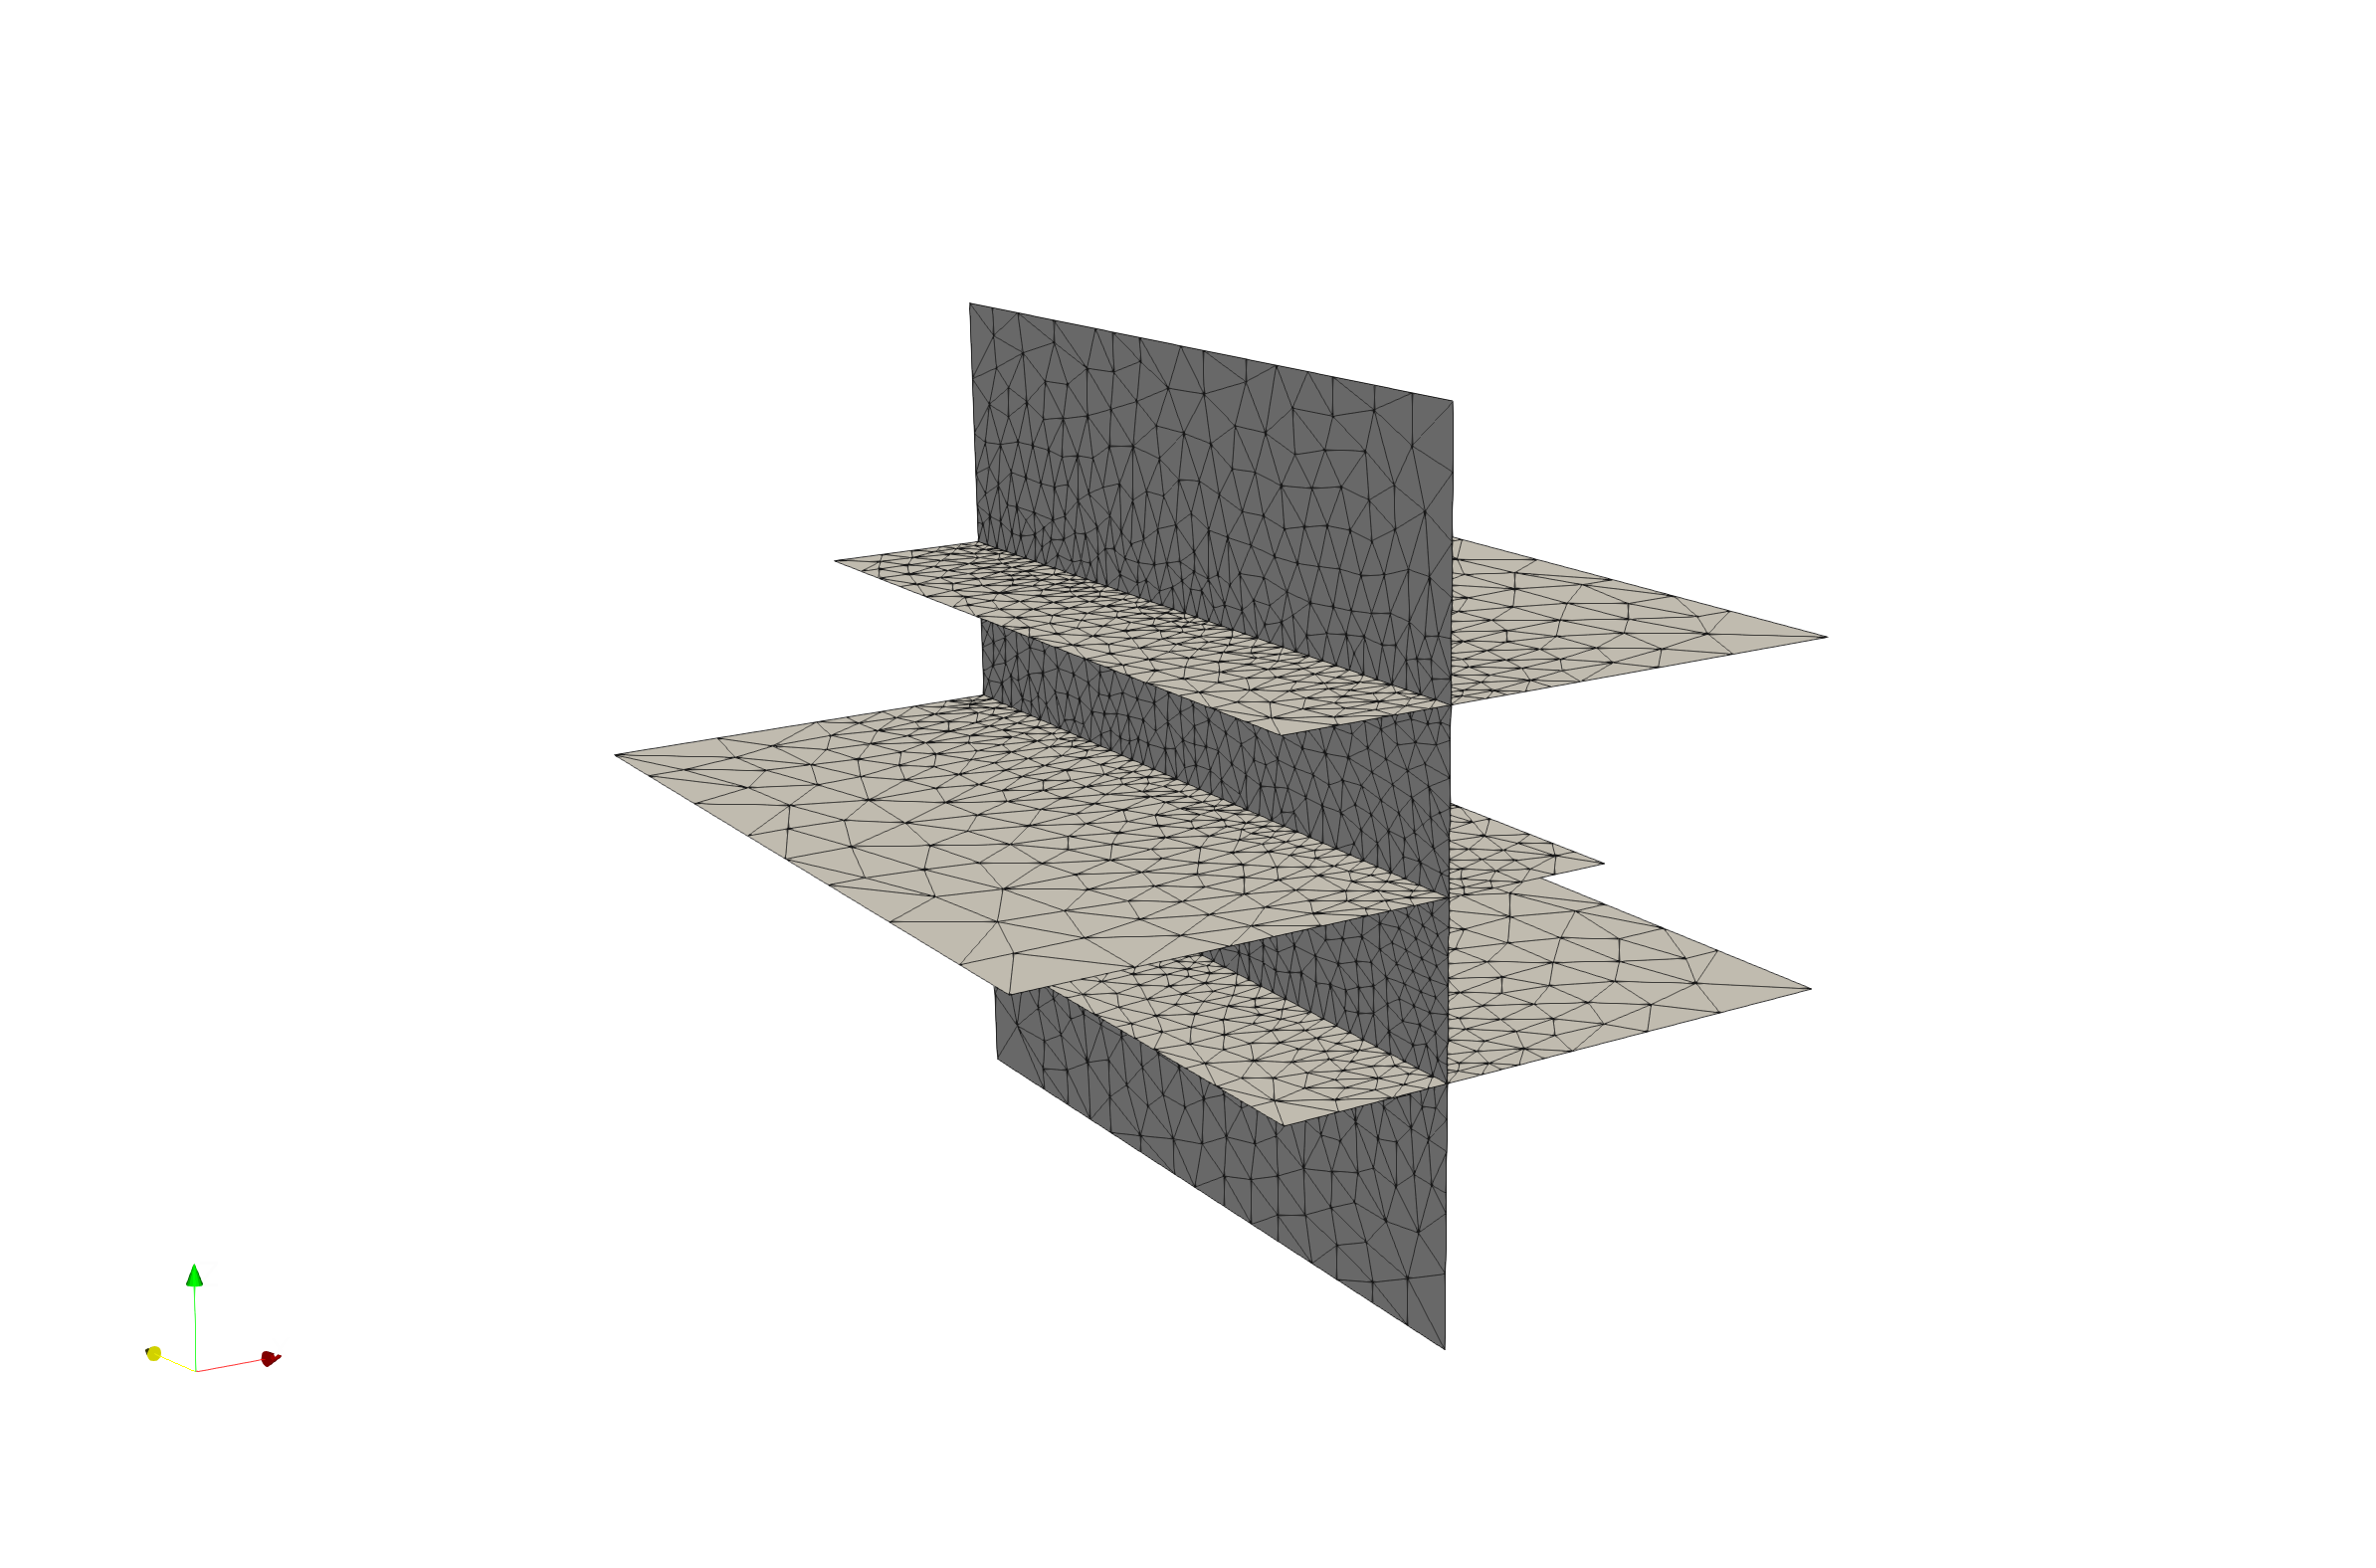
\includegraphics{4_user_rectangles_mesh.png}}\hfill}

The network of four fractures,  colored by pressure solution.
High pressure (red) Dirichlet boundary conditions are applied on the edge of the single fracture along the boundary x = -0.5, and low pressure (blue) boundary conditions are applied on the edges of the two fractures at the boundary x = 0.5.
This image is created by loading the file 4\_user\_defined\_rectangles/PFLOTRAN/parsed\_vtk/dfn\_explicit-001.vtk into Paraview.

{\hfill\scalebox{1.000000}{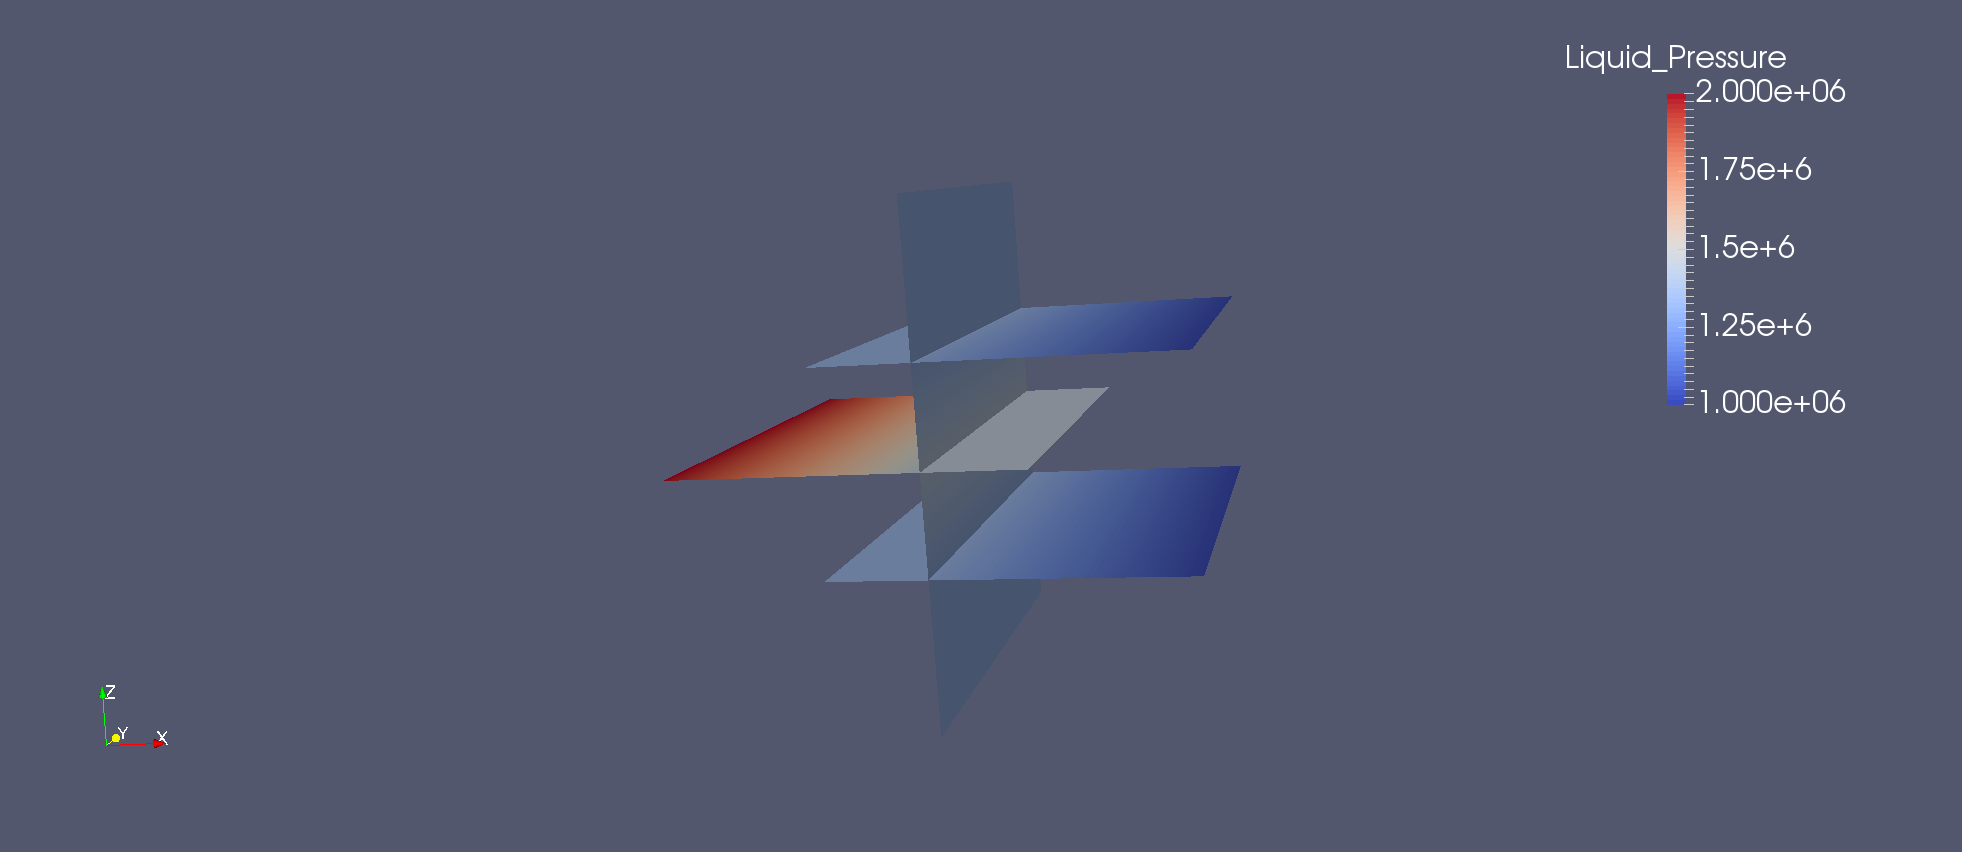
\includegraphics{4_user_rectangles_pressure.png}}\hfill}

Particle trajectories on the network of four fractures.
Particles are inserted uniformly along the inlet fracture on the left side of the image.
Particles exit the domain through the two horizontal fractures on the right side of the image.
Due to the stochastic nature of the particle tracking algorithm, your pathlines might not be exactly the same as in this image.
Trajectories are colored by the current velocity magnitude of the particle's velocity.
Trajectories can be visualized by loading the files part\_*.inp, in the folder 4\_user\_rectangles/dfnTrans/trajectories/
We have used the extract surface and tube filters in paraview for visual clarity.

{\hfill\scalebox{1.000000}{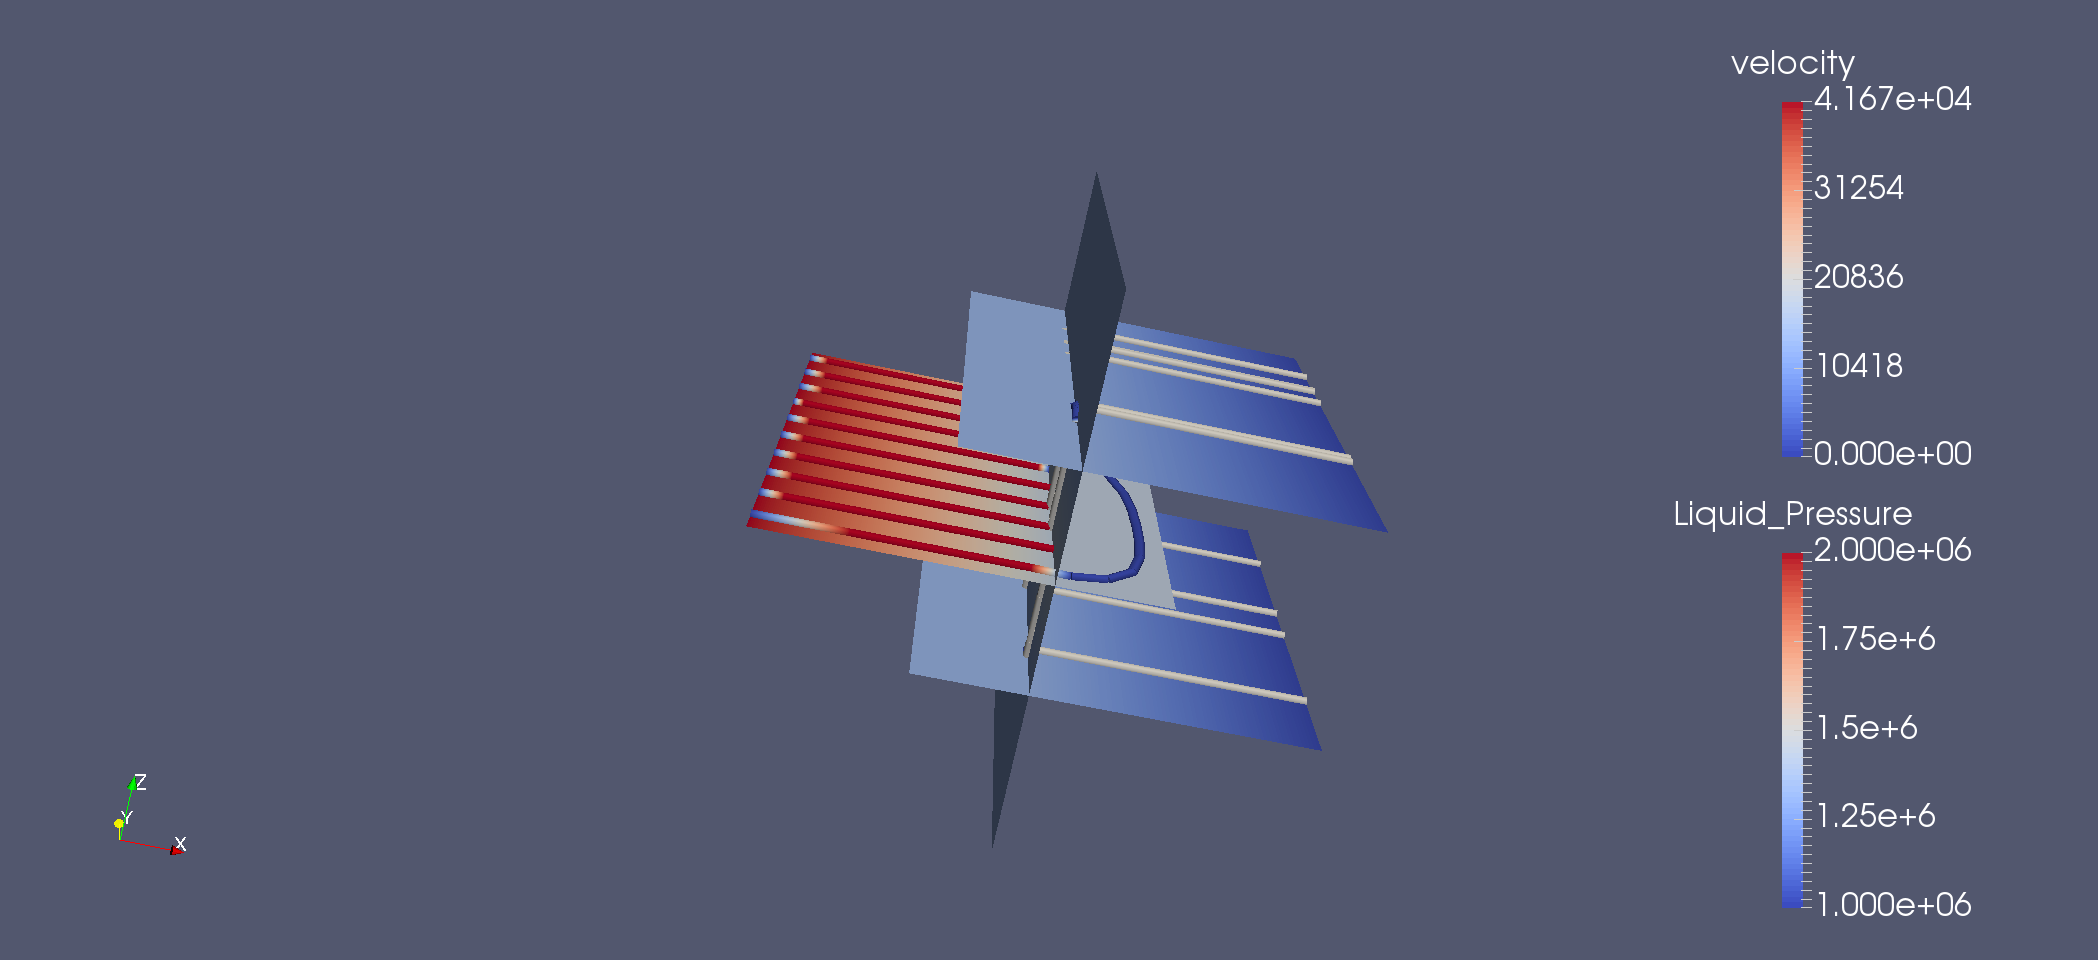
\includegraphics{4_user_rectangles_trace.png}}\hfill}

In the other tests, only a brief description and pictures are provided.


\section{4\_user\_defined\_ellipses}
\label{examples:user-defined-ellipses}
This test case consists of four user defined elliptical fractures within a a cubic domain with sides of length one meter. In this case the ellipses are approximated using 5 vertices. The input file specifiying the ellipses is in dfnWorks-Version2.0/tests, and is named define\_4\_user\_ellipses.dat.

{\hfill\scalebox{1.000000}{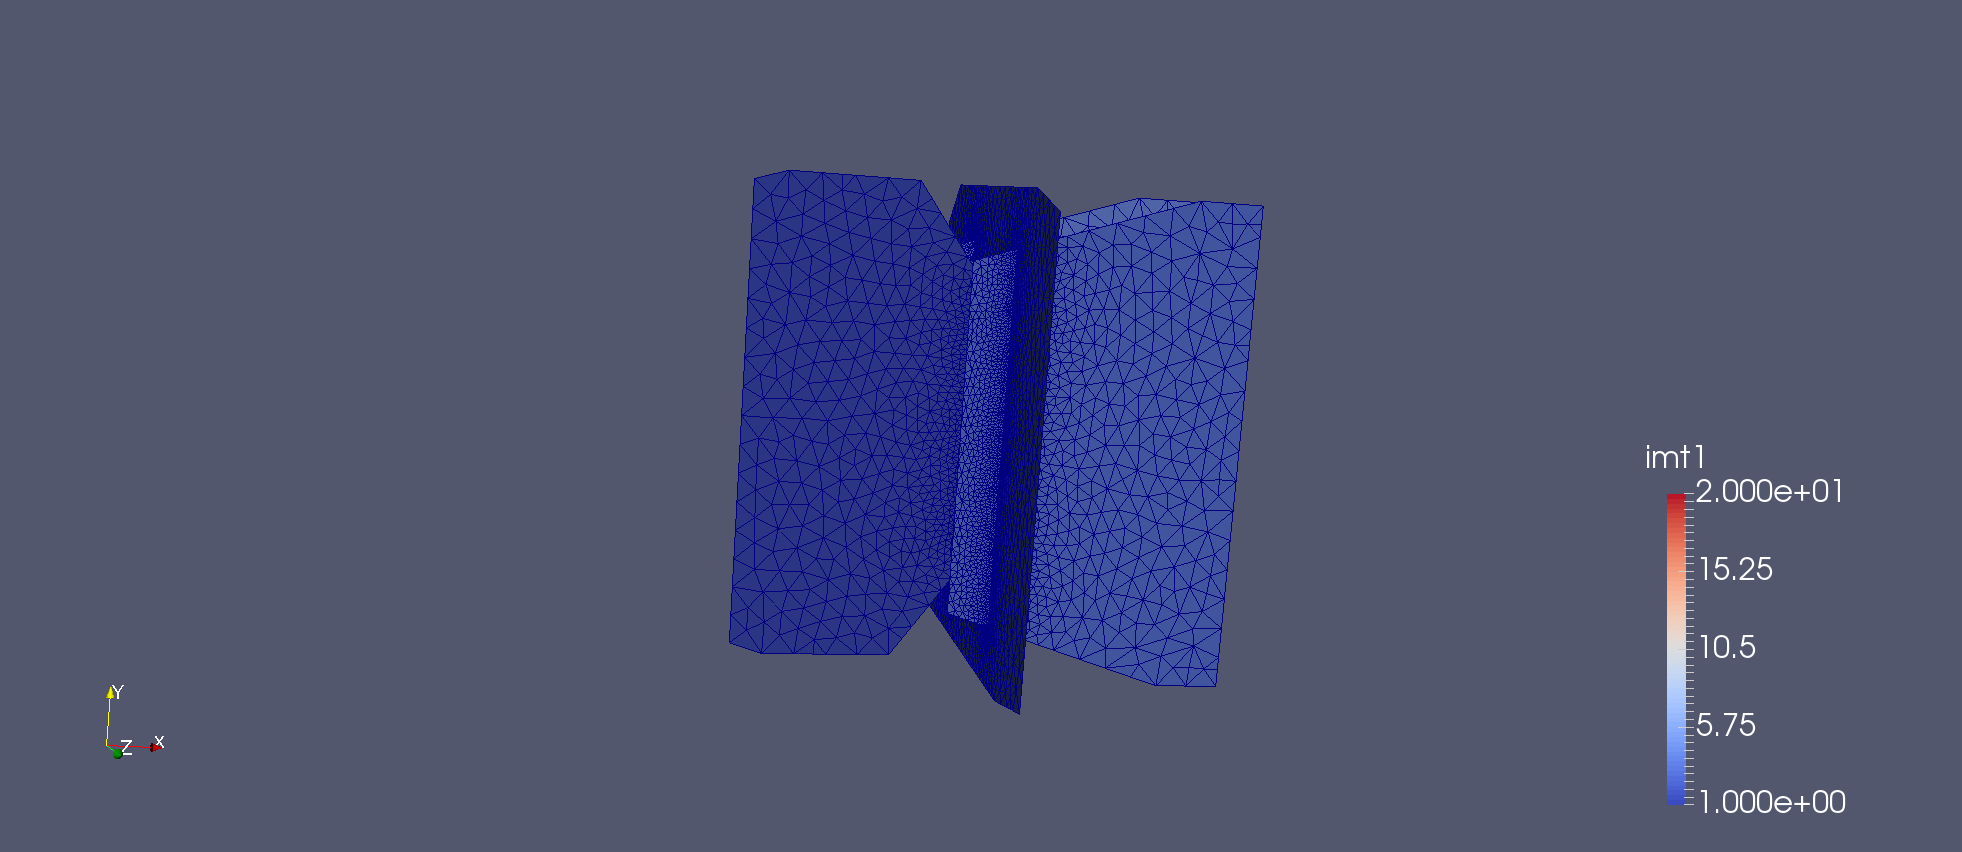
\includegraphics{4_user_ellipses_mesh.png}}\hfill}

\begin{DUlineblock}{0em}
\item[] 
\item[] 
\end{DUlineblock}

{\hfill\scalebox{1.000000}{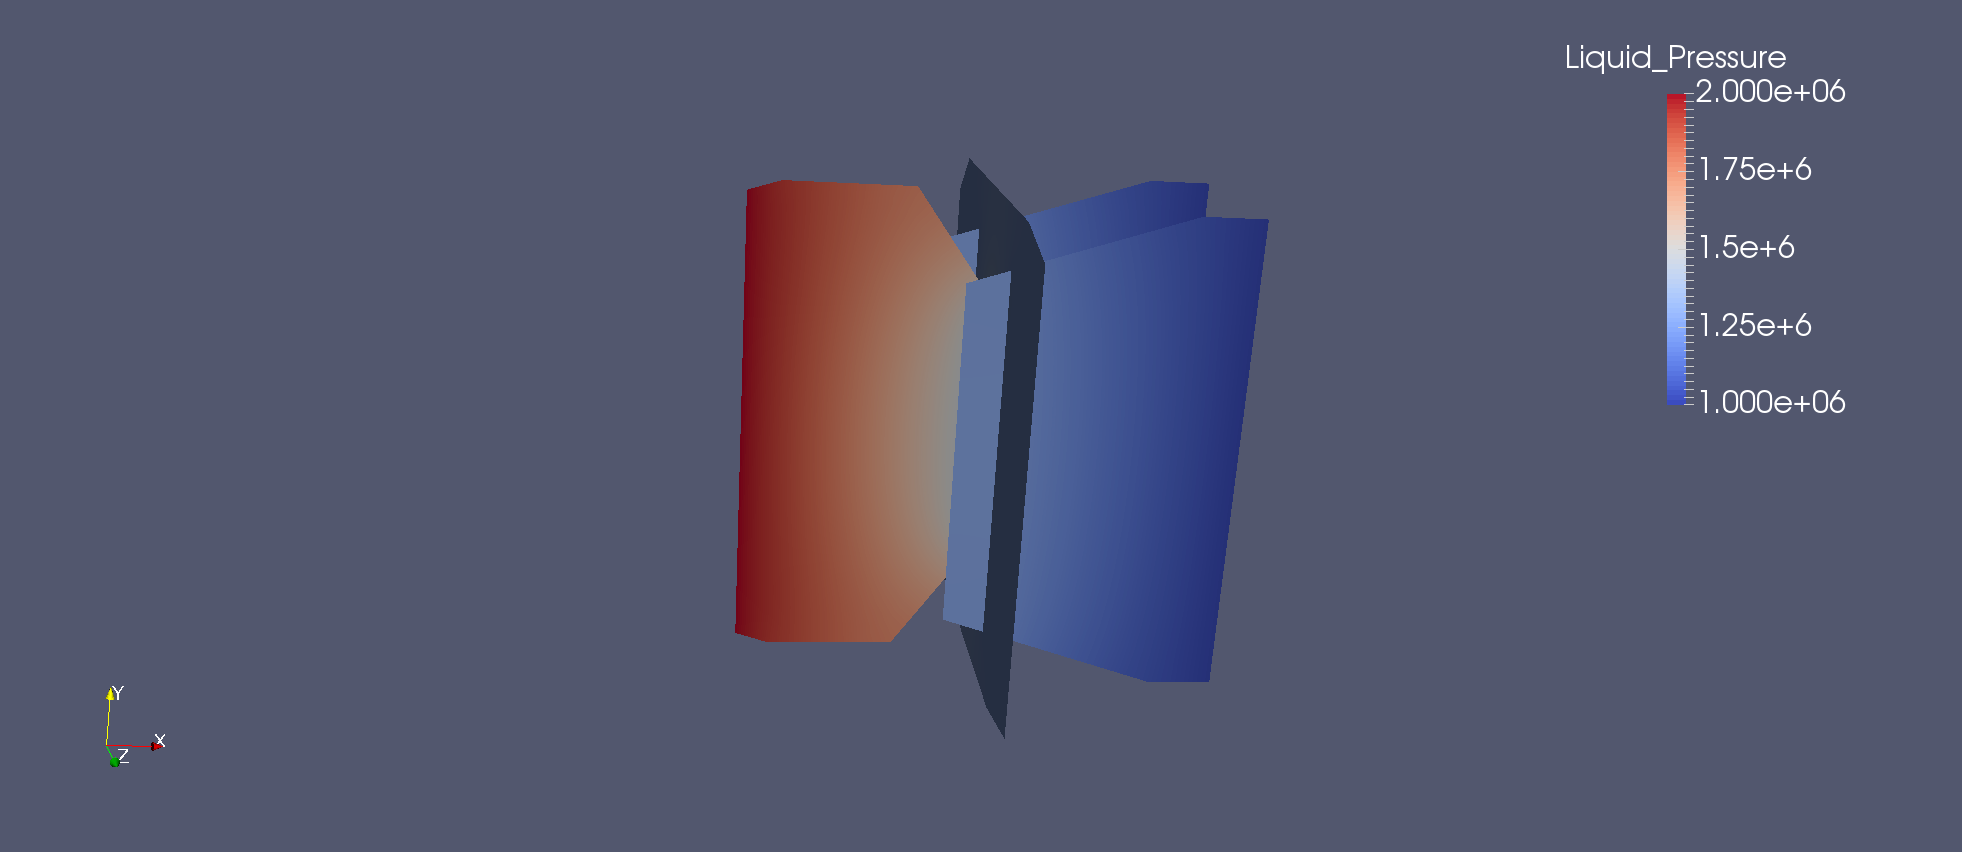
\includegraphics{4_user_ellipses_pressure.png}}\hfill}

\begin{DUlineblock}{0em}
\item[] 
\item[] 
\end{DUlineblock}

{\hfill\scalebox{1.000000}{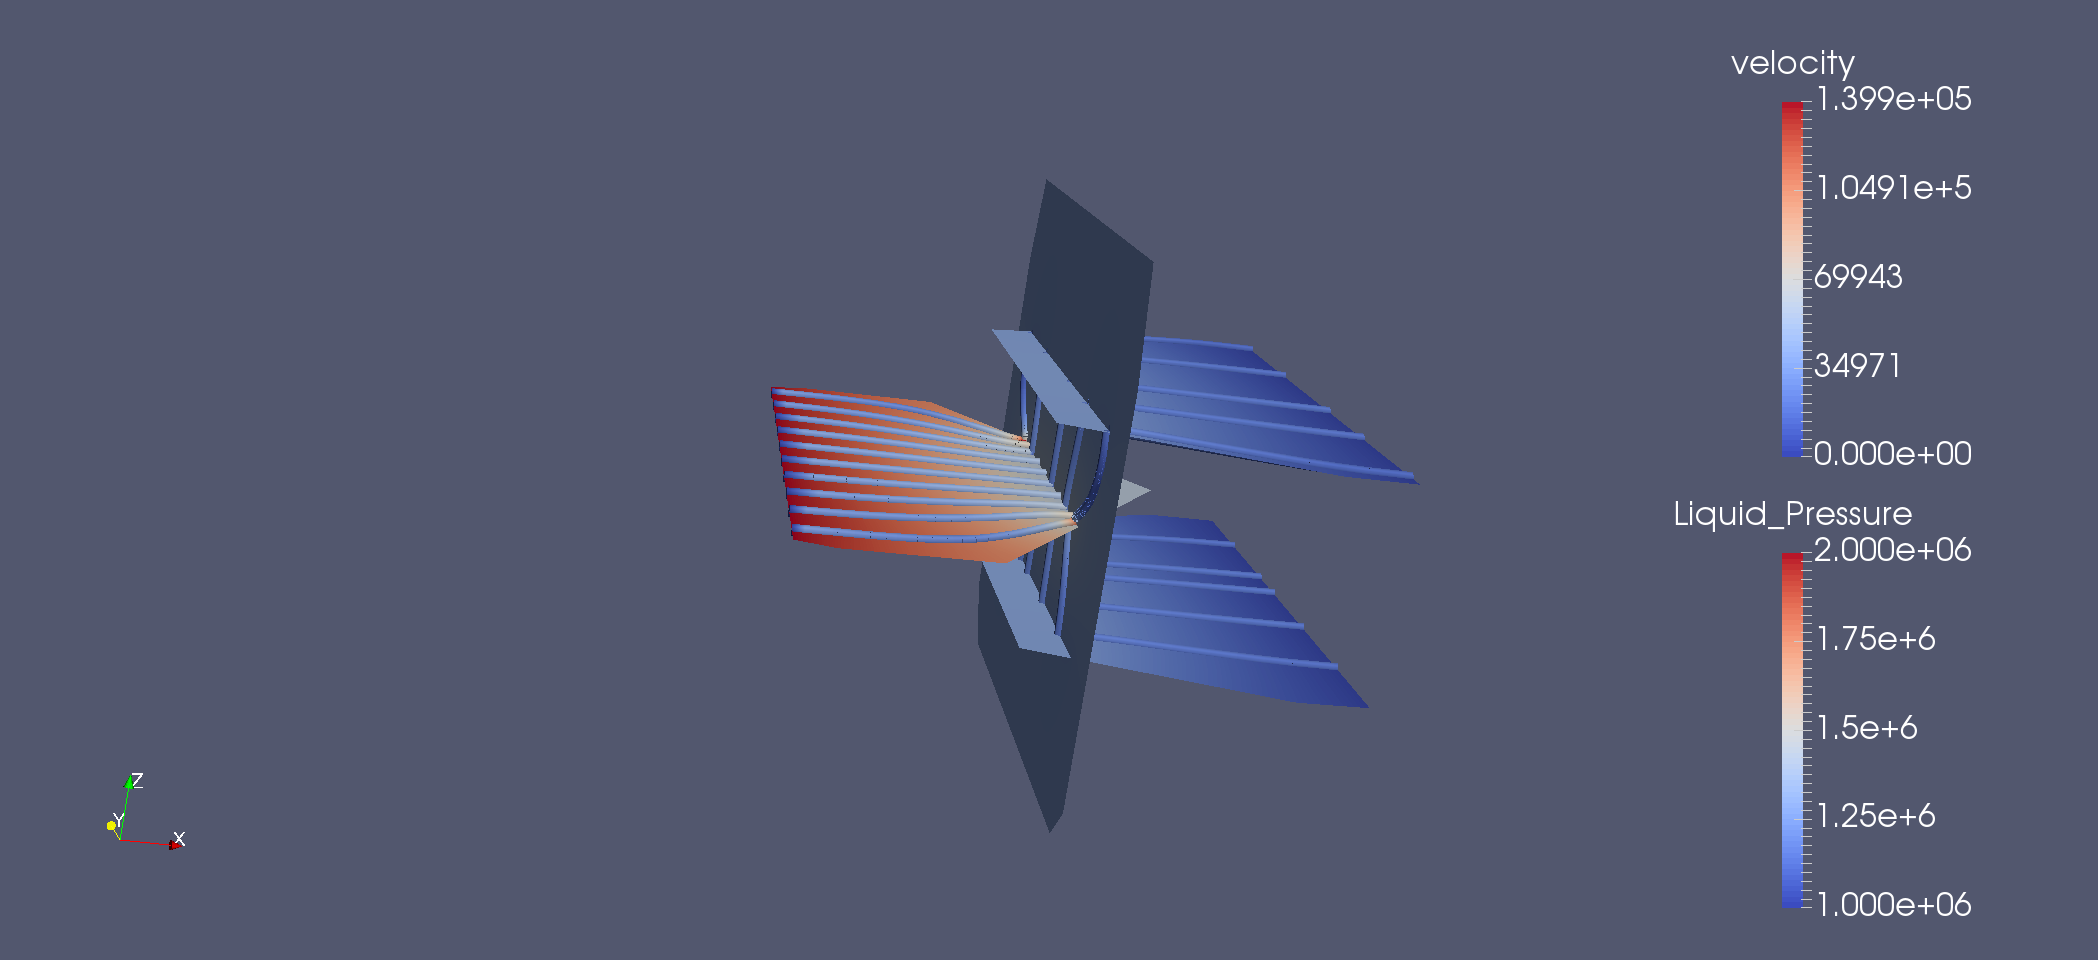
\includegraphics{4_user_ellipses_trace.png}}\hfill}

\begin{DUlineblock}{0em}
\item[] 
\item[] 
\end{DUlineblock}


\section{truncated\_power\_law\_dist}
\label{examples:truncated-power-law-dist}
This test case consists of two families whose sizes have a truncated power law distribution with a minimum size of 0.5m and a maximum size of 50m. The domain size is cubic with an edge length of 4m. The other input parameters can be found in tests/gen\_truncated\_power\_law\_dist.dat.

{\hfill\scalebox{1.000000}{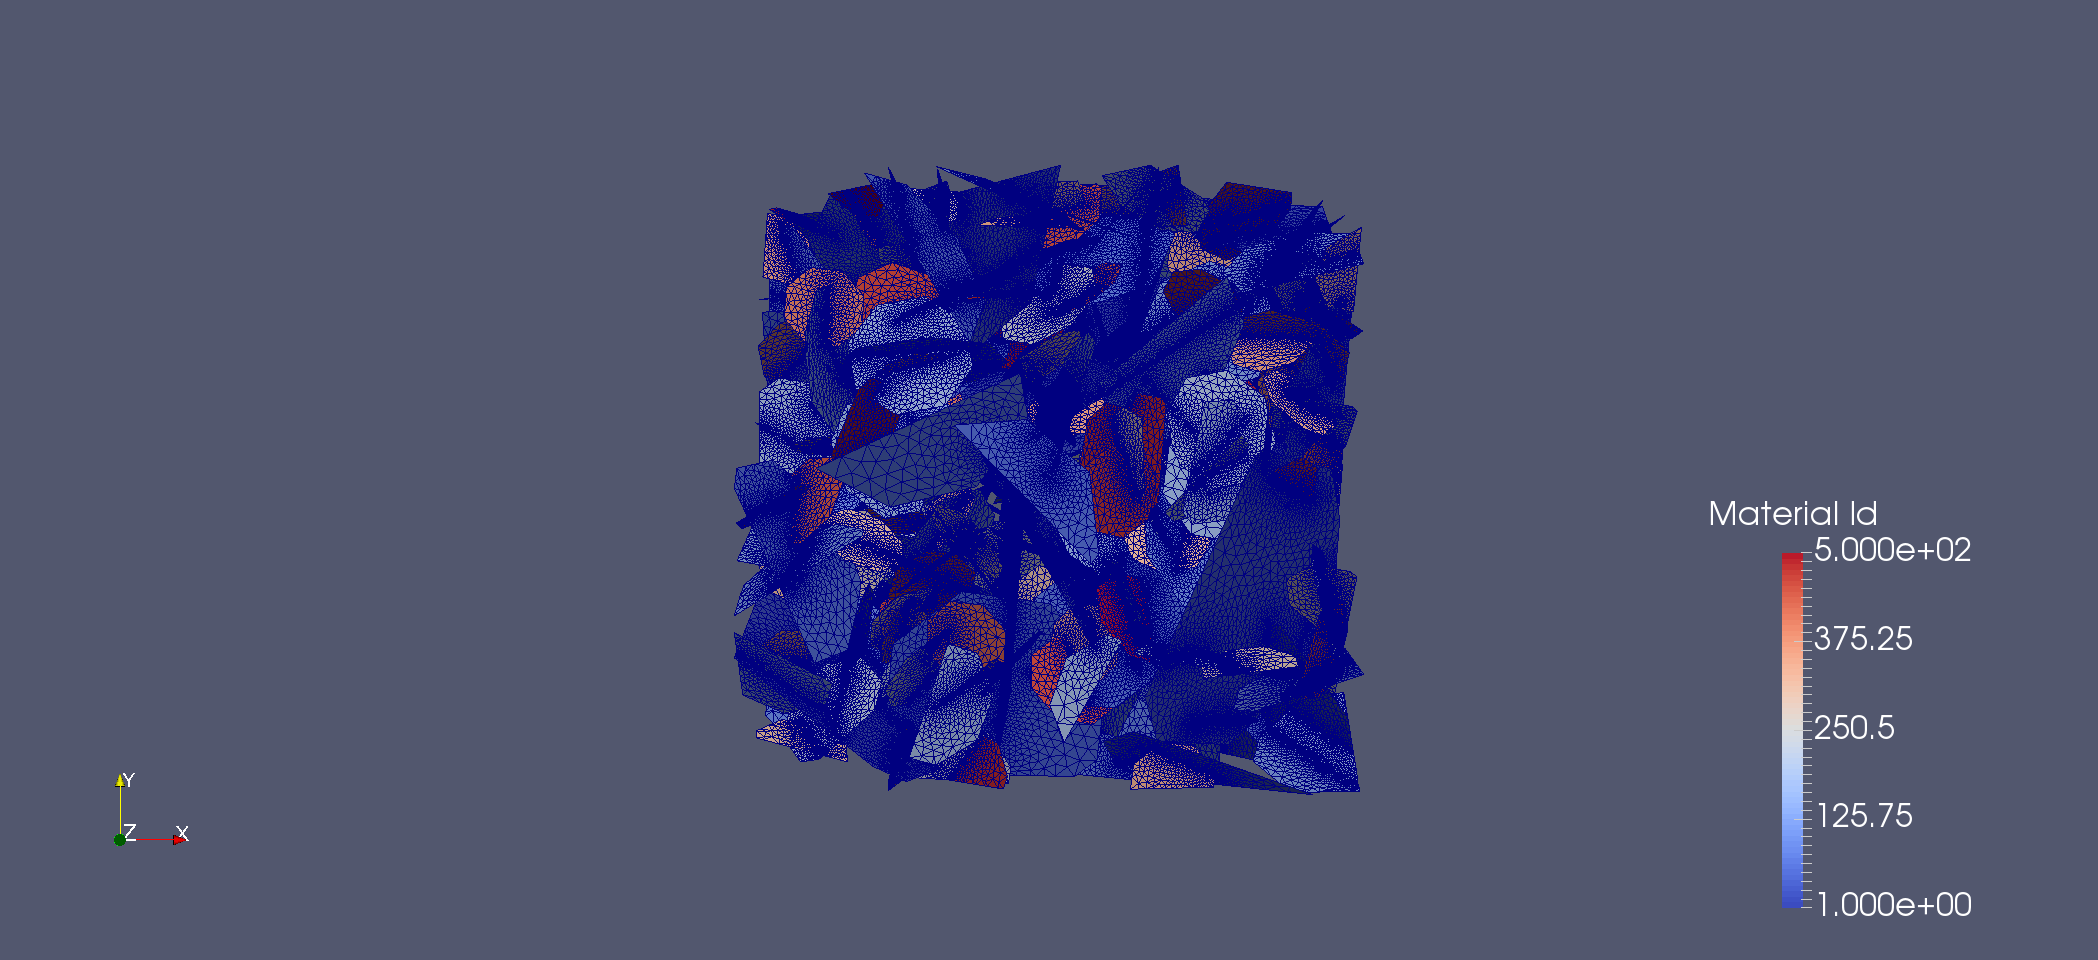
\includegraphics{power_mesh.png}}\hfill}

\begin{DUlineblock}{0em}
\item[] 
\item[] 
\end{DUlineblock}

{\hfill\scalebox{1.000000}{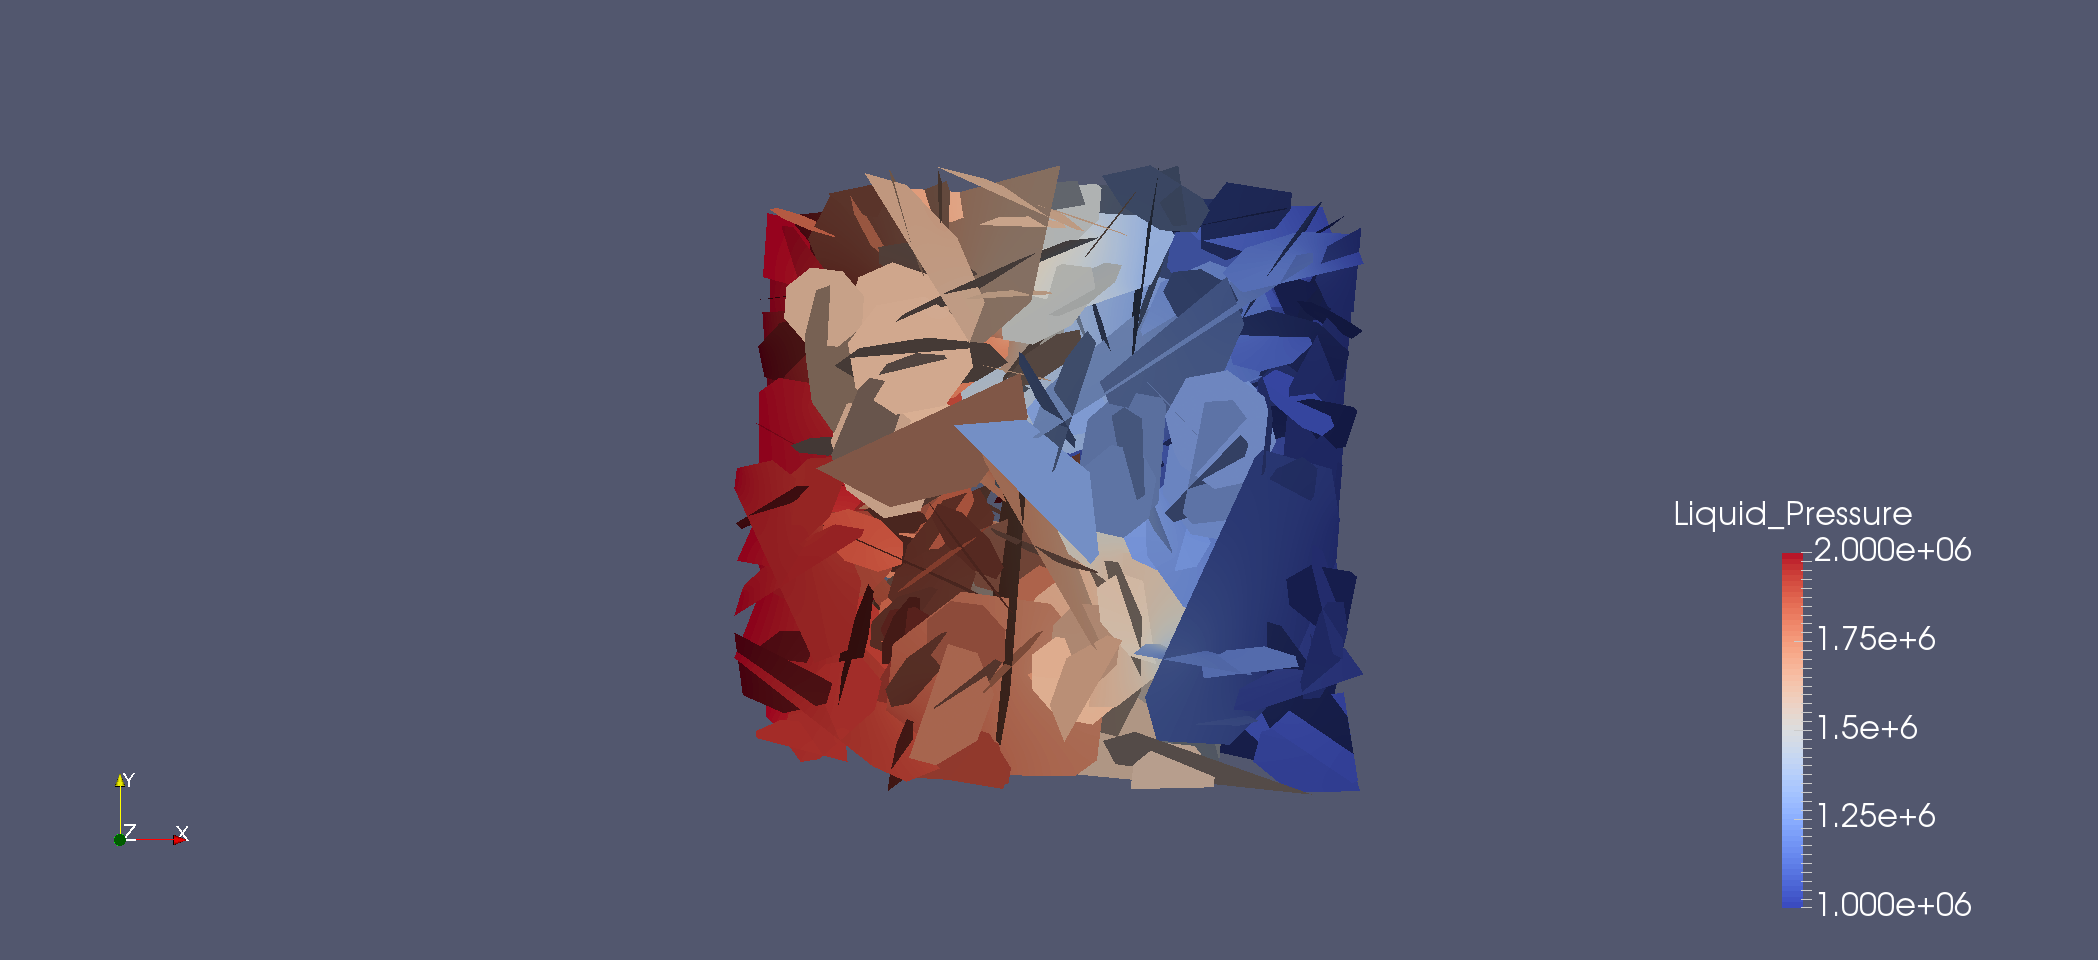
\includegraphics{power_pressure.png}}\hfill}

\begin{DUlineblock}{0em}
\item[] 
\item[] 
\end{DUlineblock}

{\hfill\scalebox{1.000000}{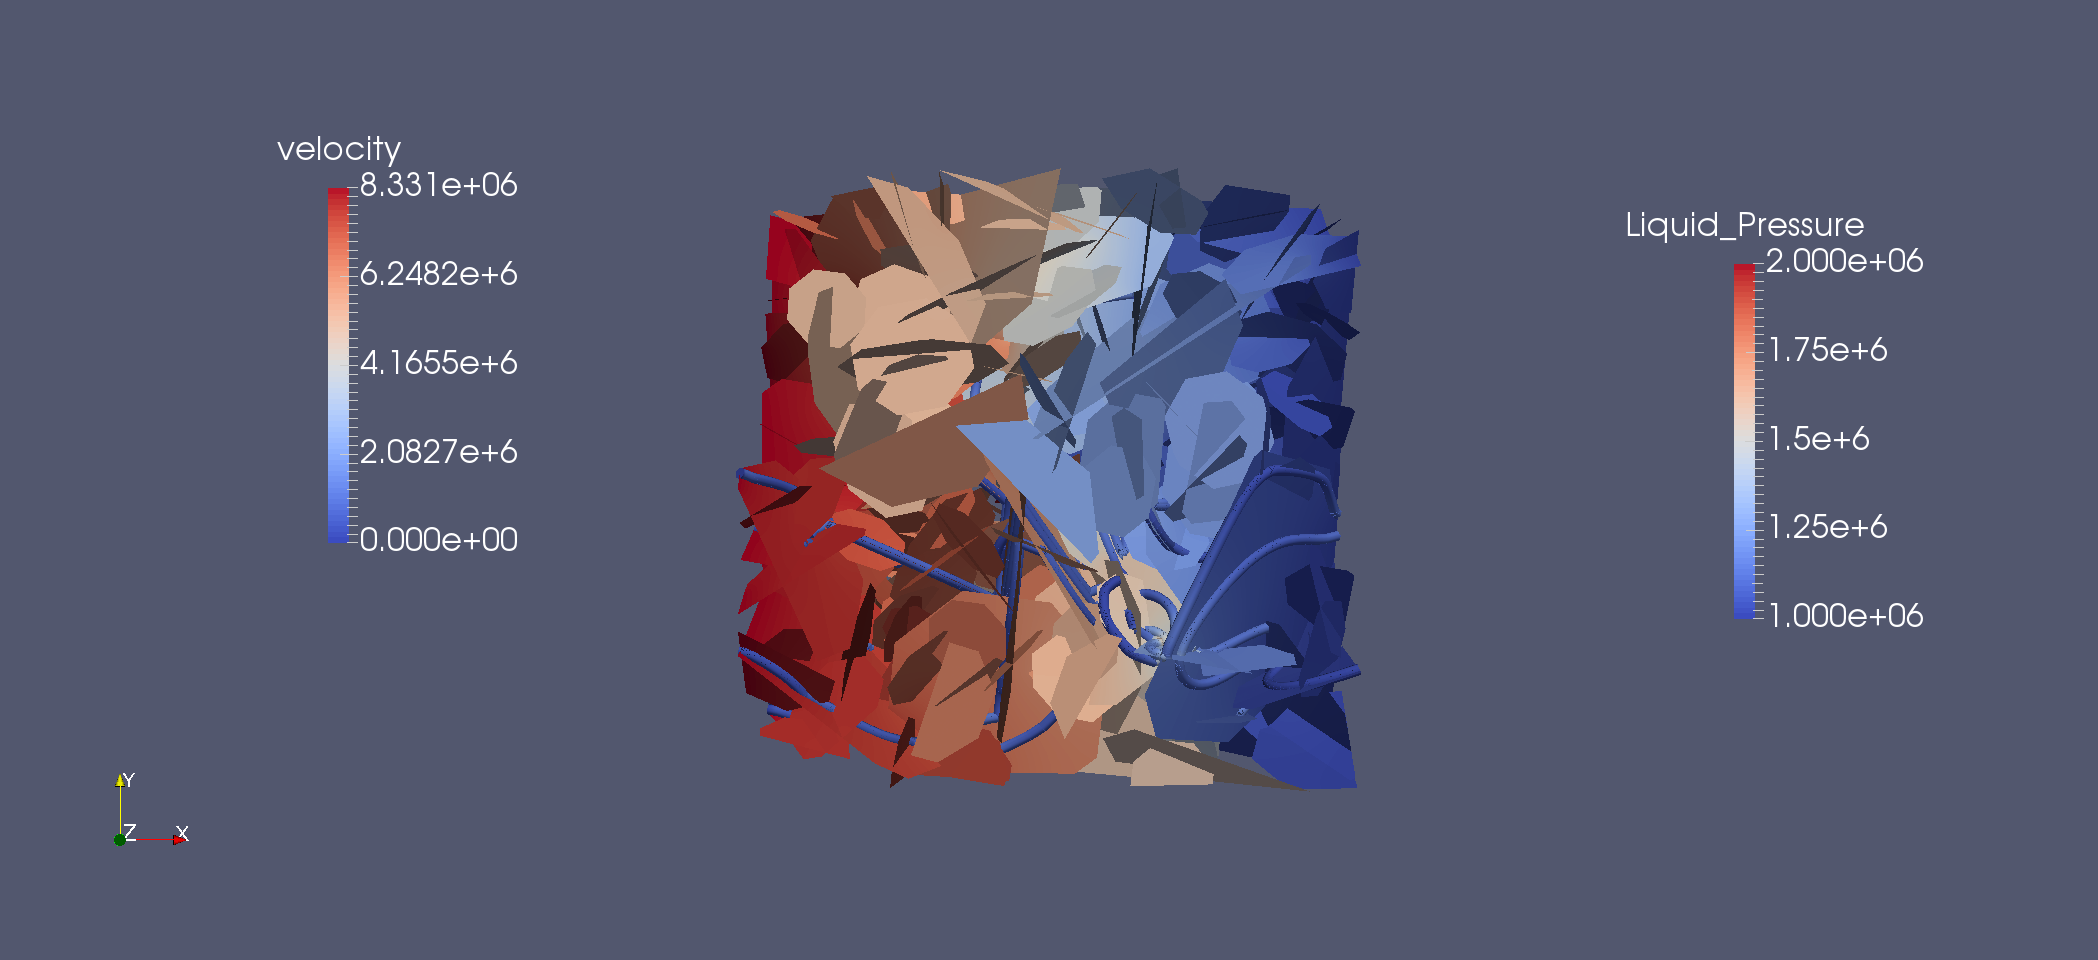
\includegraphics{power_trace.png}}\hfill}


\section{exponential\_dist}
\label{examples:exponential-dist}
This test case consists of a family of fractures whose size is exponentially distributed with a minimum size of 1m and a maximum size of 50m. The domain is cubic with an edge length of 10m. All input parameters for the generator can be found in tests/gen\_exponential\_dist.dat.

{\hfill\scalebox{1.000000}{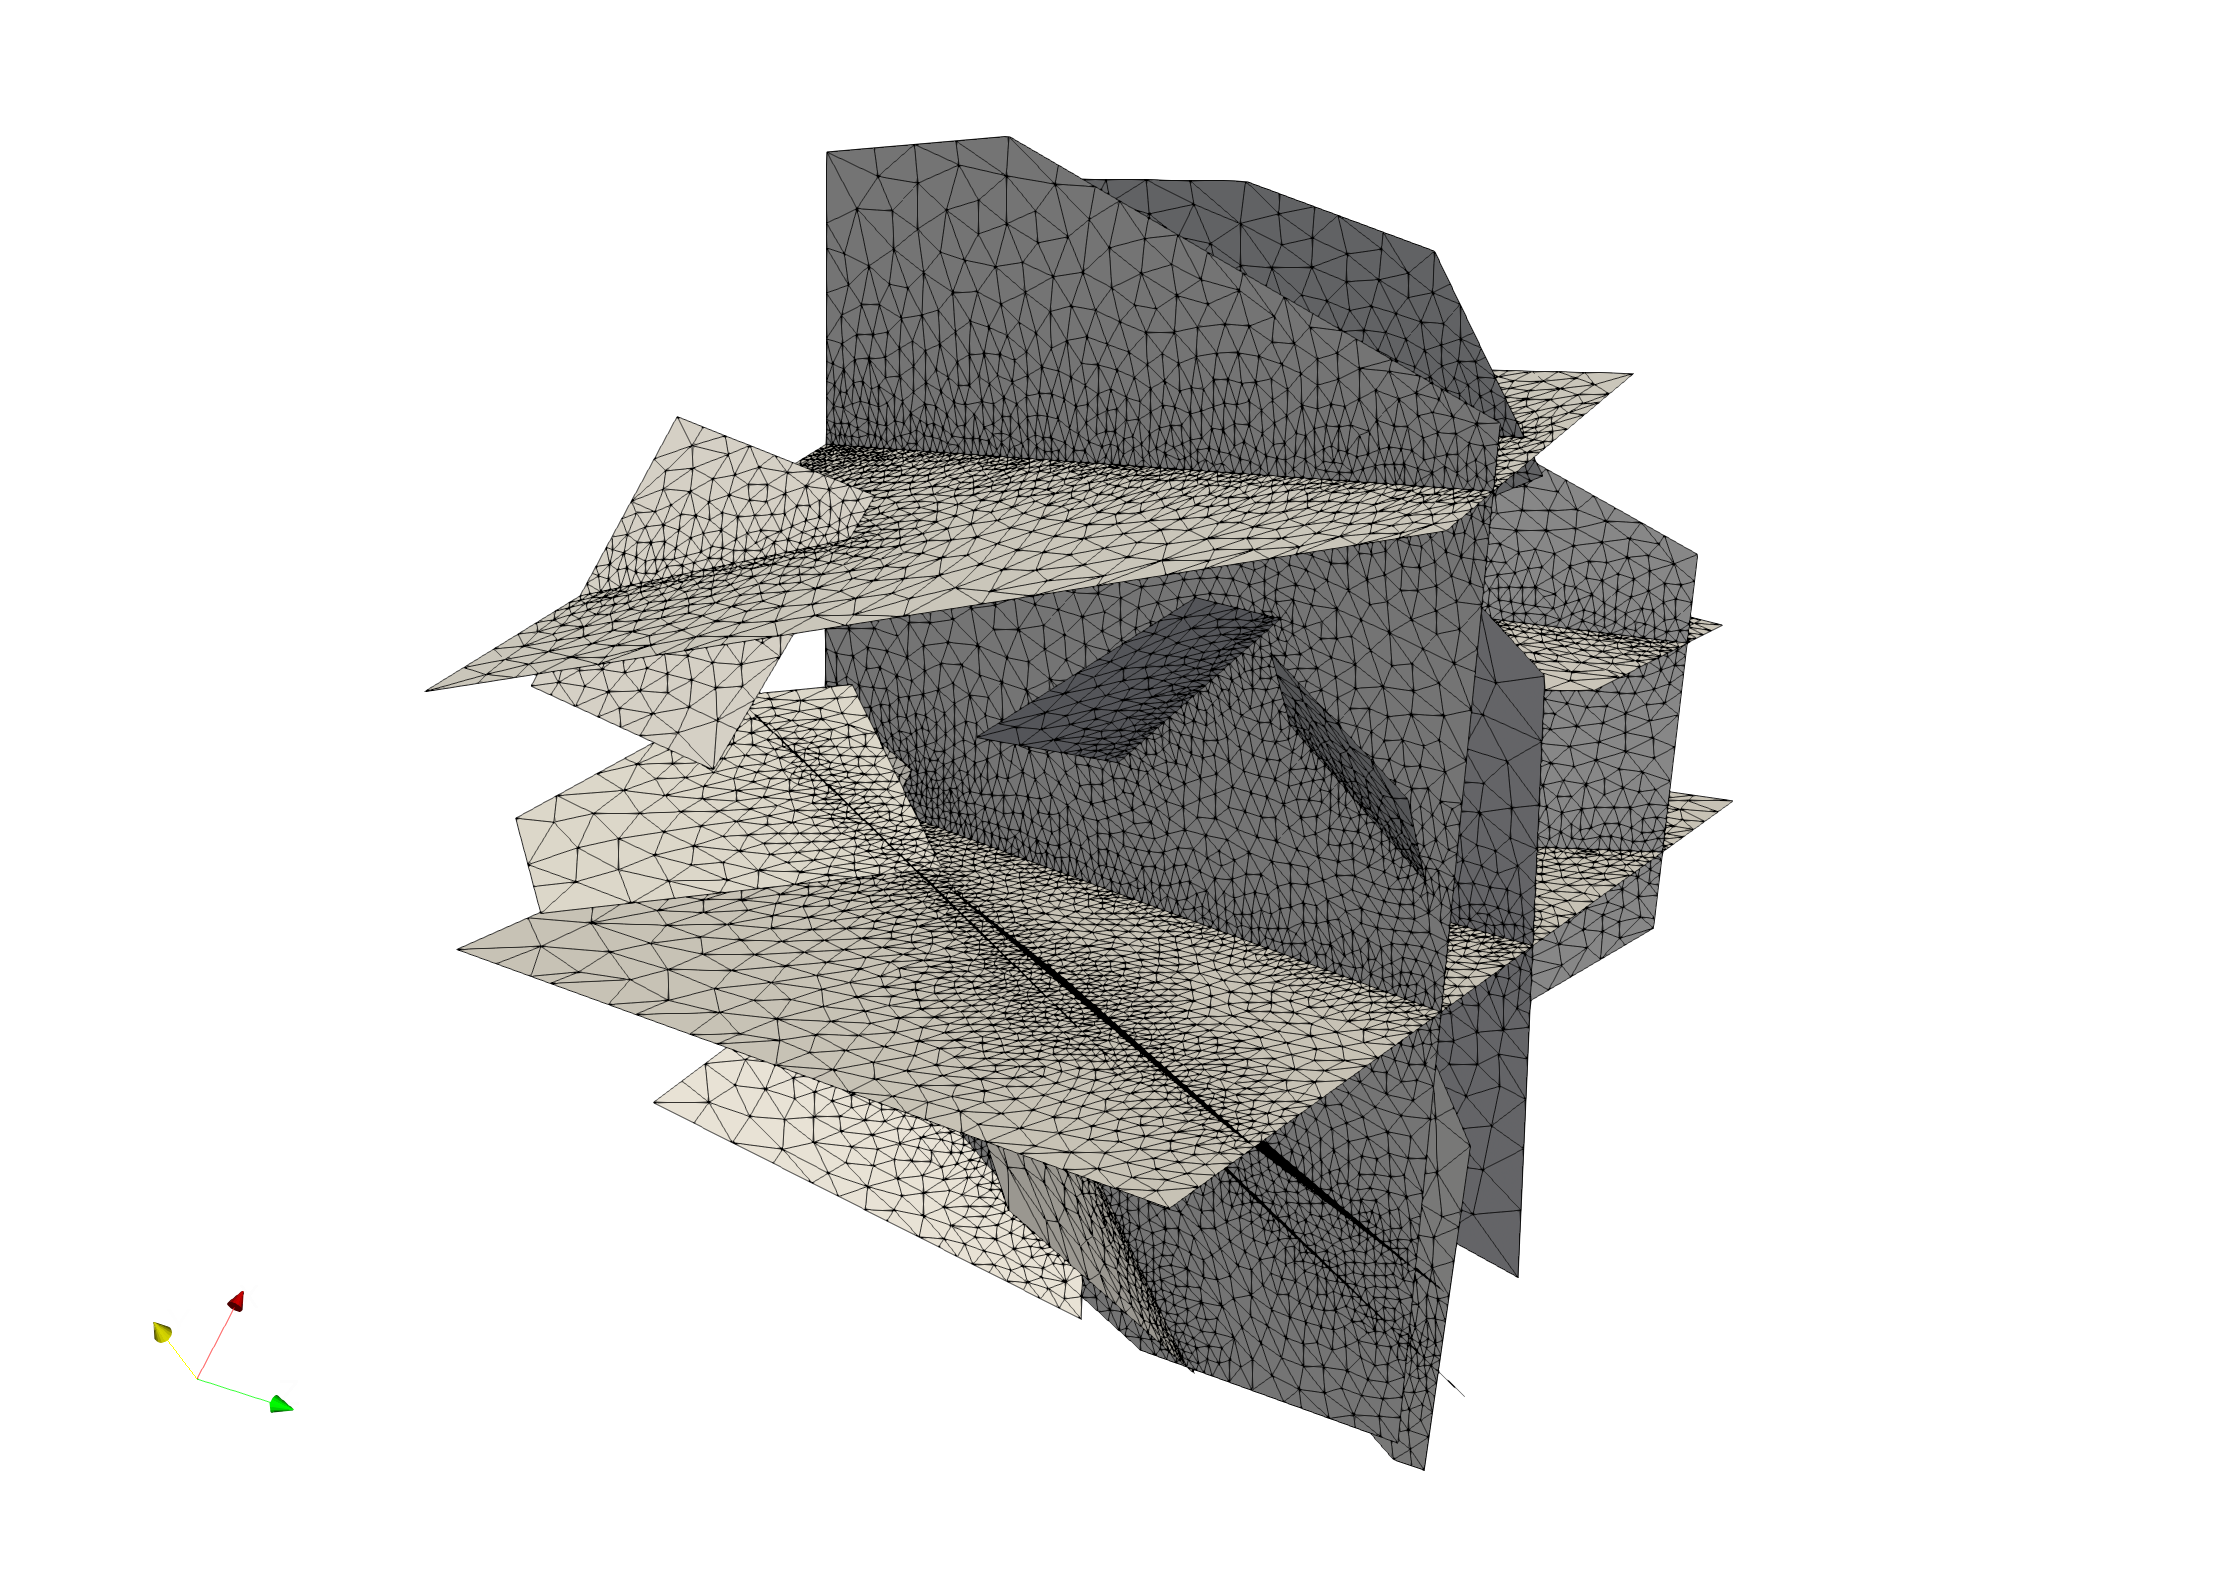
\includegraphics{exp_mesh.png}}\hfill}

\begin{DUlineblock}{0em}
\item[] 
\item[] 
\end{DUlineblock}

{\hfill\scalebox{1.000000}{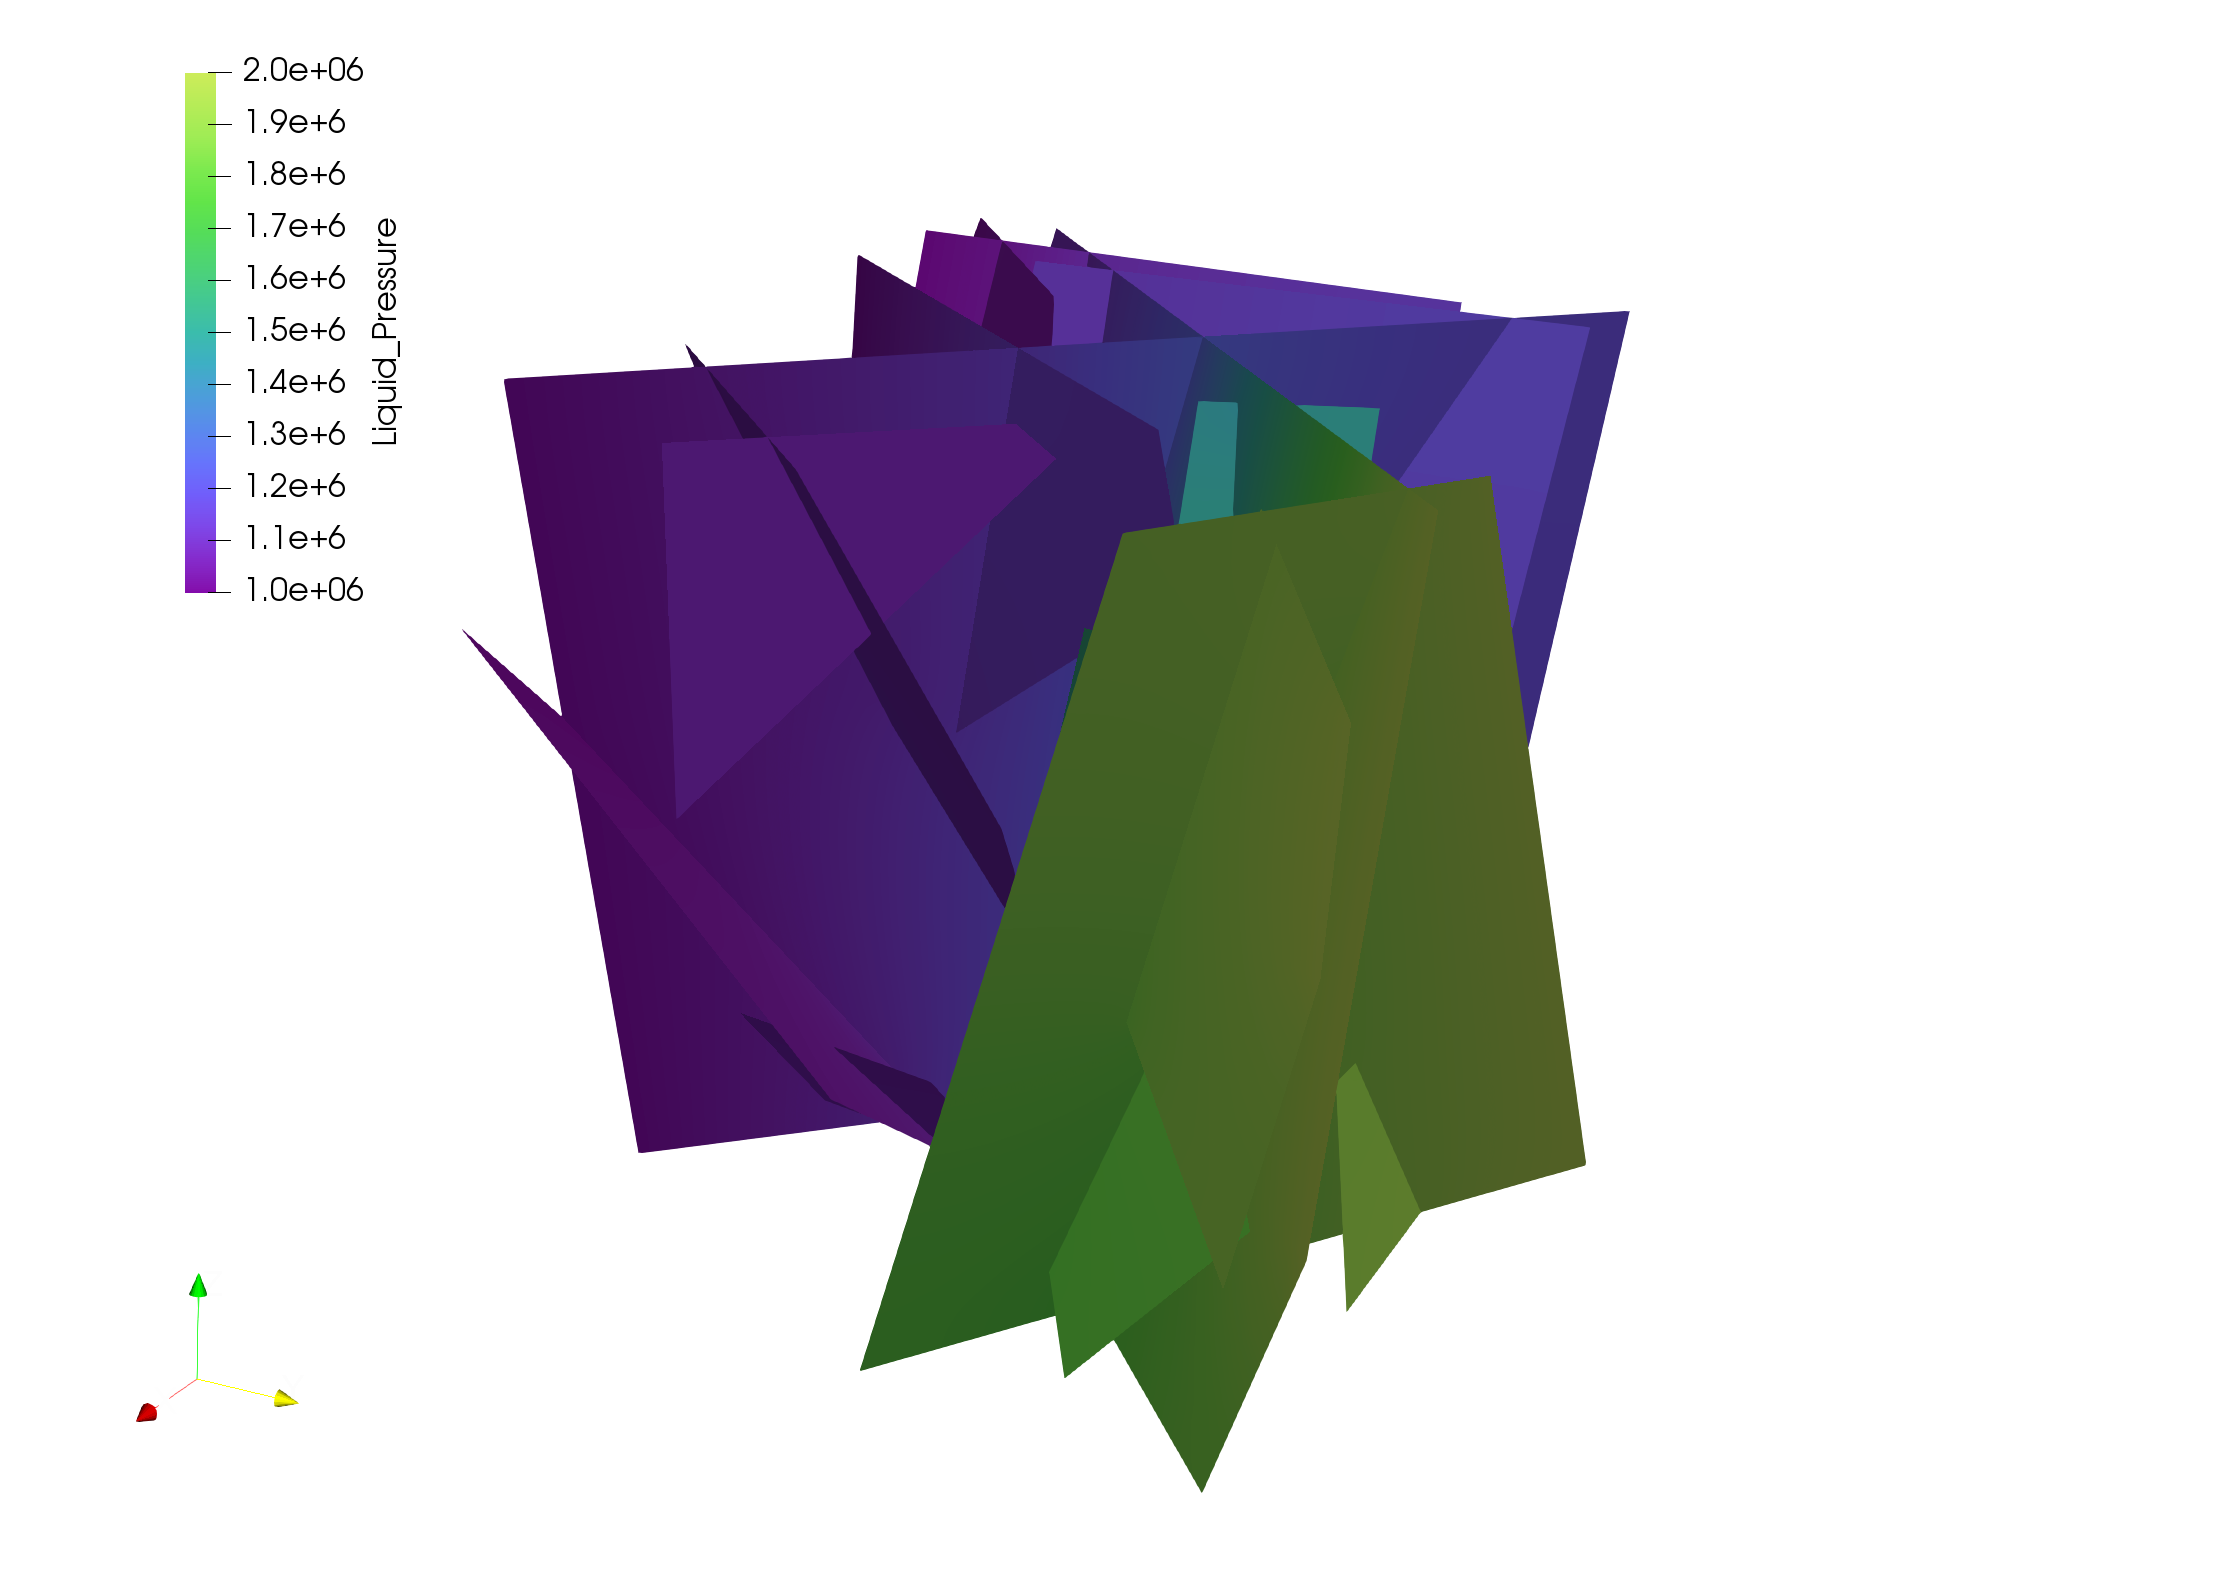
\includegraphics{exp_pressure.png}}\hfill}

\begin{DUlineblock}{0em}
\item[] 
\item[] 
\end{DUlineblock}

{\hfill\scalebox{1.000000}{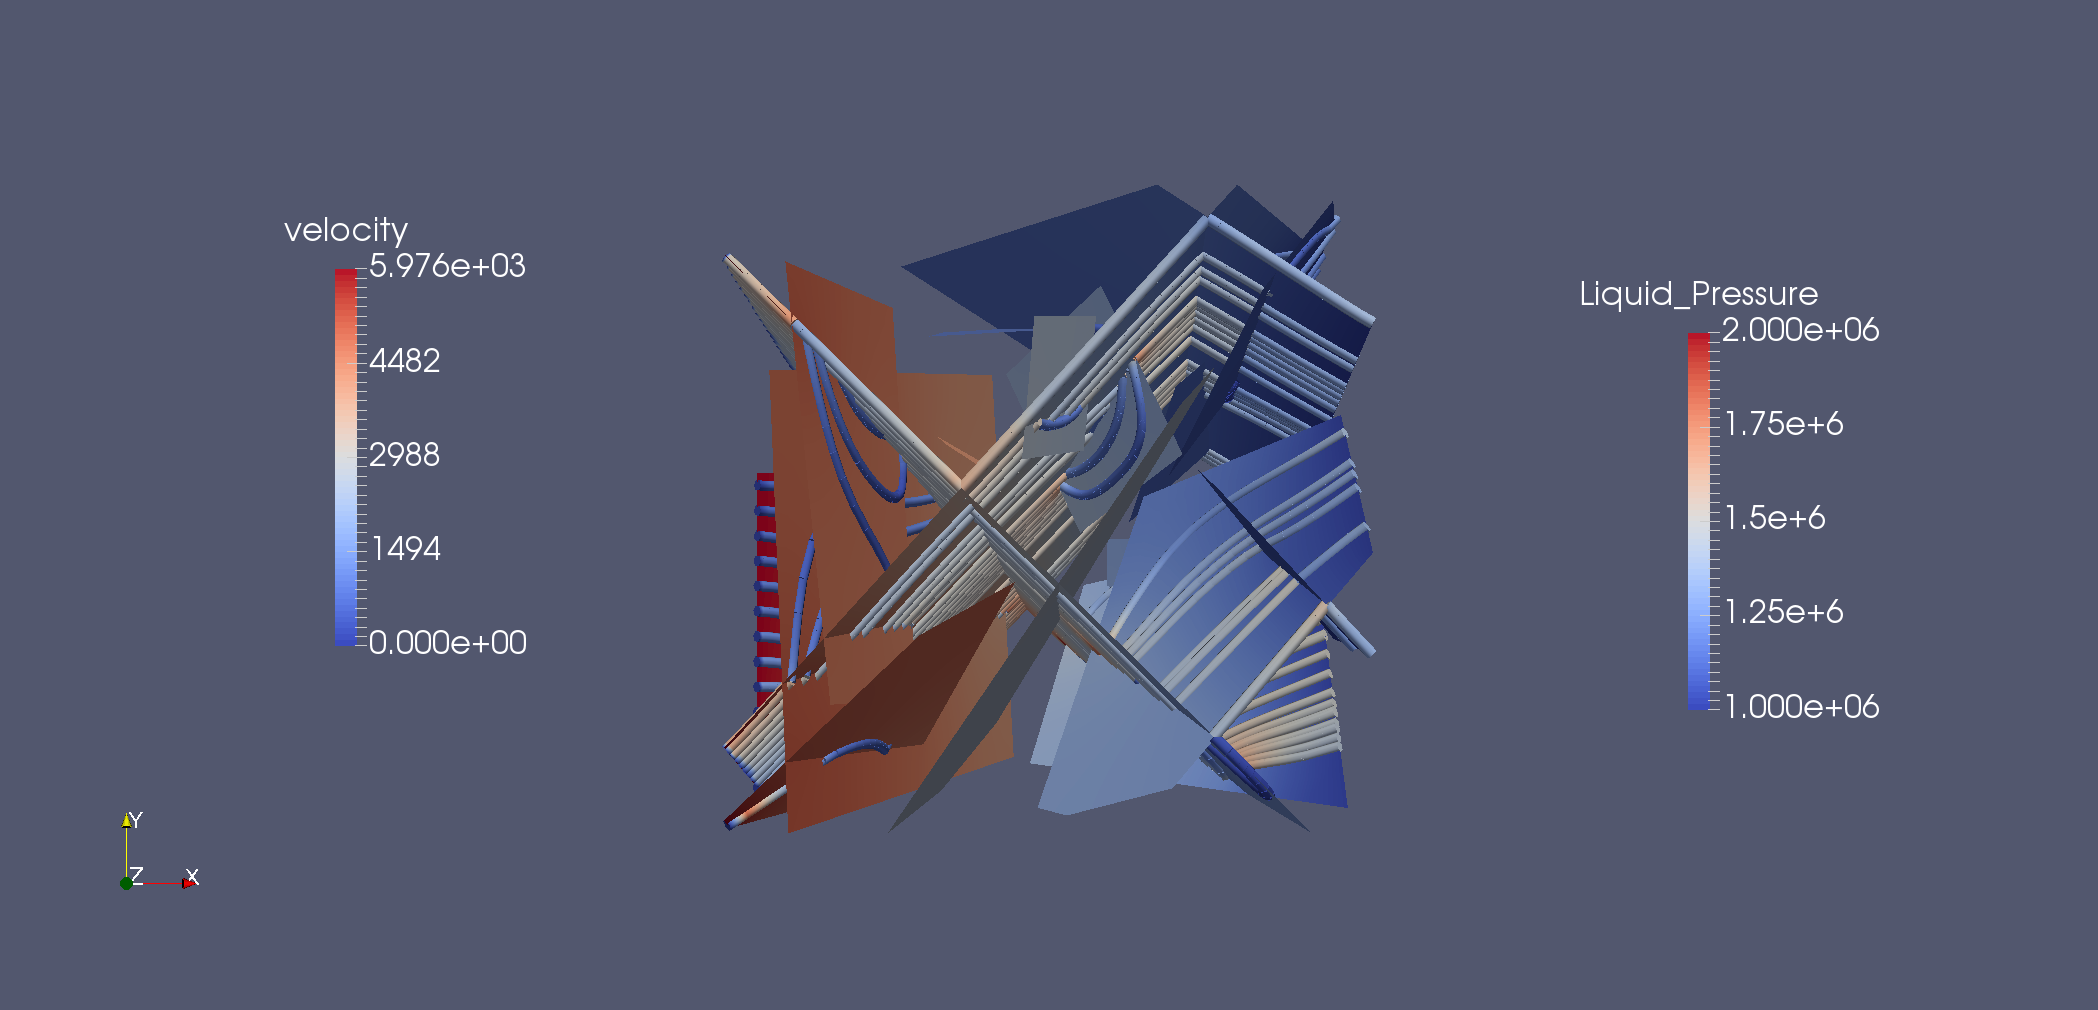
\includegraphics{exp_trace.png}}\hfill}

\begin{DUlineblock}{0em}
\item[] 
\item[] 
\end{DUlineblock}


\section{lognormal\_dist}
\label{examples:lognormal-dist}
This test case consists of two fracture families whose sizes have a lognormal distribution with a minimum size of 0.5m and a maximum size of 50m. The domain size is cubic with an edge length of 10m. All input parameters for the generator can be found in tests/gen\_lognormal\_dist.dat.

{\hfill\scalebox{1.000000}{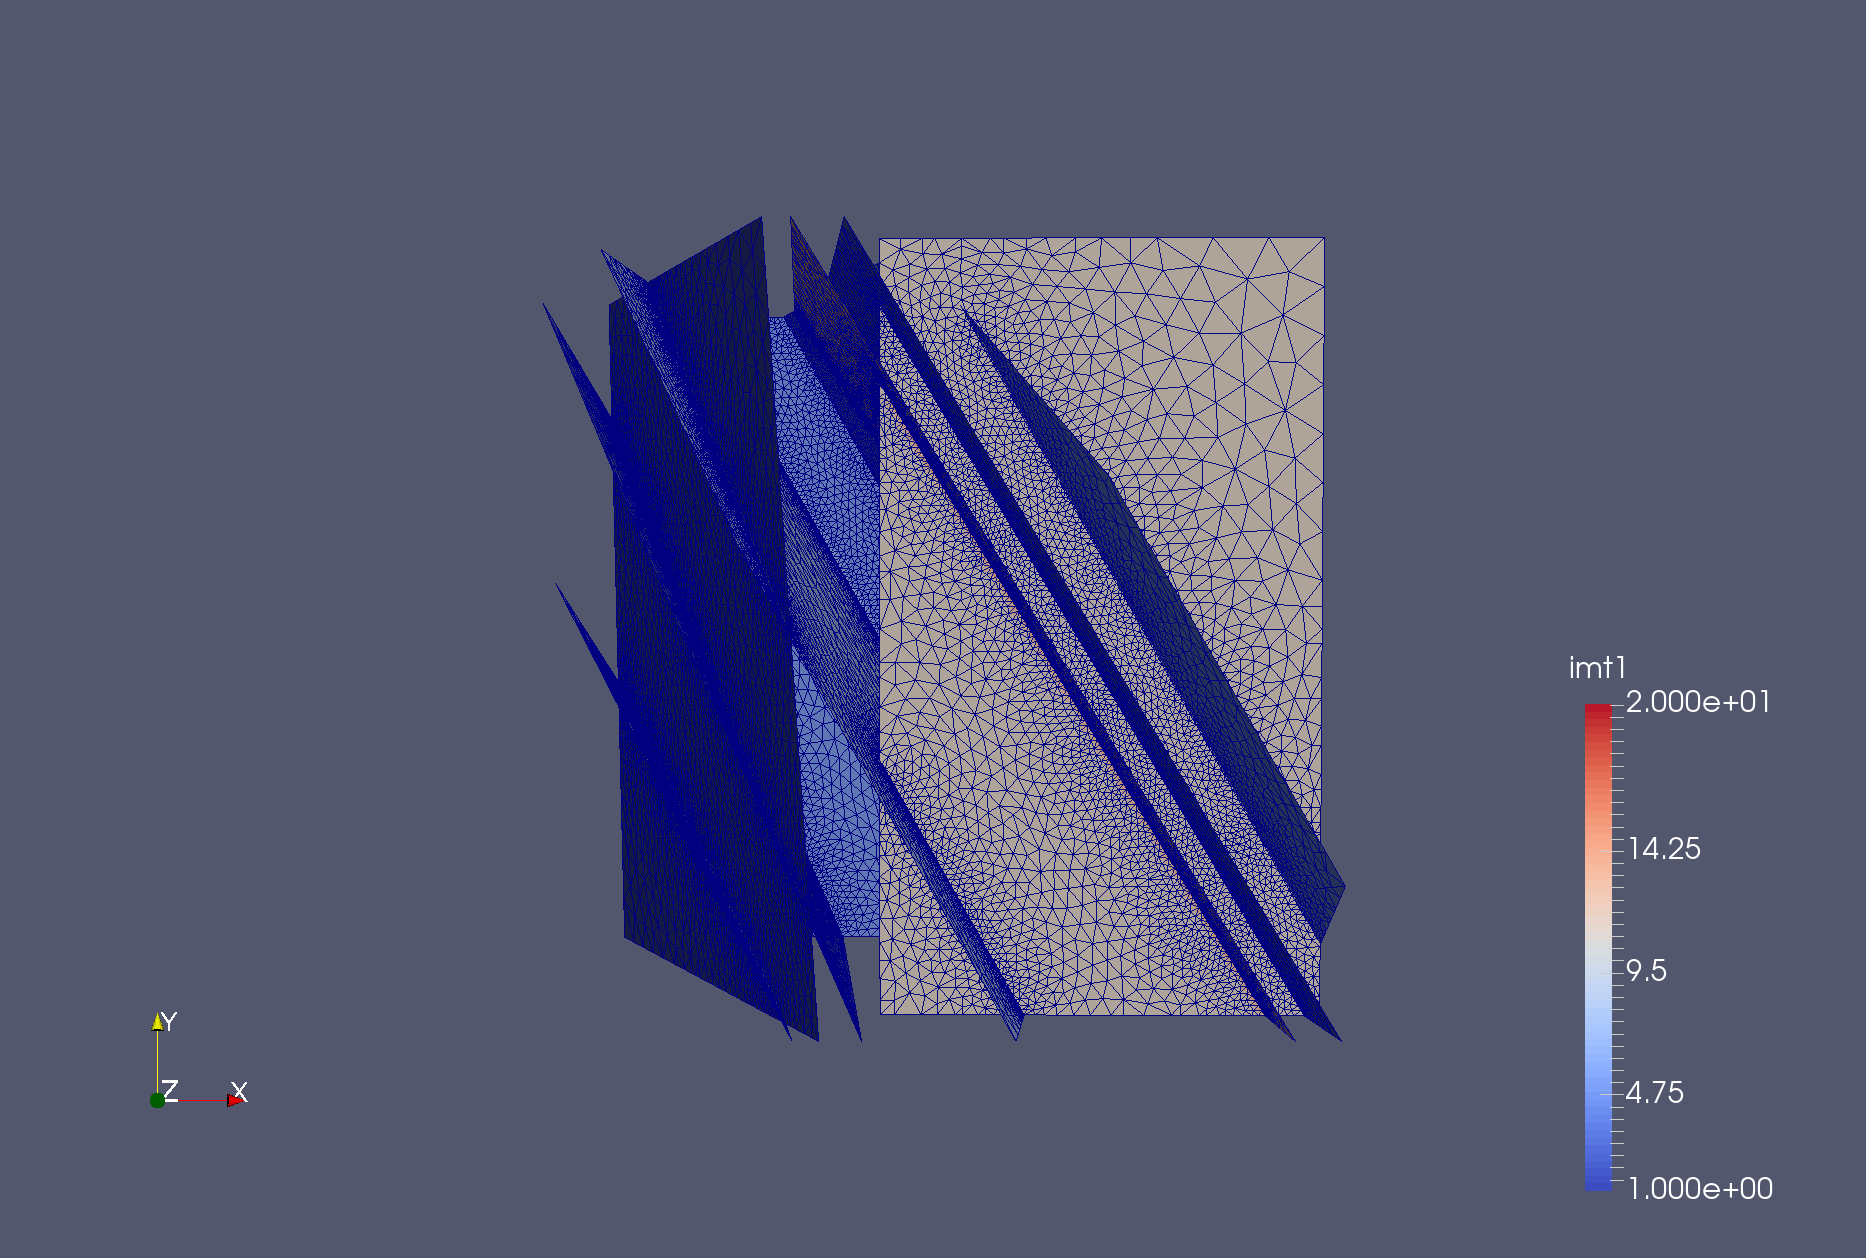
\includegraphics{lognormal_mesh.png}}\hfill}

\begin{DUlineblock}{0em}
\item[] 
\item[] 
\end{DUlineblock}

{\hfill\scalebox{1.000000}{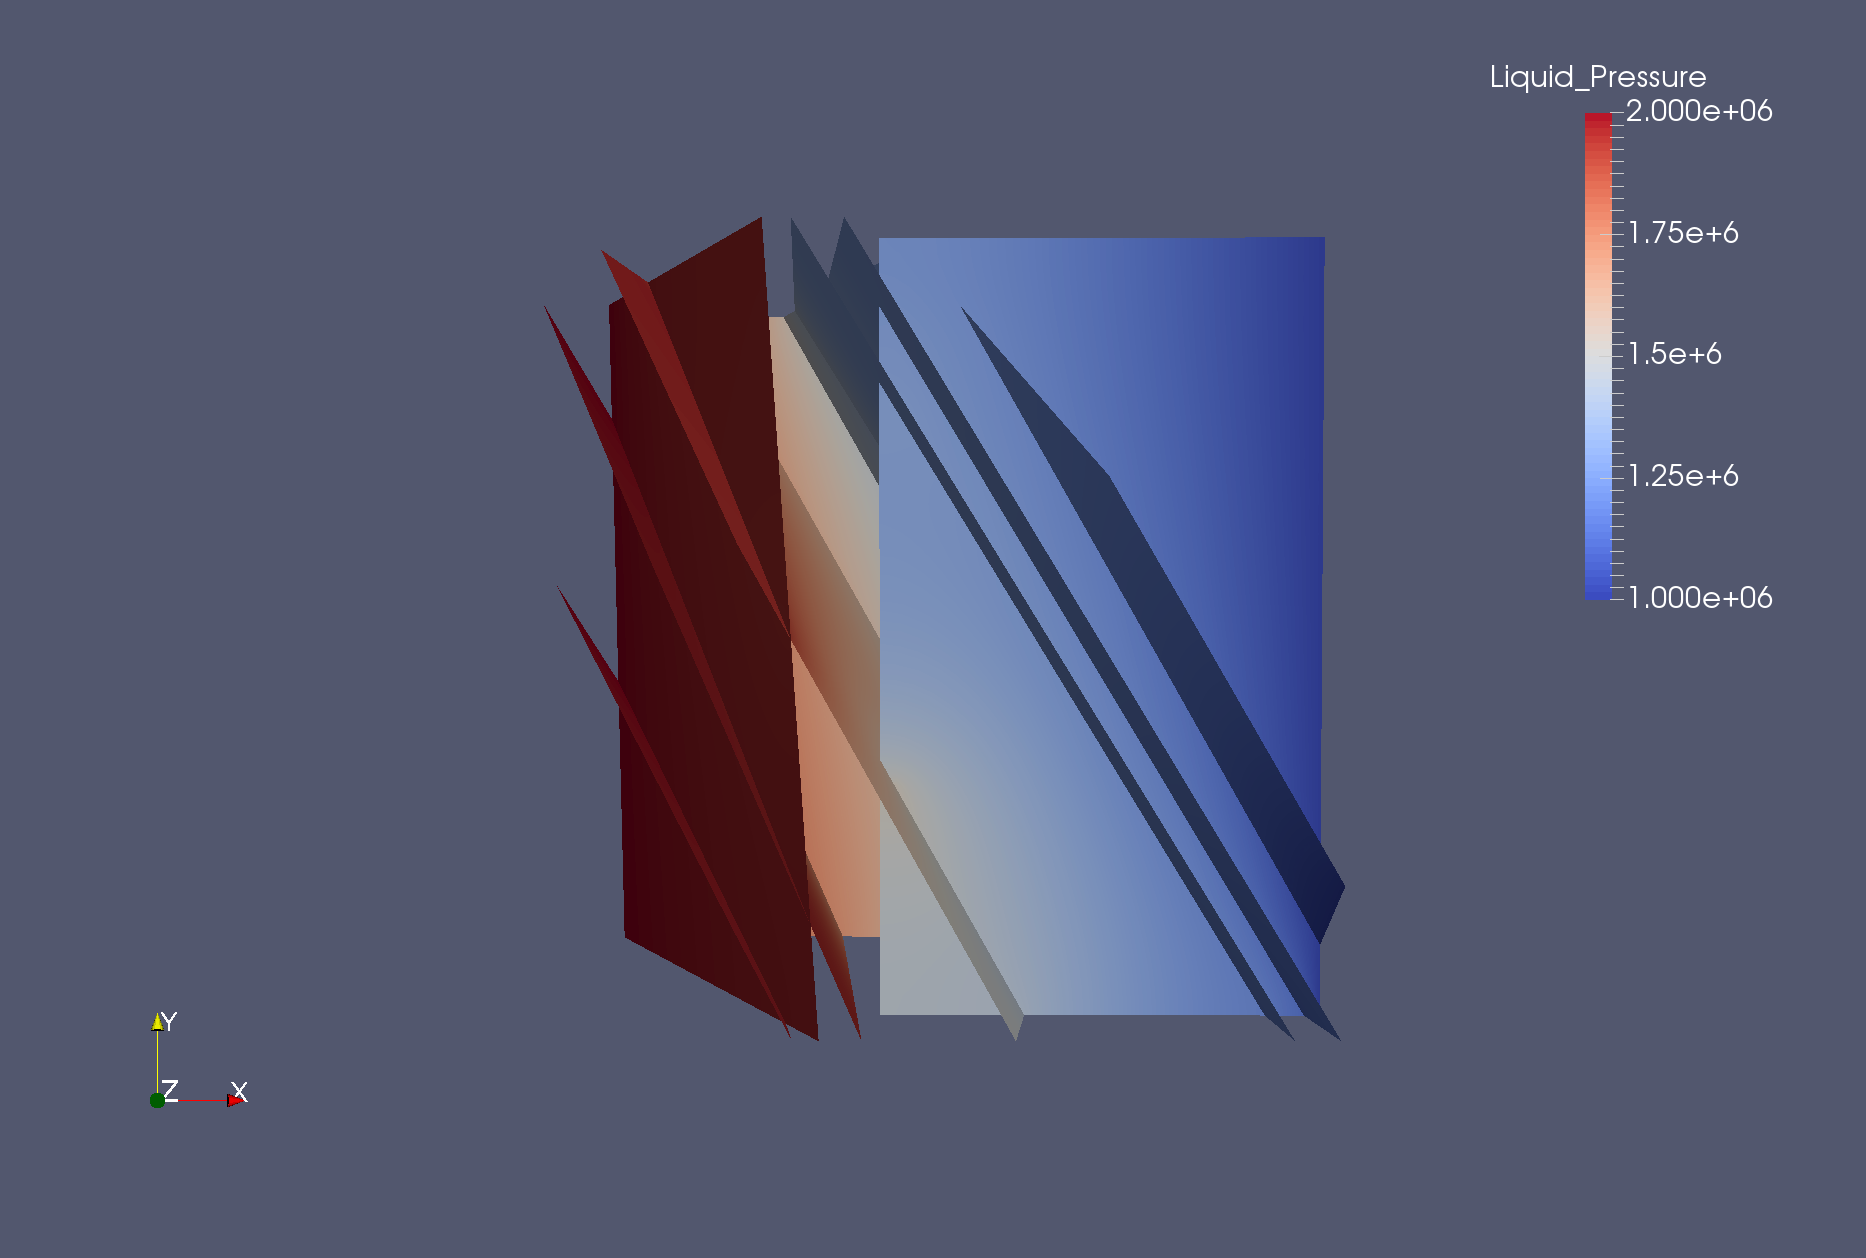
\includegraphics{lognormal_pressure.png}}\hfill}

\begin{DUlineblock}{0em}
\item[] 
\item[] 
\end{DUlineblock}

{\hfill\scalebox{1.000000}{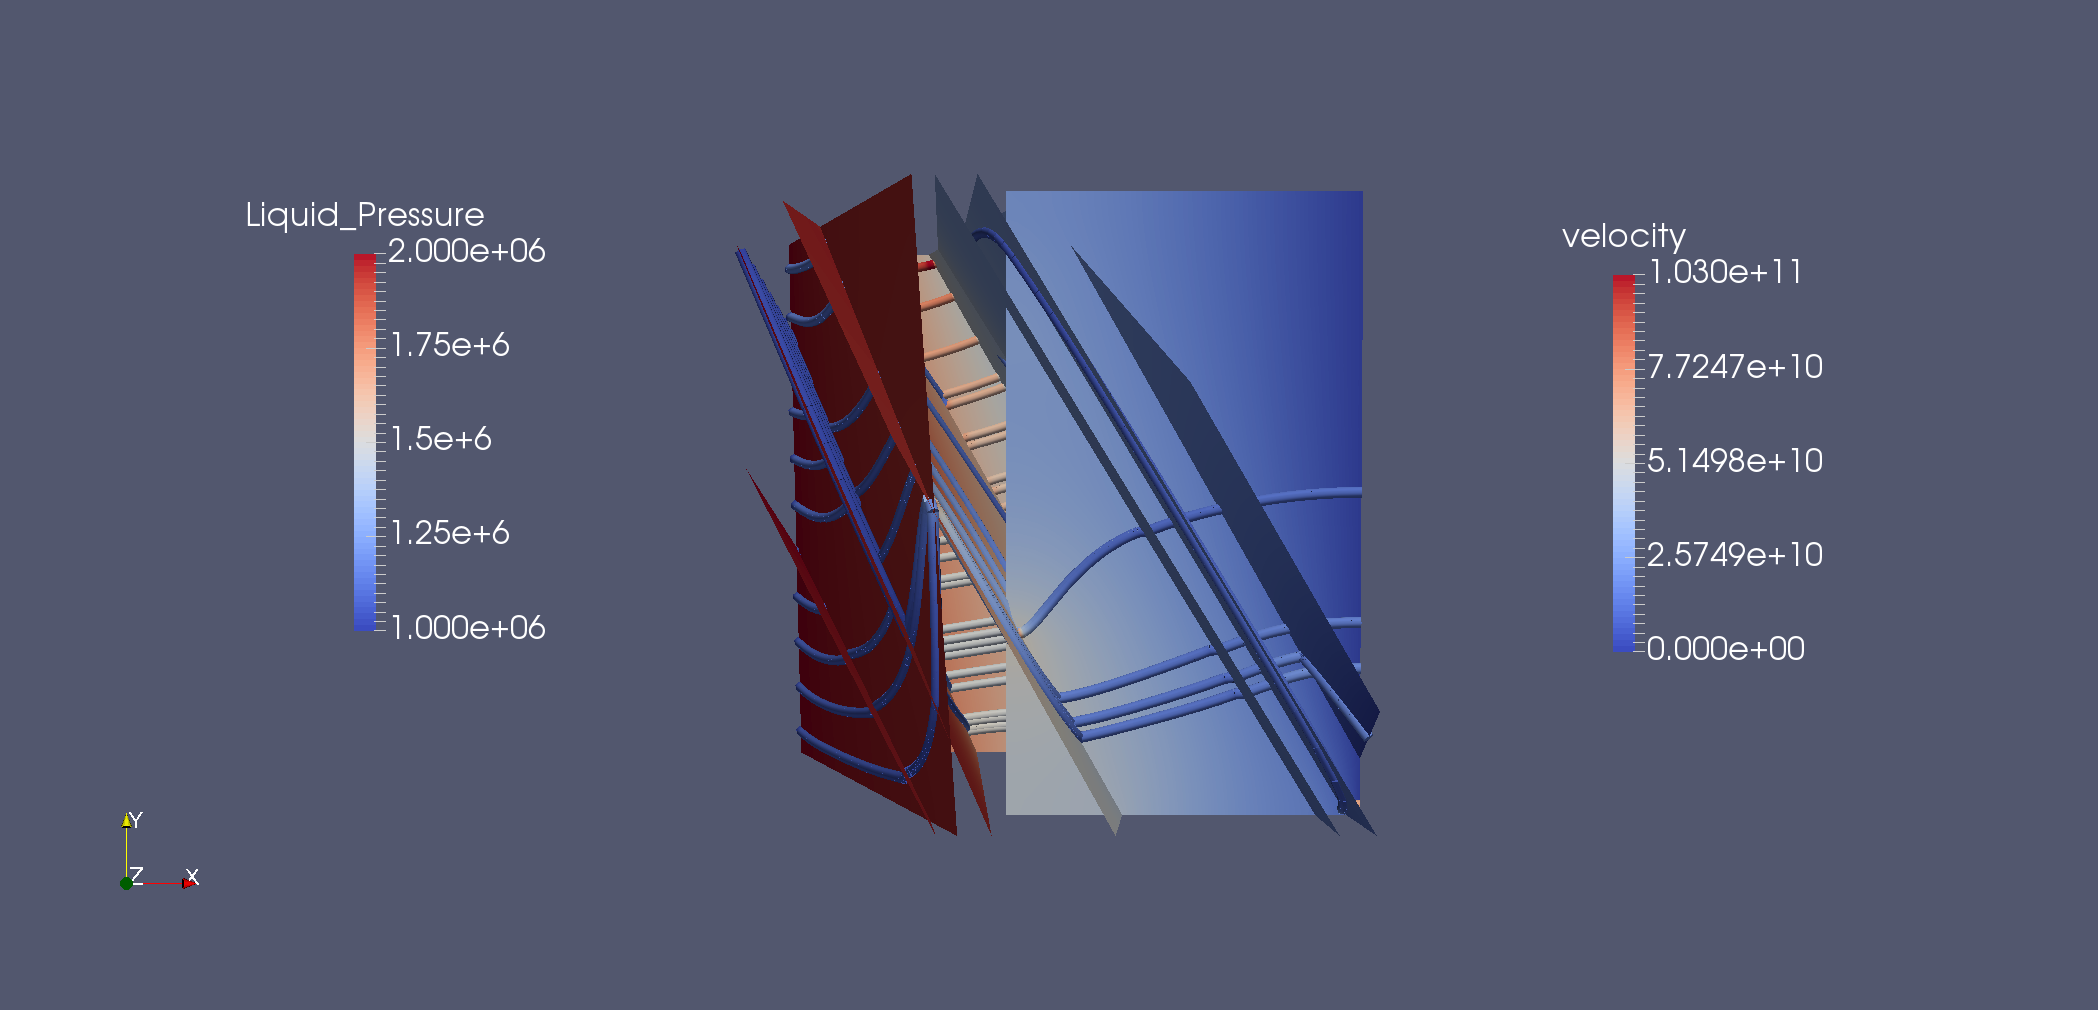
\includegraphics{lognormal_trace.png}}\hfill}

\begin{DUlineblock}{0em}
\item[] 
\item[] 
\end{DUlineblock}


\chapter{Example Applications}
\label{applications:applications-chapter}\label{applications::doc}\label{applications:example-applications}

\section{Carbon dioxide sequestration}
\label{applications:carbon-dioxide-sequestration}
DFNWORKS provides the framework necessary to perform multiphase simulations (such as flow and reactive transport) at the reservoir scale. A particular application, highlighted here, is sequestering CO2 from anthropogenic sources and disposing it in geological formations such as deep saline aquifers and abandoned oil fields. Geological CO2 sequestration is one of the principal methods under consideration to reduce carbon footprint in the atmosphere due to fossil fuels (Bachu, 2002; Pacala and Socolow, 2004). For safe and sustainable long-term storage of CO2 and to prevent leaks through existing faults and fractured rock (along with the ones created during the injection process), understanding the complex physical and chemical interactions between CO2, water (or brine) and fractured rock, is vital. DFNWORKS capability to study multiphase flow in a DFN can be used to study potential CO2 migration through cap-rock, a potential risk associated with proposed subsurface storage of CO2 in saline aquifers or depleted reservoirs. Moreover, using the reactive transport capabilities of PFLOTRAN coupled with cell-based transmissivity of the DFN allows one to study dynamically changing permeability fields with mineral precipitation and dissolution due to CO2–water interaction with rock.


\section{Shale energy extraction}
\label{applications:shale-energy-extraction}
Hydraulic fracturing (fracking) has provided access to hydrocarbon trapped in low-permeability media, such as tight shales. The process involves injecting water at high pressures to reactivate existing fractures and also create new fractures to increase permeability of the shale allowing hydrocarbons to be extracted. However, the fundamental physics of why fracking works and its long term ramifications are not well understood. Karra et al. (2015) used DFNWORKS to generate a typical production site and simulate production. Using this physics based model, they found good agreement with production field data and determined what physical mechanisms control the decline in the production curve.


\section{Nuclear waste repository}
\label{applications:nuclear-waste-repository}
The Swedish Nuclear Fuel and Waste Management Company (SKB) has undertaken a detailed investigation of the fractured granite at the Forsmark, Sweden site as a potential host formation for a subsurface repository for spent nuclear fuel (SKB, 2011; Hartley and Joyce, 2013). The Forsmark area is about 120 km north of Stockholm in northern Uppland, and the repository is proposed
to be constructed in crystalline bedrock at a depth of approximately 500 m. Based on the SKB site investigation, a statistical fracture model with multiple fracture sets was developed; detailed parameters of the Forsmark site model are in SKB (2011). We adopt a subset of the model that consist of three sets of background (non-deterministic) circular fractures whose orientations follow a Fisher distribution, fracture radii are sampled from a truncated power-law distribution, the transmissivity of the fractures is estimated using a power-law model based on the fracture radius, and the fracture aperture is related to the fracture size using the cubic law (Adler et al., 2012). Under such a formulation, the fracture apertures are uniform on each fracture, but vary among fractures. The network is generated in a cubic domain with sides of length one-kilometer. Dirichlet boundary conditions are imposed on the top (1 MPa) and bottom (2 MPa) of the domain to create a pressure gradient aligned with the vertical axis, and noflow boundary conditions are enforced along lateral boundaries.

Sources:
\begin{itemize}
\item {} 
Adler, P.M., Thovert, J.-F., Mourzenko, V.V., 2012. Fractured Porous Media. Oxford University Press, Oxford, United Kingdom.

\item {} 
Bachu, S., 2002. Sequestration of CO2 in geological media in response to climate change: road map for site selection using the transform of the geological space into the CO2 phase space. Energy Convers. Manag. 43, 87–102.

\item {} 
Hartley, L., Joyce, S., 2013. Approaches and algorithms for groundwater flow modeling in support of site investigations and safety assessment of the Fors- mark site, Sweden. J. Hydrol. 500, 200–216.

\item {} 
Karra, S., Makedonska, N., Viswanathan, H., Painter, S., Hyman, J., 2015. Effect of advective flow in fractures and matrix diffusion on natural gas production. Water Resour. Res., under review.

\item {} 
Pacala, S., Socolow, R., 2004. Stabilization wedges: solving the climate problem for the next 50 years with current technologies. Science 305, 968–972.

\item {} 
SKB, Long-Term Safety for the Final Repository for Spent Nuclear Fuel at Forsmark. Main Report of the SR-Site Project. Technical Report SKB TR-11-01, Swedish Nuclear Fuel and Waste Management Co., Stockholm, Sweden, 2011.

\end{itemize}


\renewcommand{\indexname}{Python Module Index}
\begin{theindex}
\def\bigletter#1{{\Large\sffamily#1}\nopagebreak\vspace{1mm}}
\bigletter{l}
\item {\texttt{lagrit\_scripts.py}}, \pageref{pydfnworks:module-lagrit_scripts.py}
\indexspace
\bigletter{m}
\item {\texttt{mesh\_dfn\_helper.py}}, \pageref{pydfnworks:module-mesh_dfn_helper.py}
\item {\texttt{meshdfn.py}}, \pageref{pydfnworks:module-meshdfn.py}
\indexspace
\bigletter{p}
\item {\texttt{pydfnworks.distributions}}, \pageref{pydfnworks:module-pydfnworks.distributions}
\item {\texttt{pydfnworks.flow}}, \pageref{pydfnworks:module-pydfnworks.flow}
\item {\texttt{pydfnworks.gen\_input}}, \pageref{pydfnworks:module-pydfnworks.gen_input}
\item {\texttt{pydfnworks.gen\_output}}, \pageref{pydfnworks:module-pydfnworks.gen_output}
\item {\texttt{pydfnworks.generator}}, \pageref{pydfnworks:module-pydfnworks.generator}
\item {\texttt{pydfnworks.helper}}, \pageref{pydfnworks:module-pydfnworks.helper}
\item {\texttt{pydfnworks.lagrit\_scripts}}, \pageref{pydfnworks:module-pydfnworks.lagrit_scripts}
\item {\texttt{pydfnworks.legal}}, \pageref{pydfnworks:module-pydfnworks.legal}
\item {\texttt{pydfnworks.mesh\_dfn\_helper}}, \pageref{pydfnworks:module-pydfnworks.mesh_dfn_helper}
\item {\texttt{pydfnworks.meshdfn}}, \pageref{pydfnworks:module-pydfnworks.meshdfn}
\item {\texttt{pydfnworks.run\_meshing}}, \pageref{pydfnworks:module-pydfnworks.run_meshing}
\item {\texttt{pydfnworks.transport}}, \pageref{pydfnworks:module-pydfnworks.transport}
\indexspace
\bigletter{r}
\item {\texttt{run\_meshing.py}}, \pageref{pydfnworks:module-run_meshing.py}
\end{theindex}

\renewcommand{\indexname}{Index}
\printindex
\end{document}
